\documentclass{beamer}
\usepackage[english]{babel}
\usepackage{amsmath,amssymb,graphicx,hyperref}

%%%%%%%%%% Start TeXmacs macros
\newcommand{\mathd}{\mathrm{d}}
\newcommand{\nospace}{}
\newcommand{\tmfoldedstd}[2]{\trivlist{\item[$\bullet$]\mbox{}#1}}
%%%%%%%%%% End TeXmacs macros

\begin{document}

{\screens{\begin{frame}
  \
  
  \
  
  \
  
  \
  
  \
  
  \title{计算视觉与模式识别}
  
  \maketitle
  
  \ 
\end{frame}}{\begin{frame}
  \frametitle{灰度变换与空间域滤波}
  \begin{eqnarray*}
    g (x, y) & = & T [f]
  \end{eqnarray*}
  其中
  \begin{eqnarray*}
    g, f & : & (R, R) \mapsto R
  \end{eqnarray*}
\end{frame}}{\begin{frame}
  \frametitle{灰度变换}
  \begin{eqnarray*}
    s & = & T (r)
  \end{eqnarray*}
  其中
  \begin{eqnarray*}
    s & = & g (x, y)\\
    r & = & f (x, y)\\
    g (x, y) & = & T (f (x, y))
  \end{eqnarray*}
\end{frame}}{\begin{frame}
  \frametitle{示例1}
  
  \
  
  \
  
  \resizebox{1\columnwidth}{!}{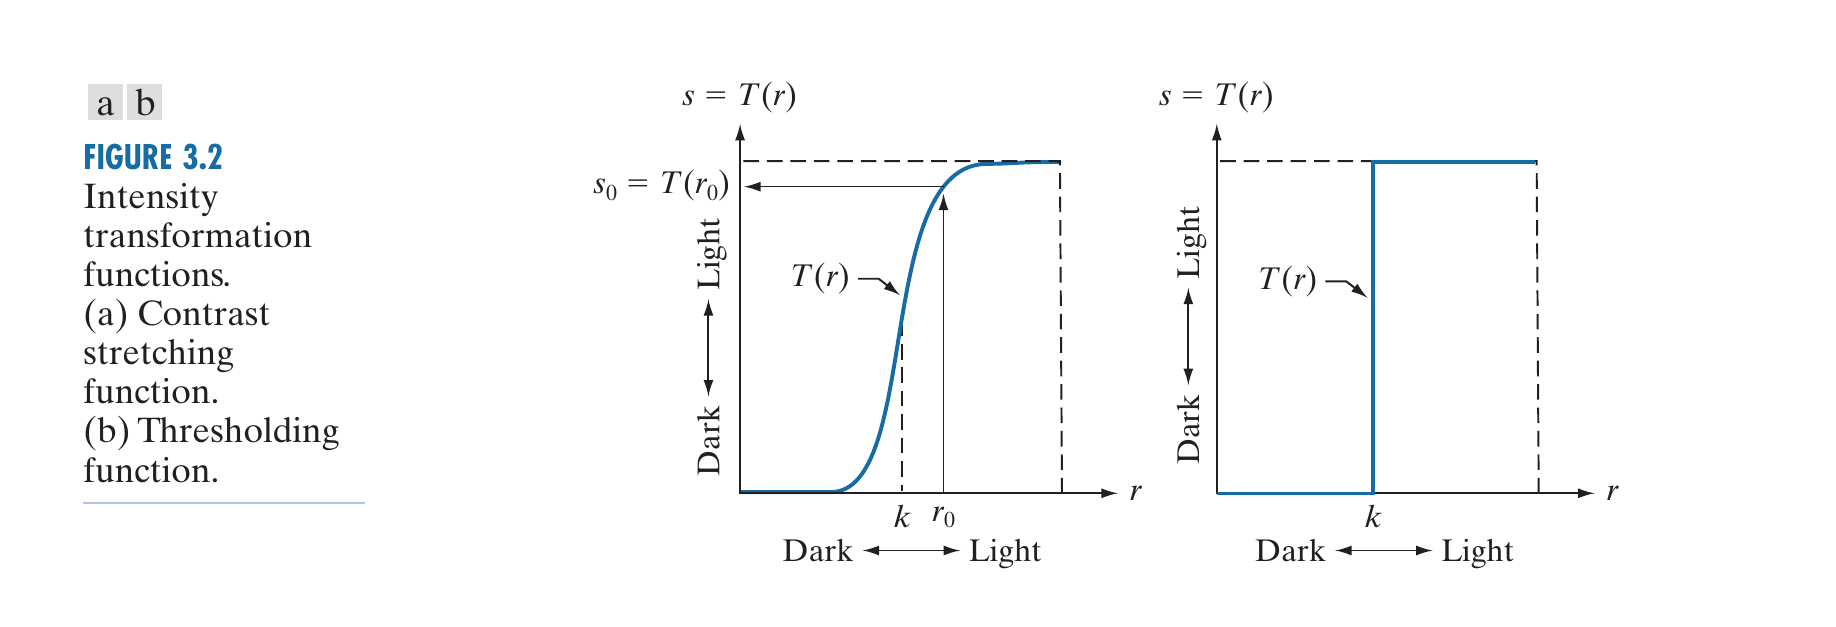
\includegraphics{img/intensity_transformation.png}}
\end{frame}}{\begin{frame}
  \frametitle{示例2}
  
  \resizebox{1\columnwidth}{!}{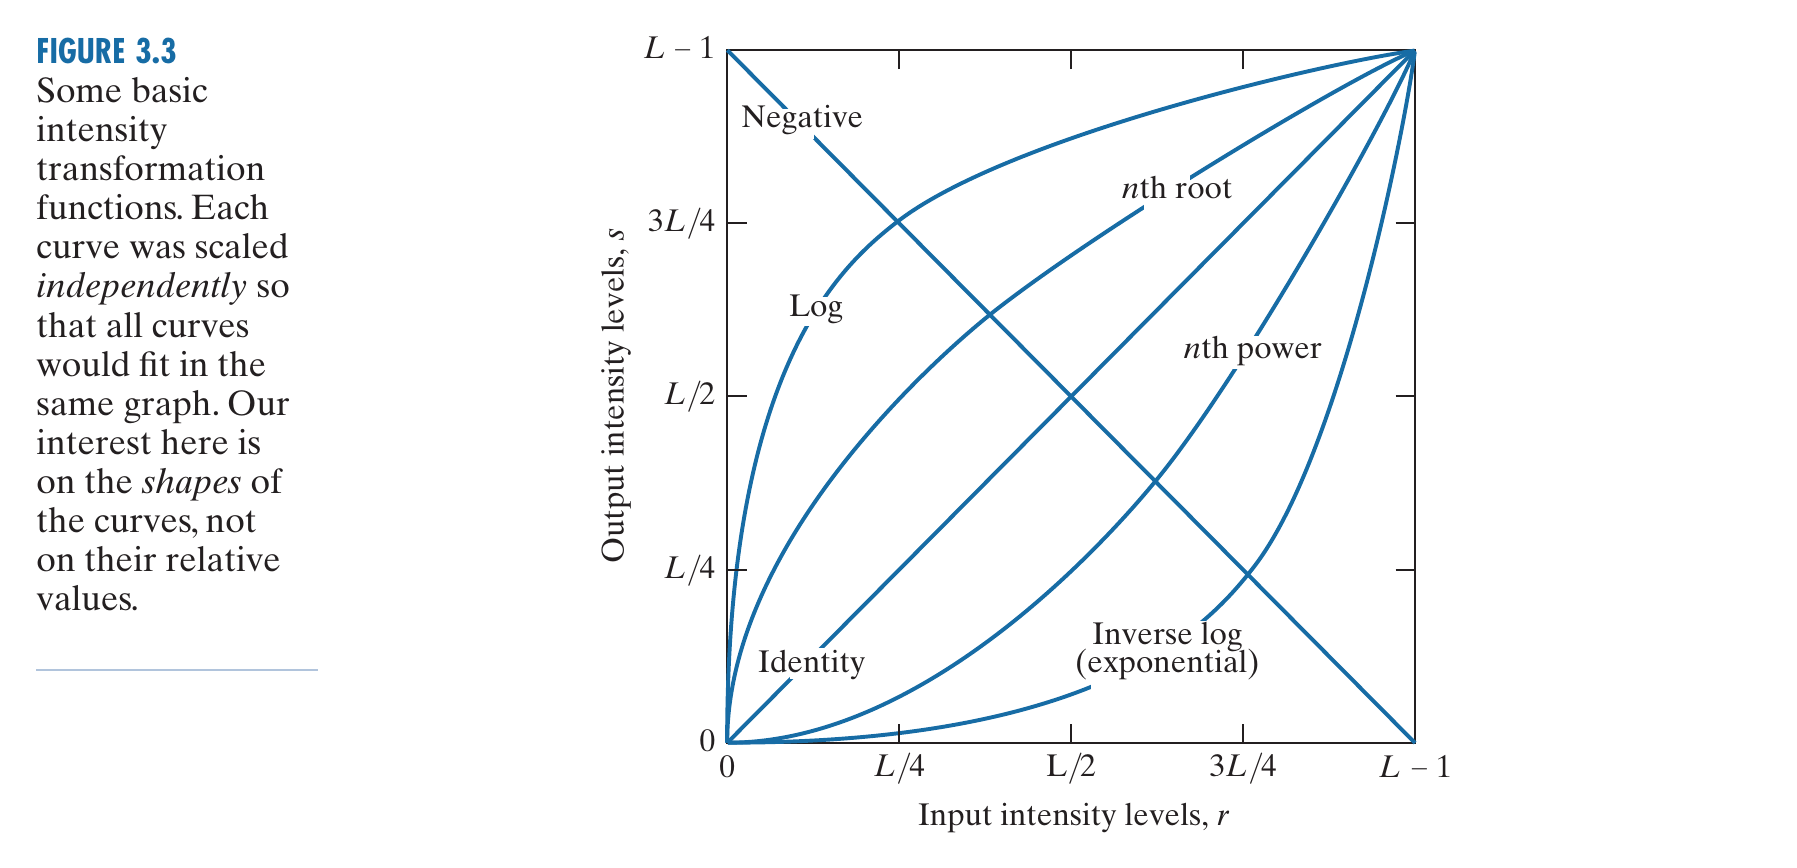
\includegraphics{img/some_basic_intensity_transformation_functions.png}}
\end{frame}}{\begin{frame}
  \frametitle{$s = L - 1 - r$}
  
  \resizebox{1\columnwidth}{!}{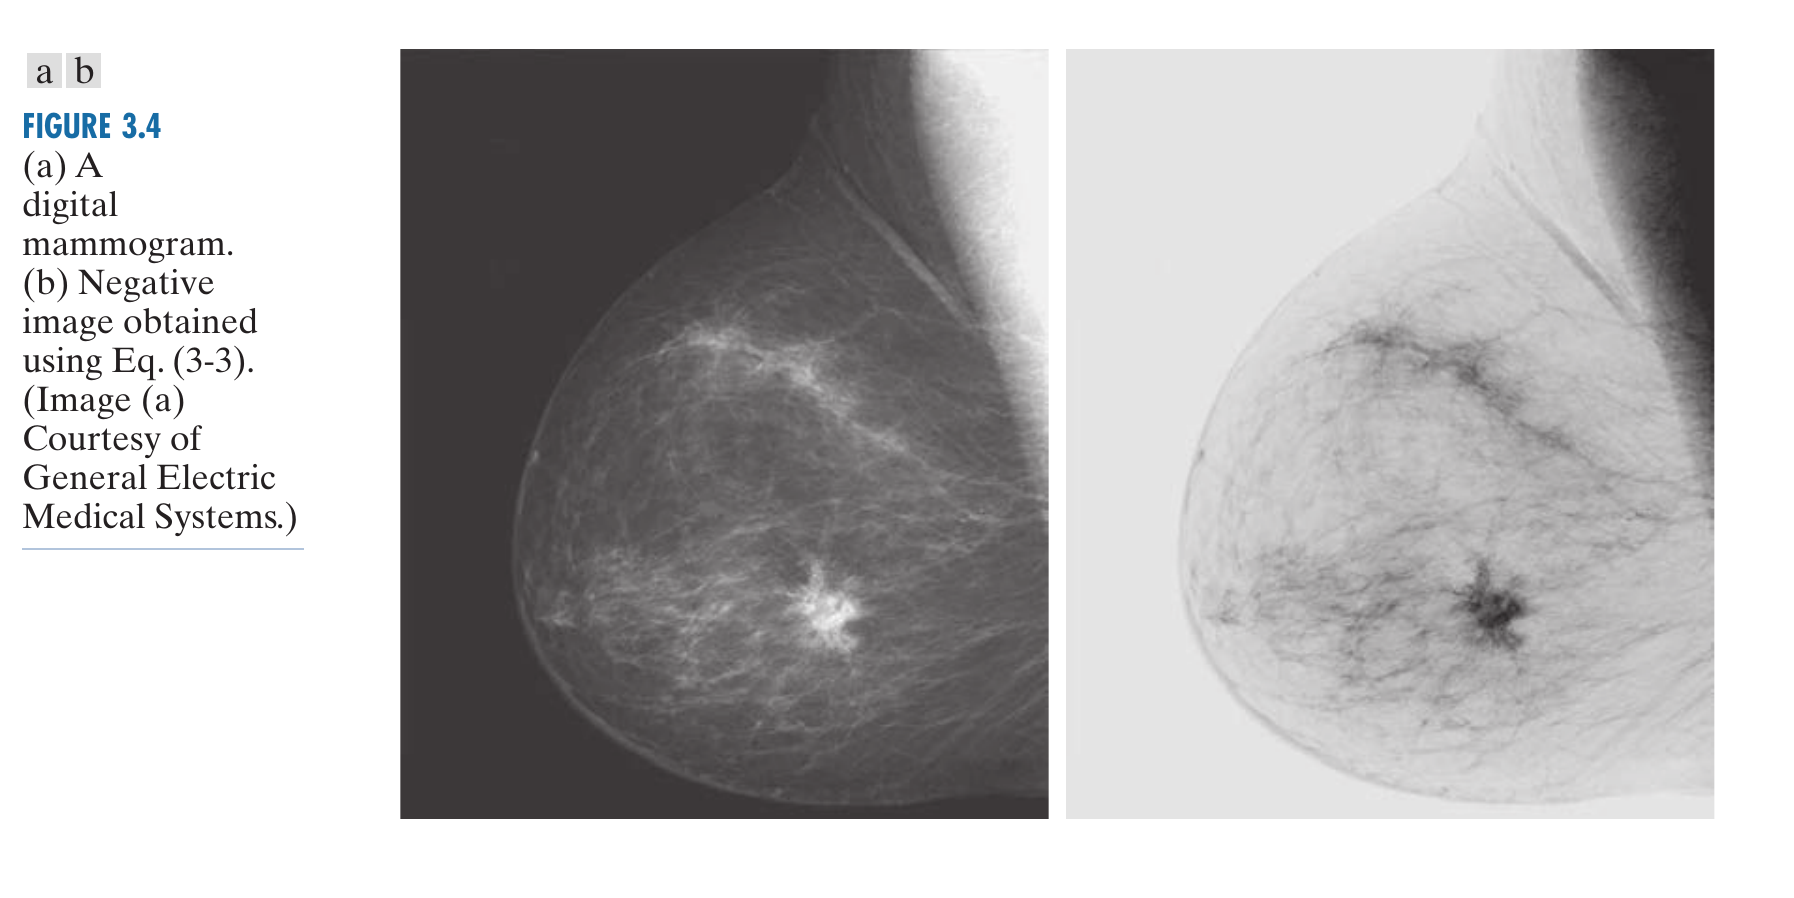
\includegraphics{img/digital_mammogram_negative.png}}
\end{frame}}{\begin{frame}
  \frametitle{$s = \ln (1 + r)$}
  
  \resizebox{1\columnwidth}{!}{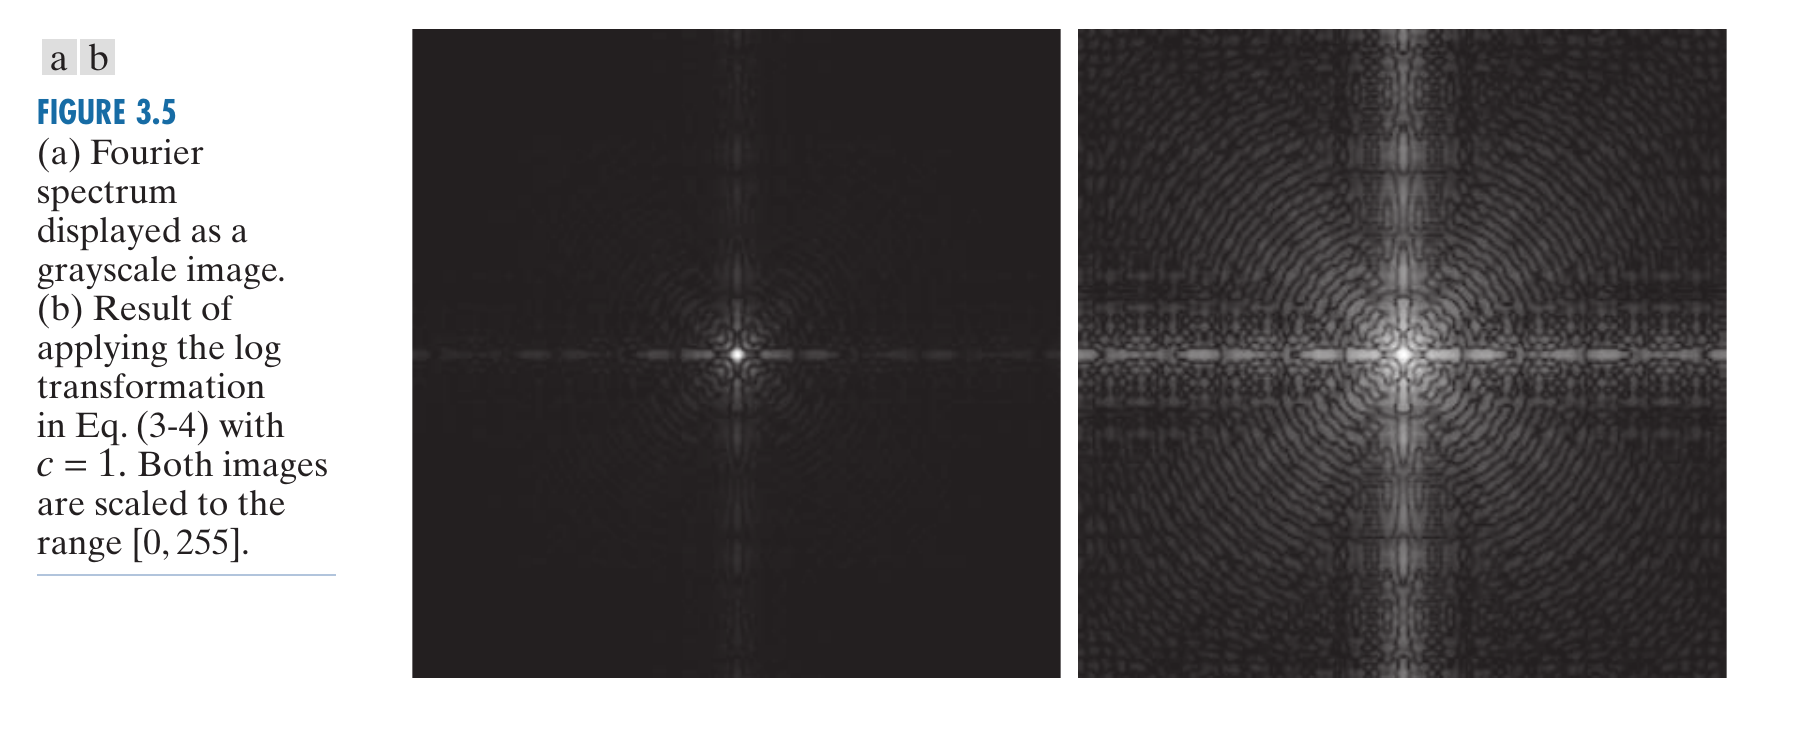
\includegraphics{img/log_fourier.png}}
\end{frame}}{\begin{frame}
  \frametitle{$s = c \nospace r^{\gamma}$}
  
  \resizebox{1\columnwidth}{!}{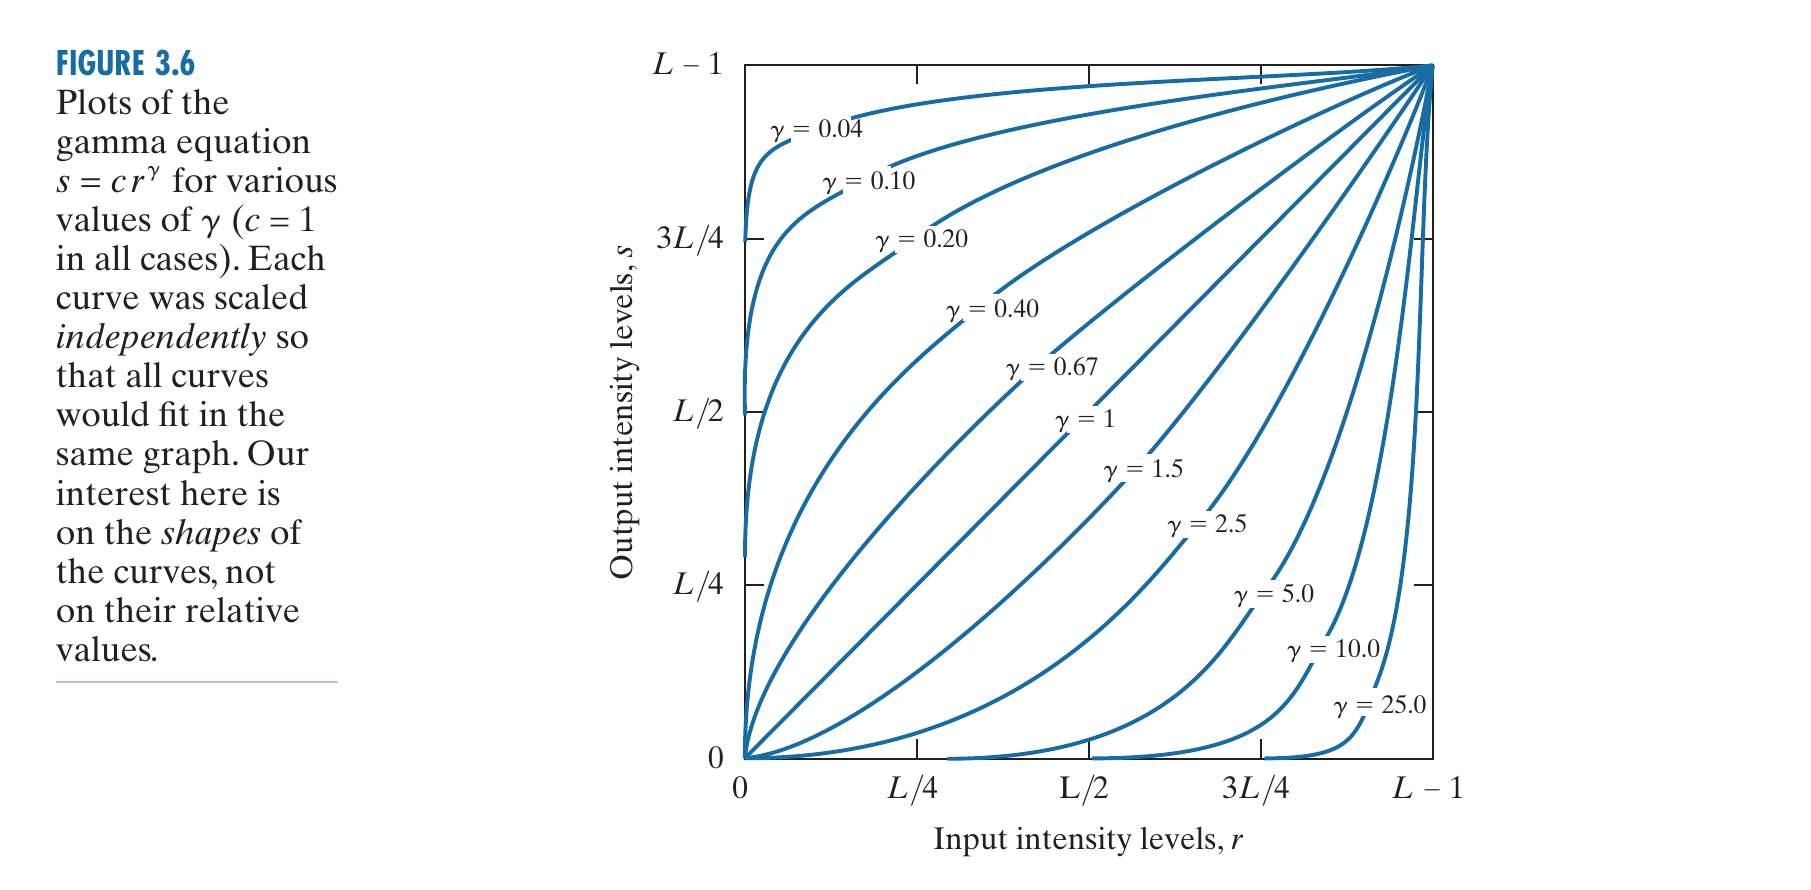
\includegraphics{img/gamma_equation.png}}
\end{frame}}{\begin{frame}
  \resizebox{1\columnwidth}{!}{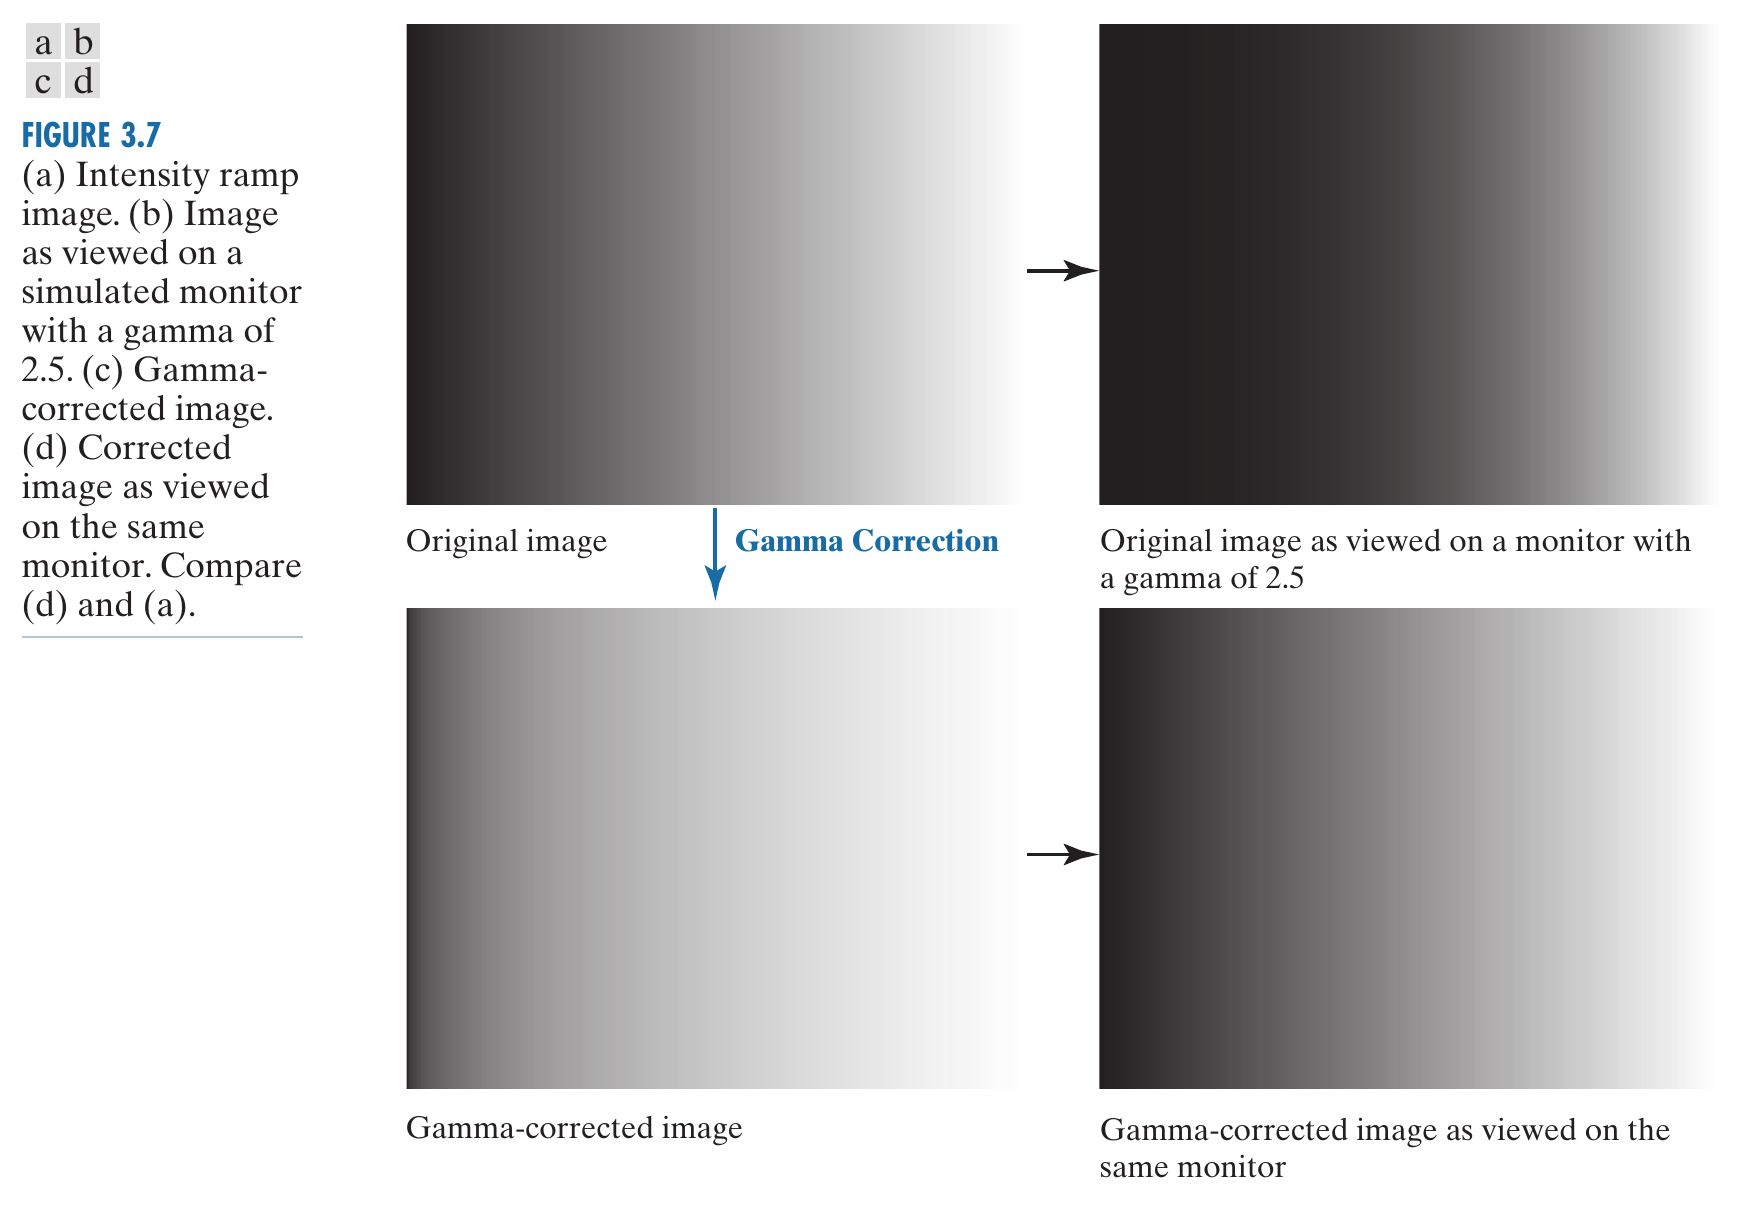
\includegraphics{img/intensity_ramp_gamma_correction.png}}
\end{frame}}{\begin{frame}
  {\hspace{3em}}\resizebox{0.8\columnwidth}{!}{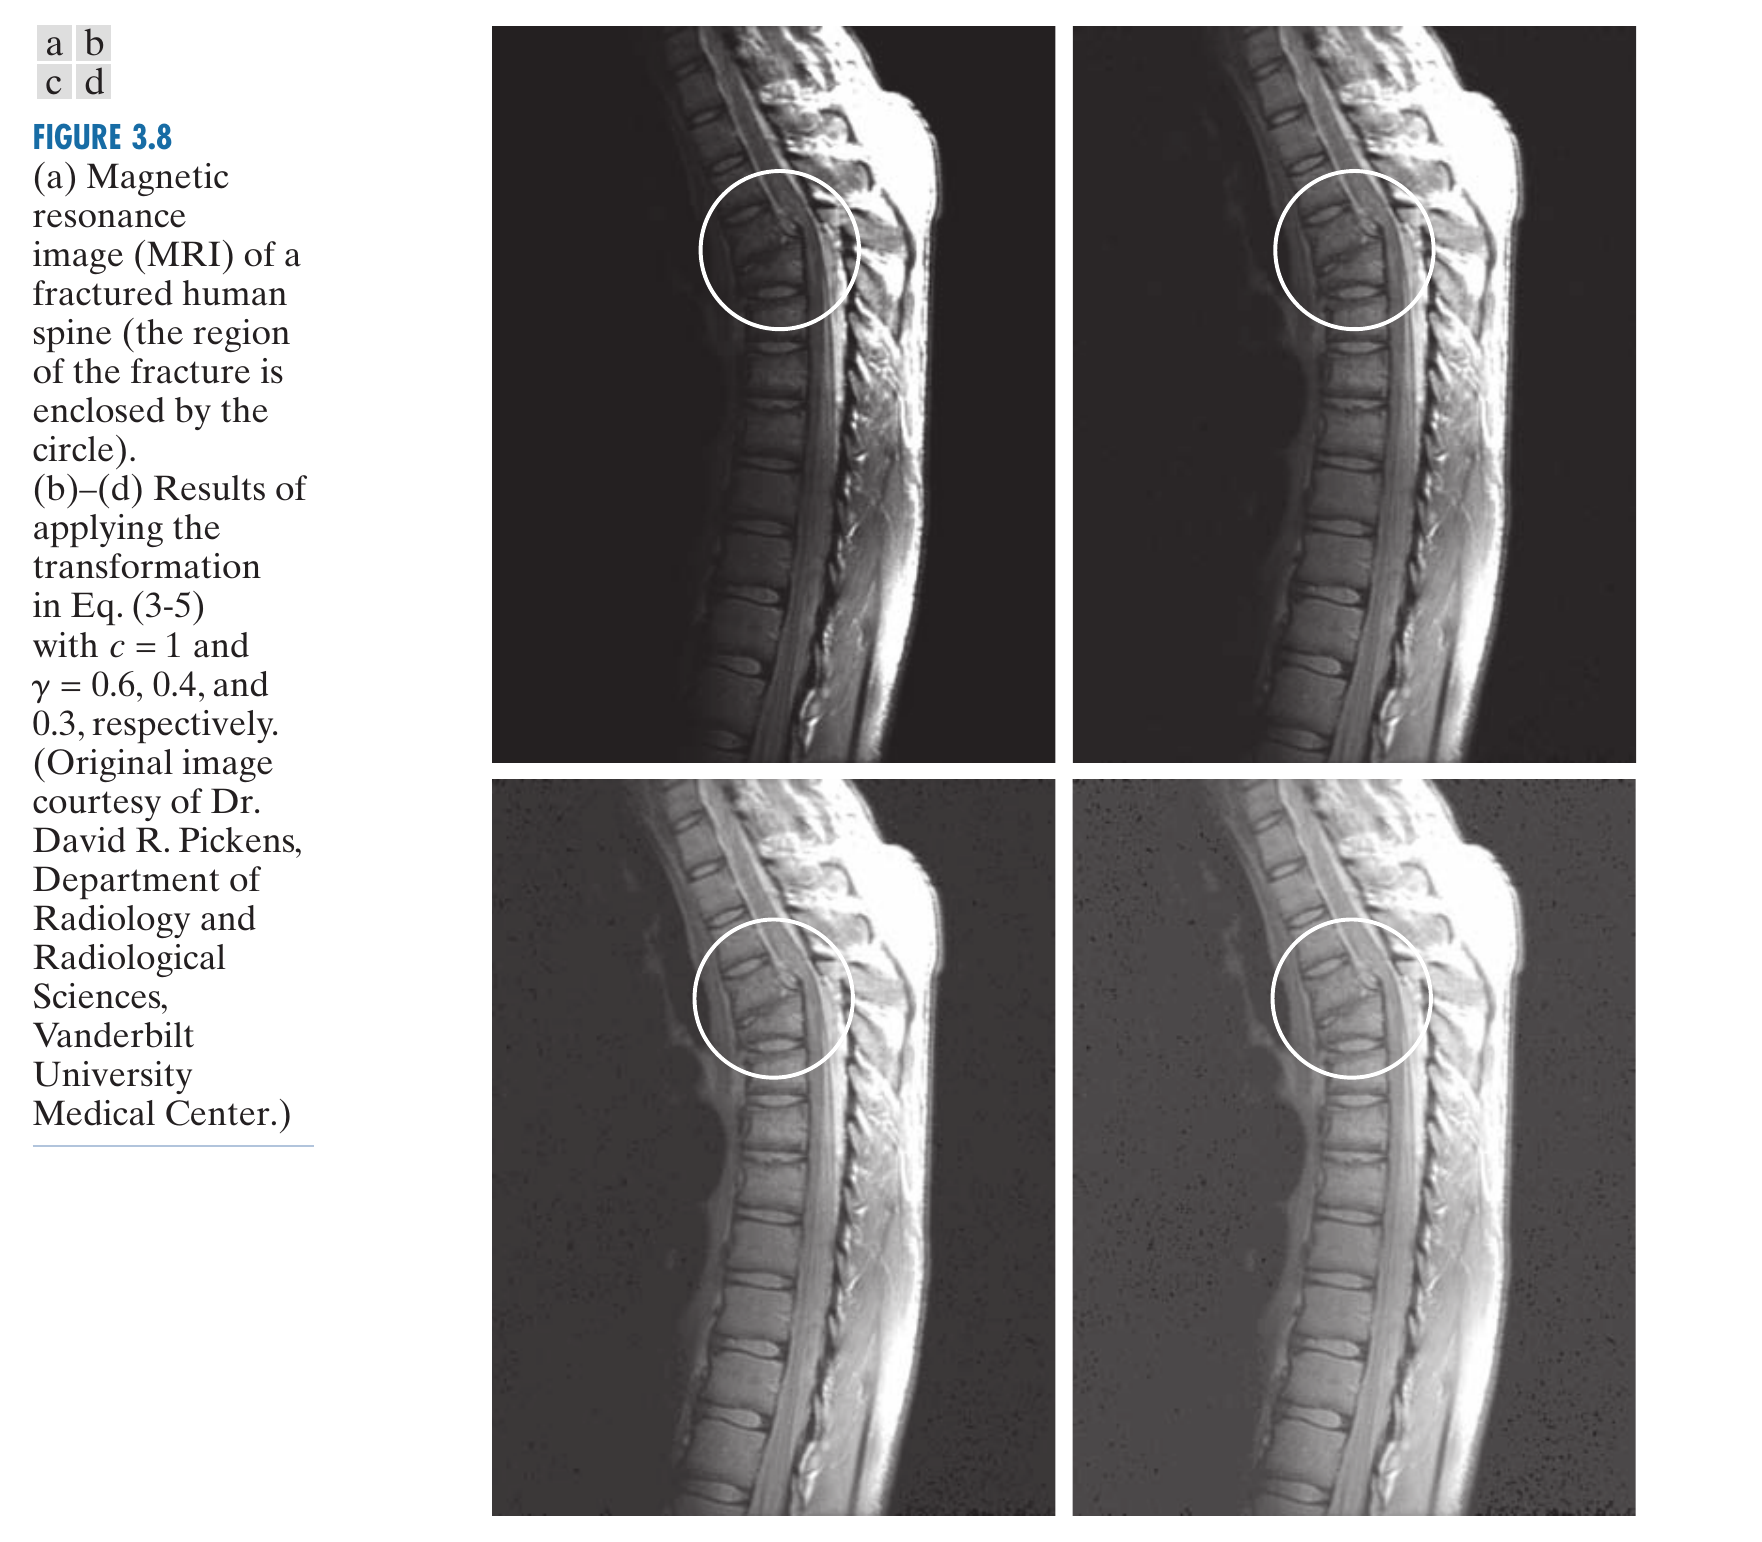
\includegraphics{img/gamma_mri.png}}
\end{frame}}{\begin{frame}
  \qquad\resizebox{0.9\columnwidth}{!}{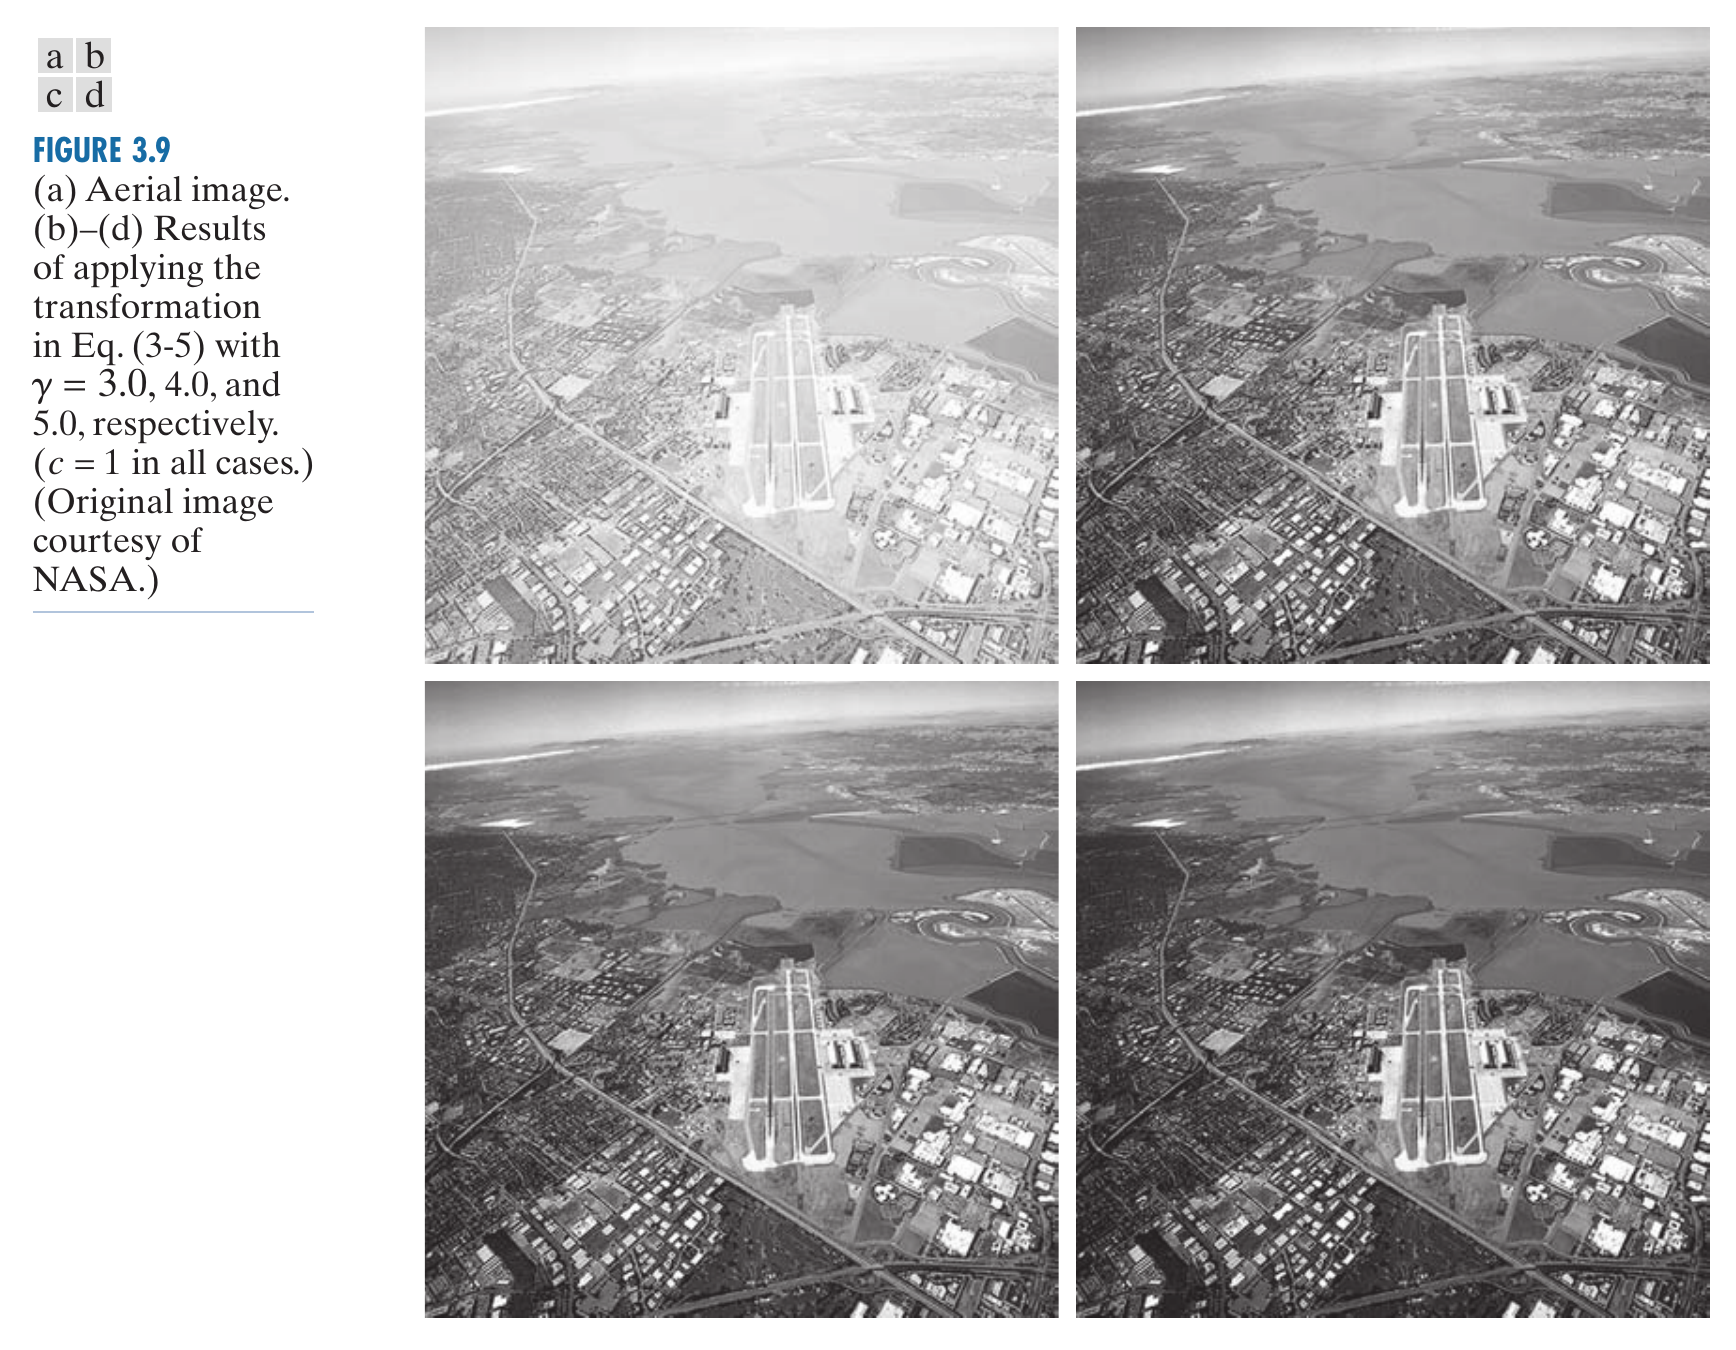
\includegraphics{img/gamma_aerial.png}}
\end{frame}}{\begin{frame}
  \quad\resizebox{0.9\columnwidth}{!}{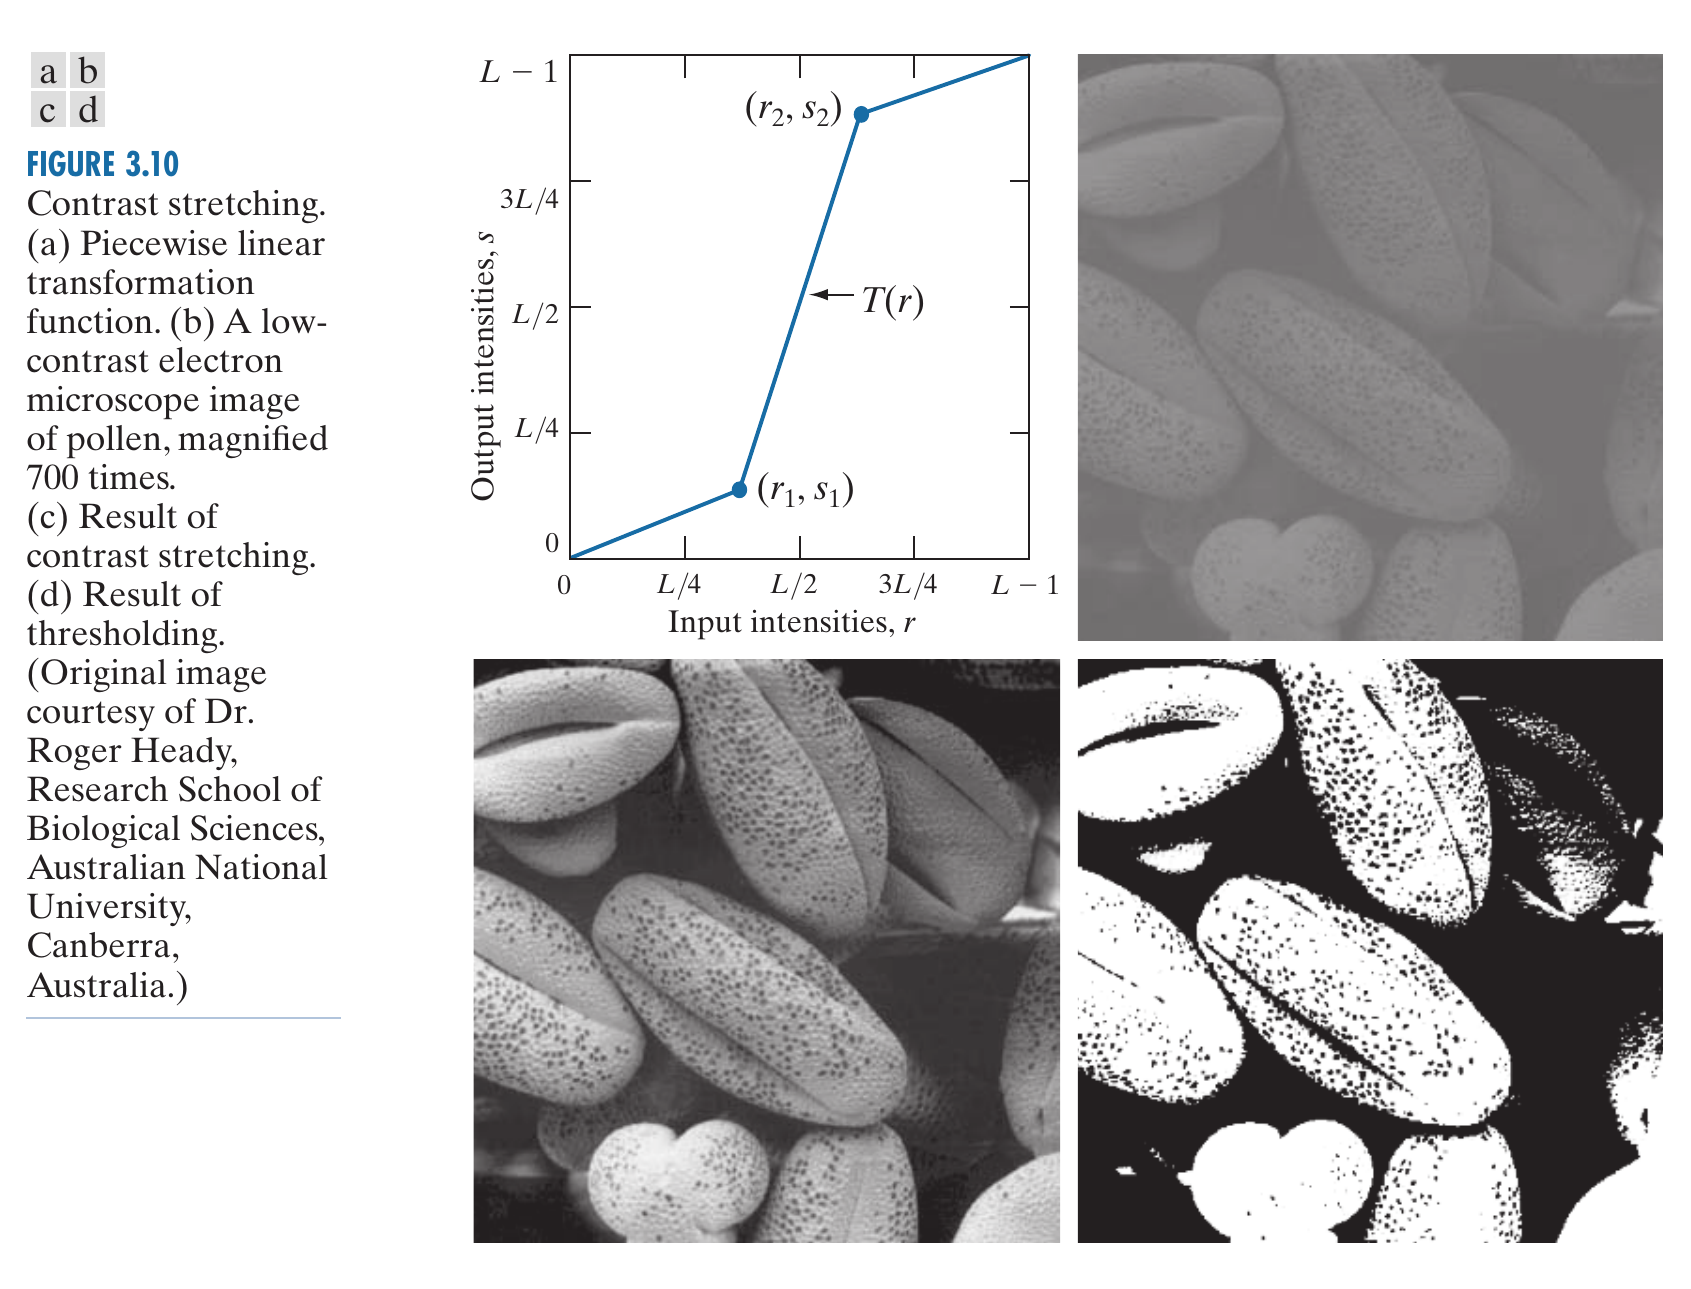
\includegraphics{img/contrast_stretching.png}}
\end{frame}}{\begin{frame}
  \frametitle{亮度分层}
  
  \
  
  \
  
  \resizebox{1\columnwidth}{!}{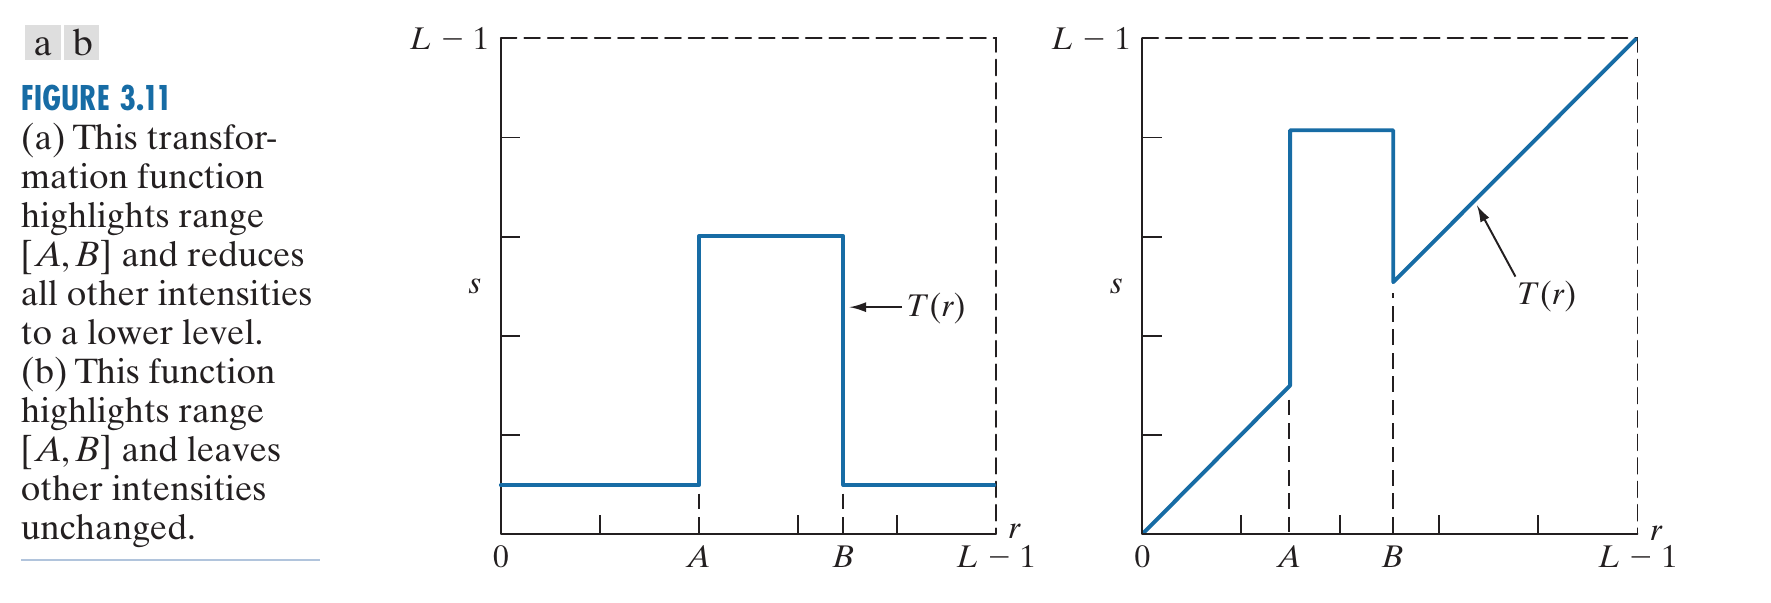
\includegraphics{img/highlights_range_a_b.png}}
  
  \ 
\end{frame}}{\begin{frame}
  \
  
  \resizebox{1\columnwidth}{!}{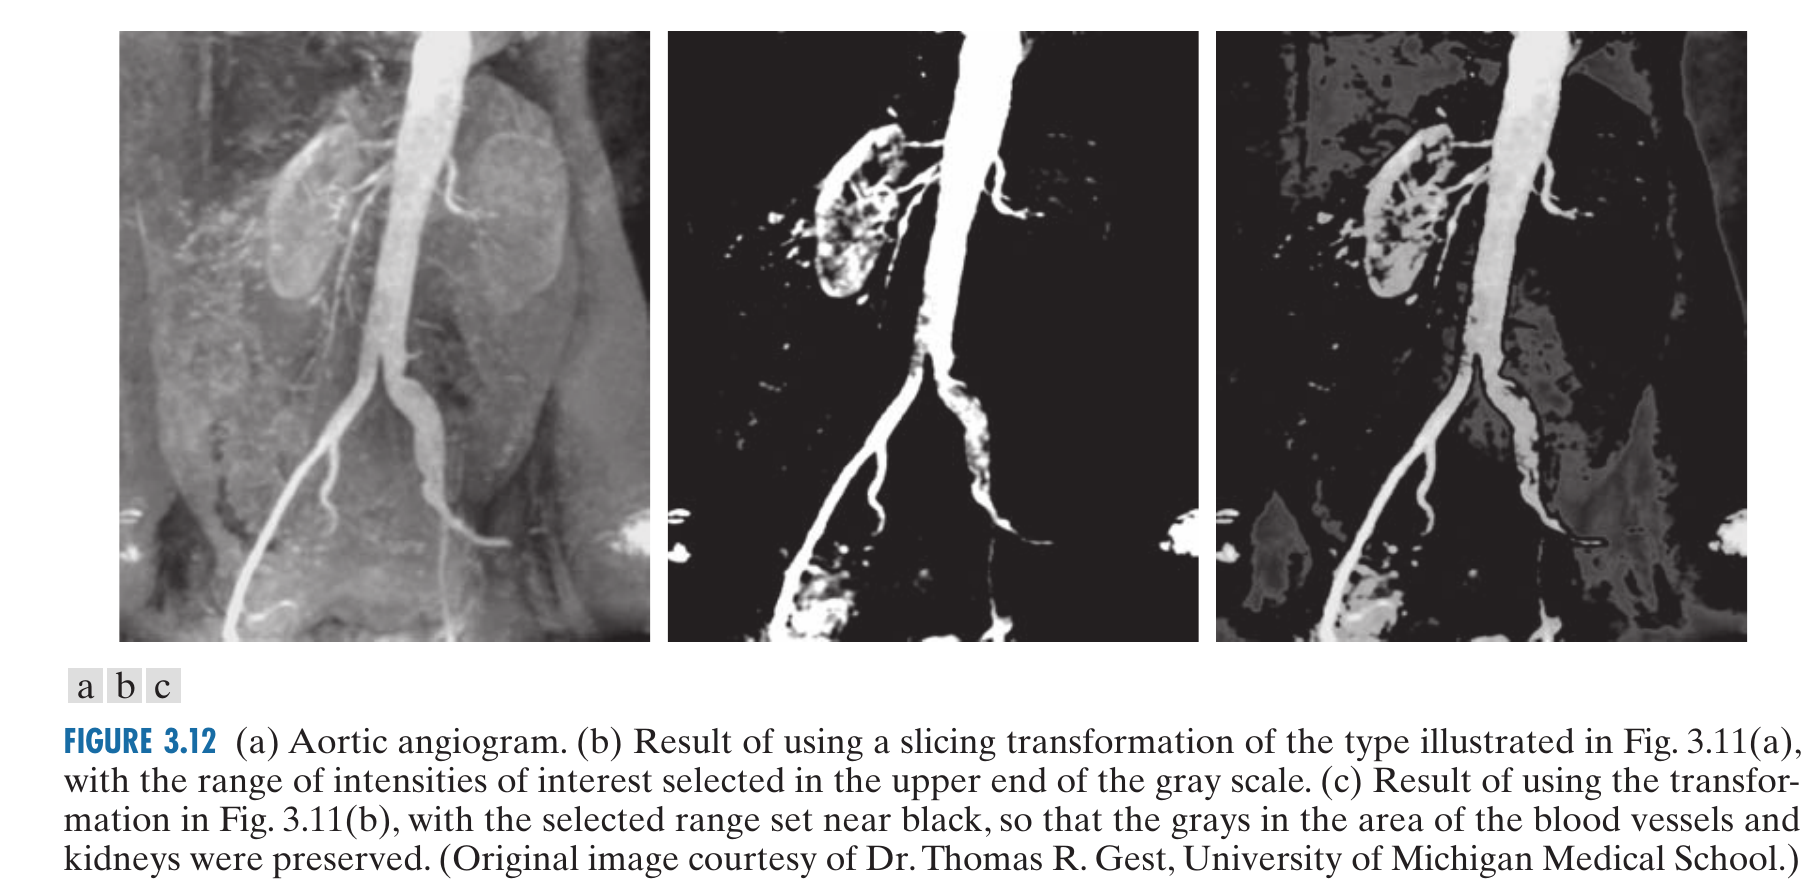
\includegraphics{img/aortic_angiogram_highlight_range.png}}
\end{frame}}{\begin{frame}
  \frametitle{位平面分层}
  
  \resizebox{1\columnwidth}{!}{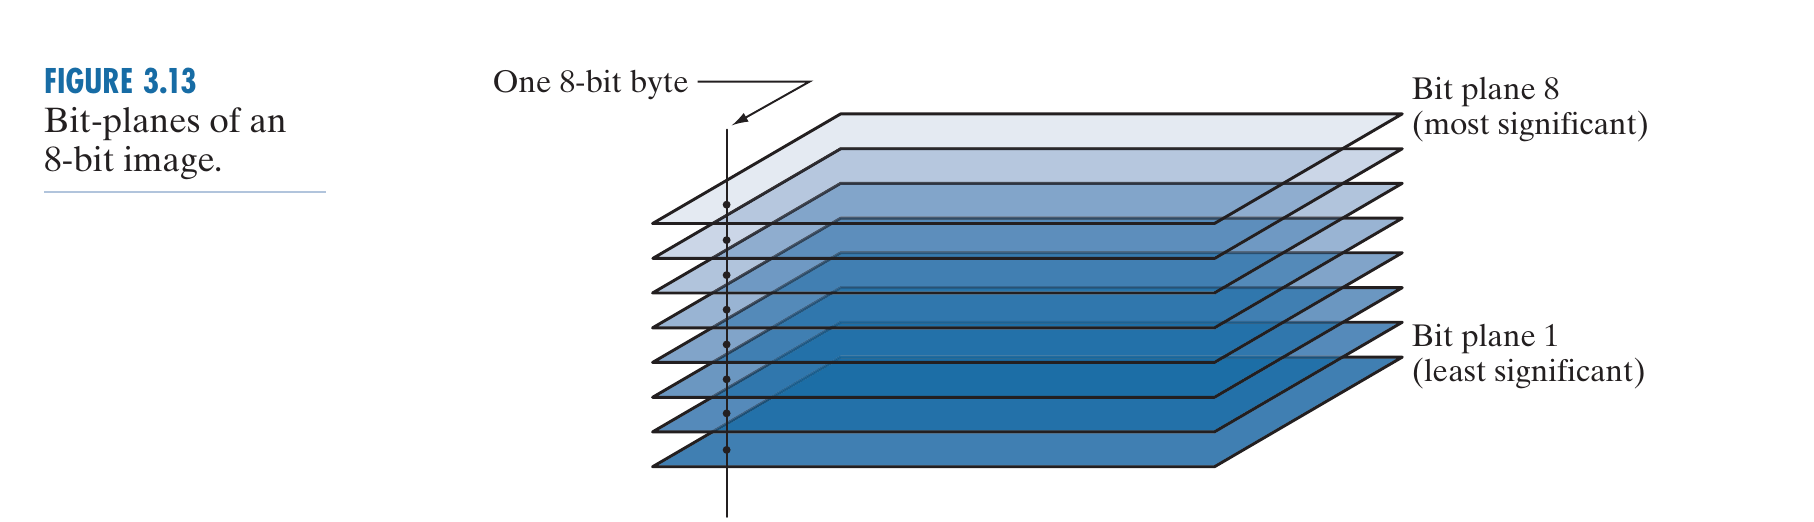
\includegraphics{img/8_bit_planes.png}}
\end{frame}}{\begin{frame}
  \
  
  \resizebox{1\columnwidth}{!}{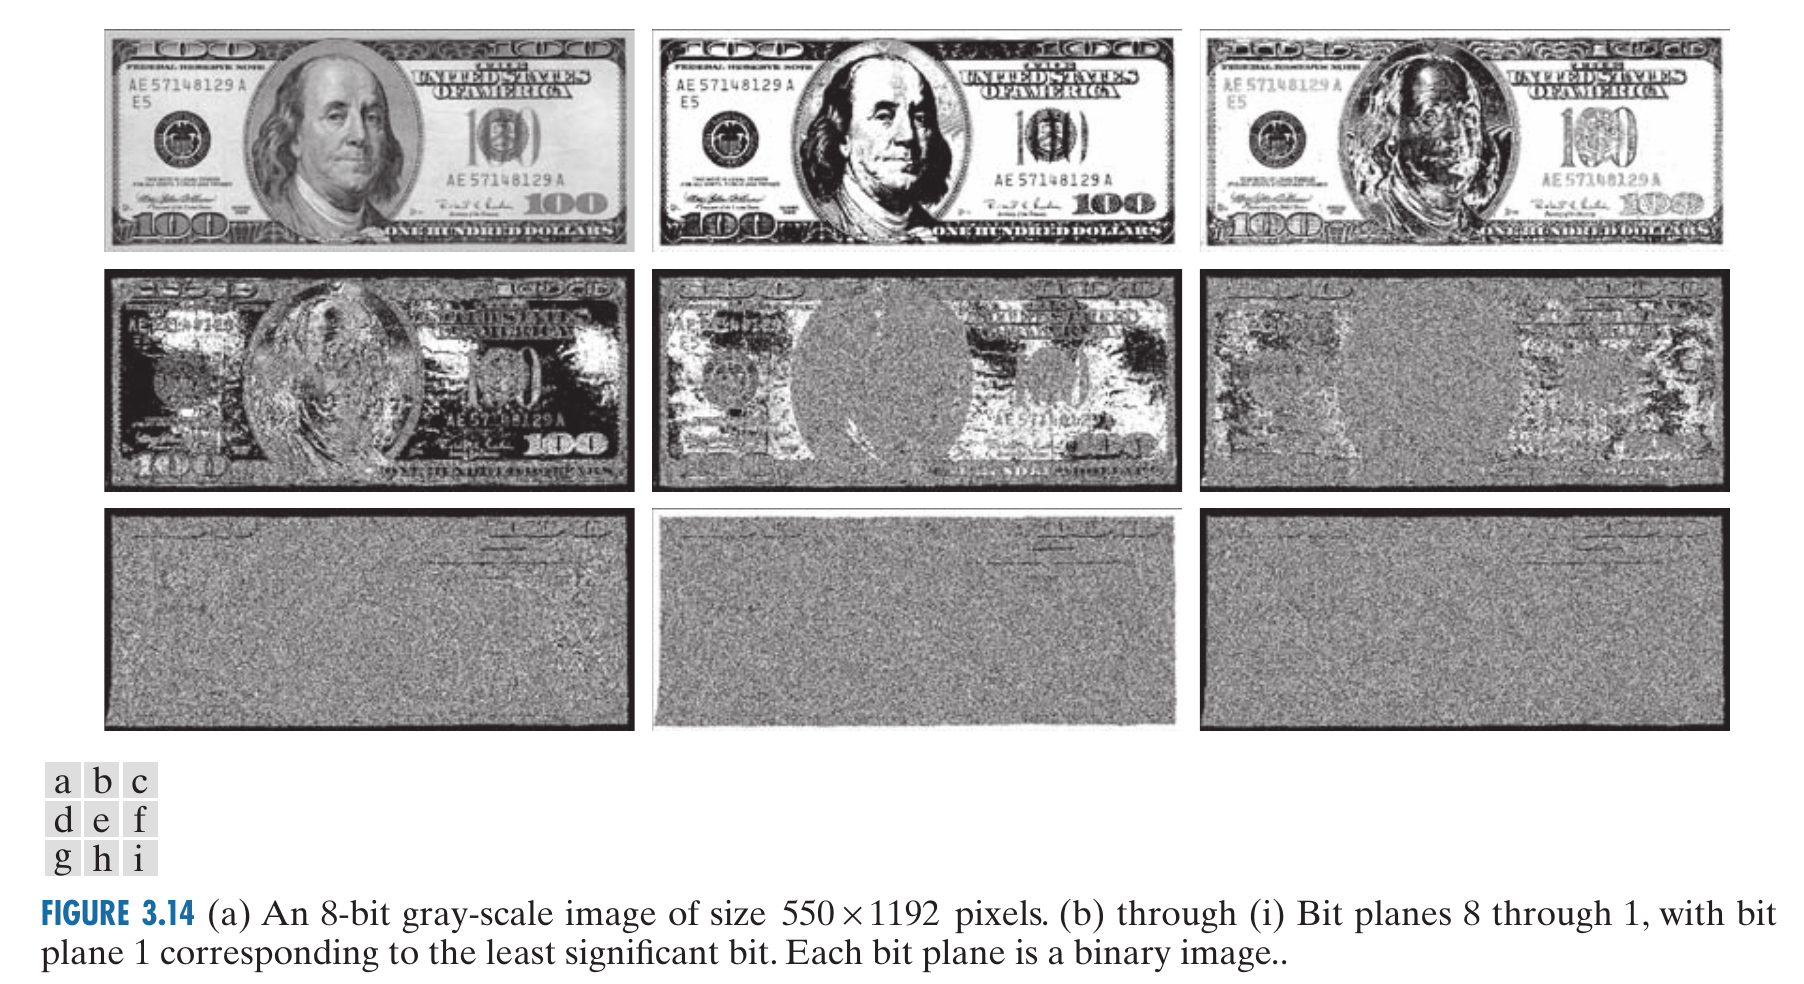
\includegraphics{img/8_bit_gray_image_bit_planes.png}}
  
  \ 
\end{frame}}{\begin{frame}
  \
  
  \
  
  \
  
  \resizebox{1\columnwidth}{!}{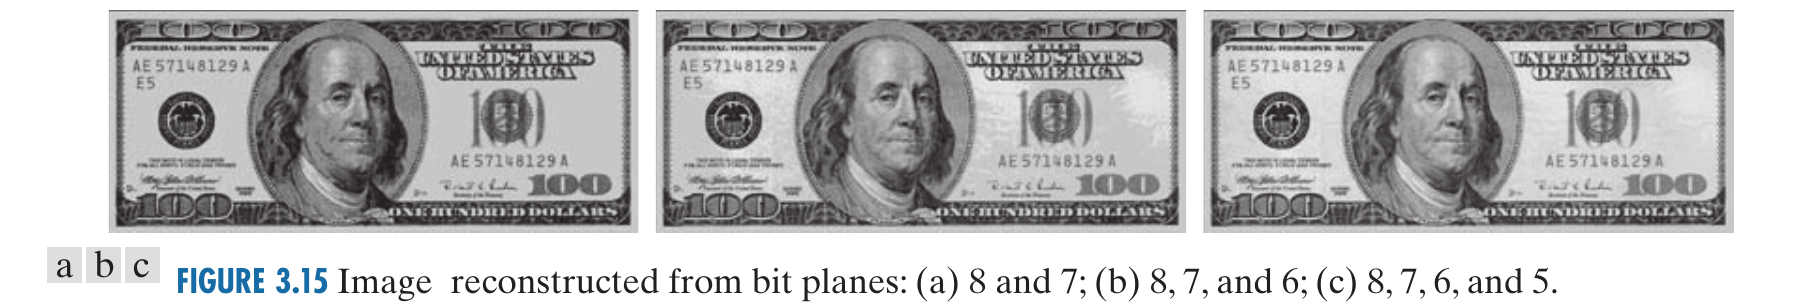
\includegraphics{img/bit_planes_reconstruct.png}}
\end{frame}}{\begin{frame}
  \frametitle{直方图}
  
  \resizebox{1\columnwidth}{!}{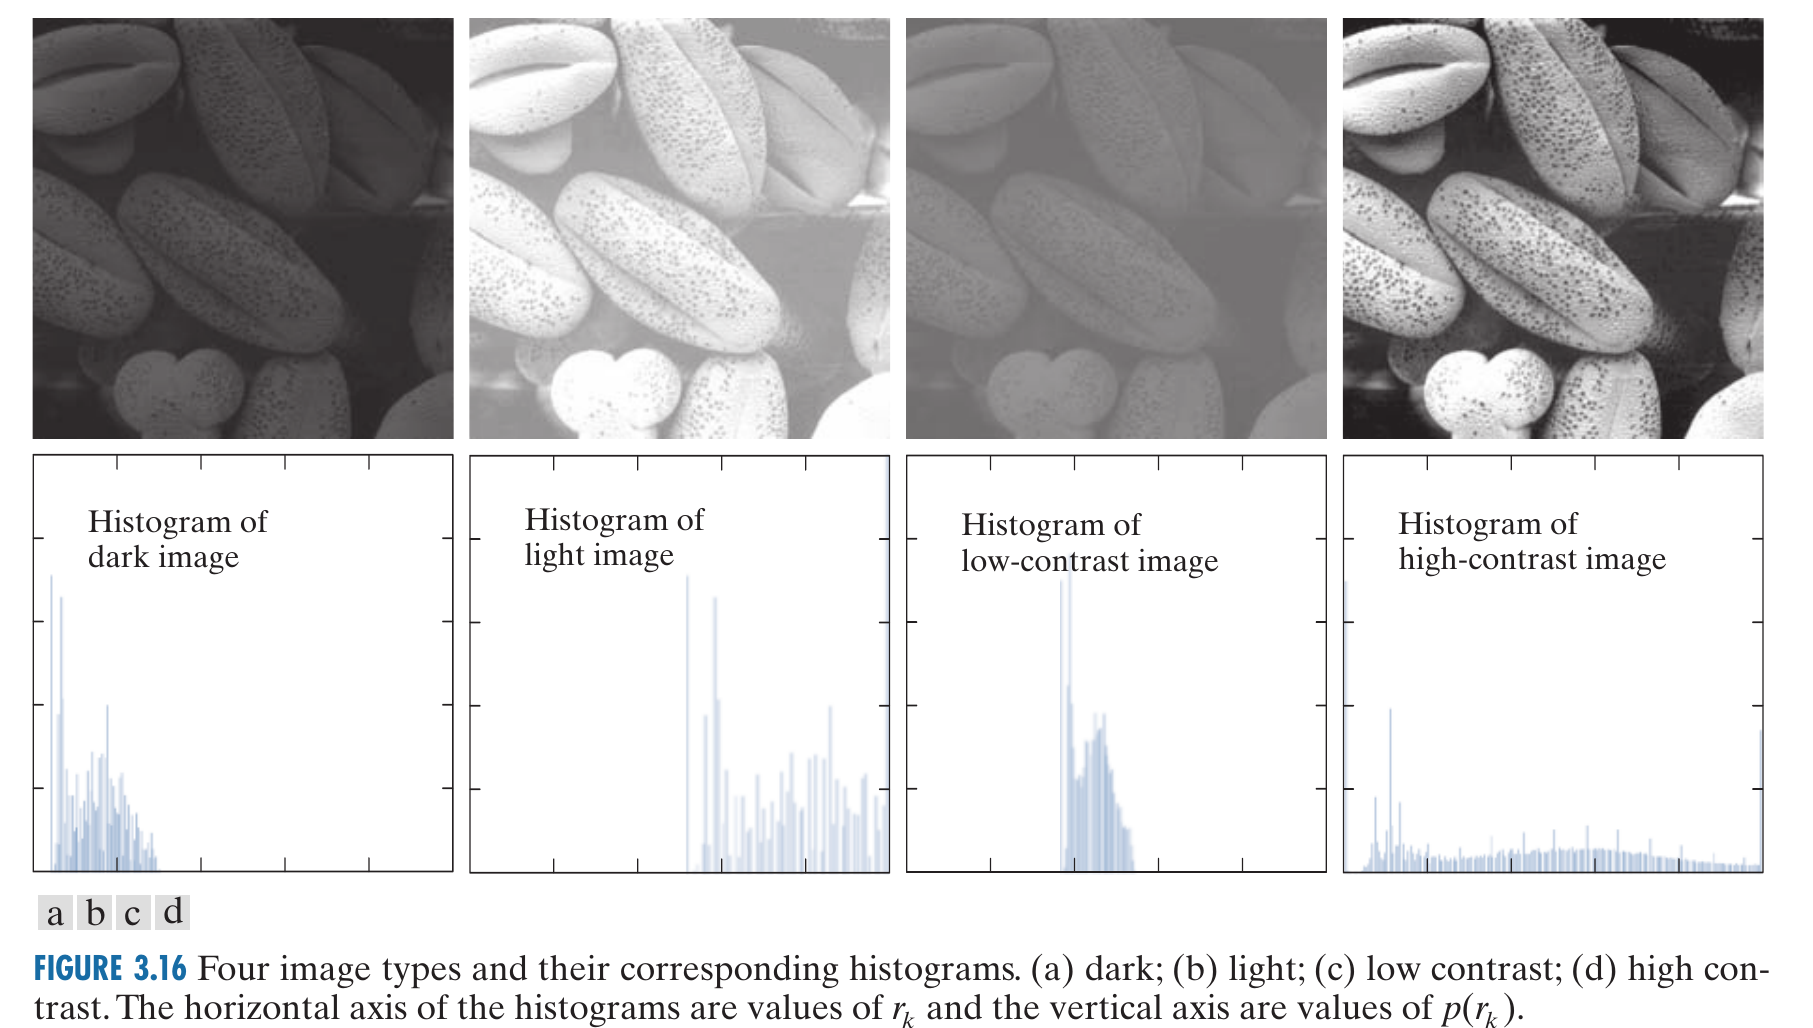
\includegraphics{img/histogram.png}}\label{4_image_histograms}
\end{frame}}{\begin{frame}
  \frametitle{直方图均衡}
  \begin{eqnarray*}
    s & = & g (r)\\
    p (s) \mathd s & = & p (r) \mathd r\\
    \frac{1}{L} \mathd s & = & p (r) \mathd r\\
    \frac{\mathd s}{\mathd r} & = & L \nospace p (r)\\
    s & = & L \int_0^r p (x) \mathd x
  \end{eqnarray*}
  $\label{histogram-equalization}$
\end{frame}}{\begin{frame}
  \frametitle{单增函数}
  
  \resizebox{1\columnwidth}{!}{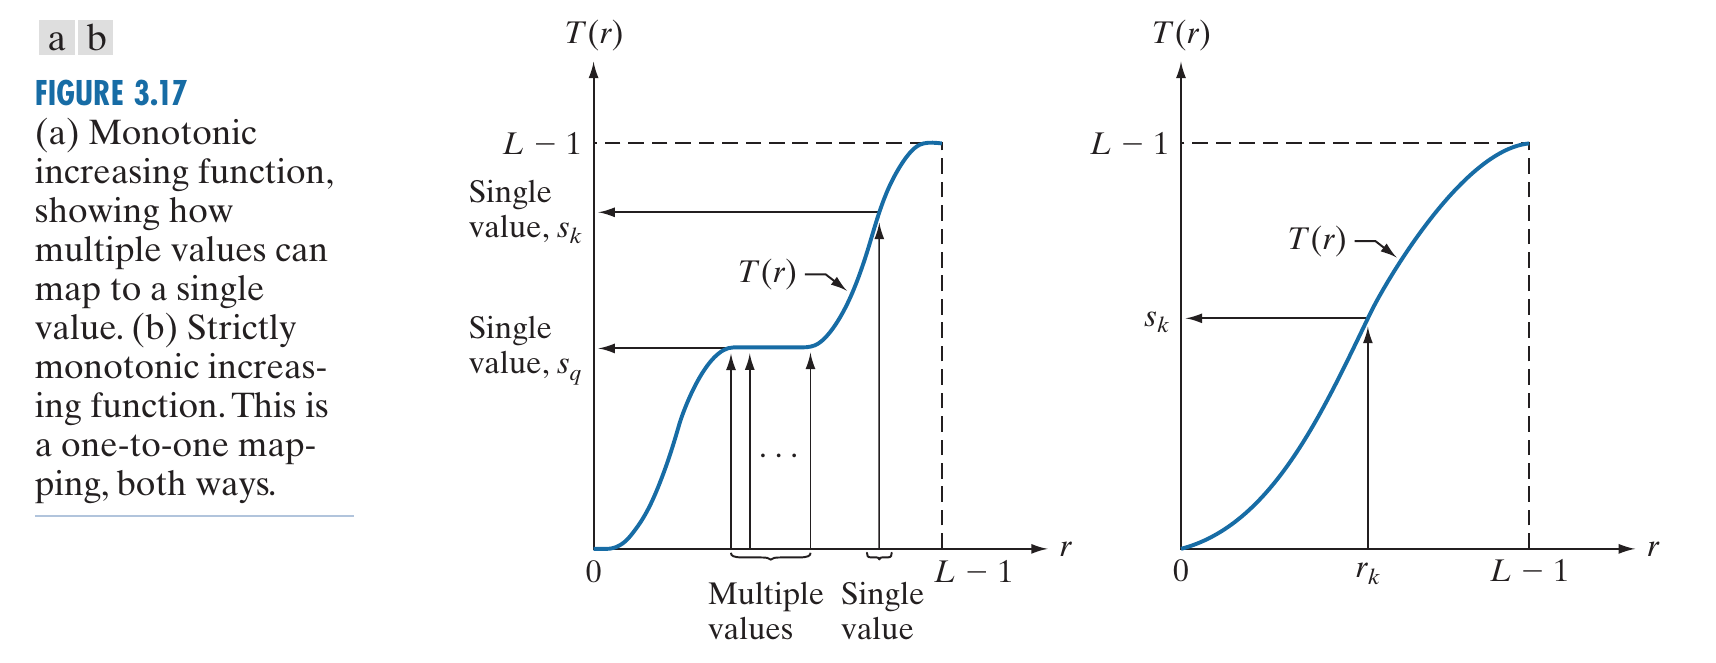
\includegraphics{img/monotonic_increasing_function.png}}
\end{frame}}{\begin{frame}
  \frametitle{概率分布变换}
  
  \resizebox{1\columnwidth}{!}{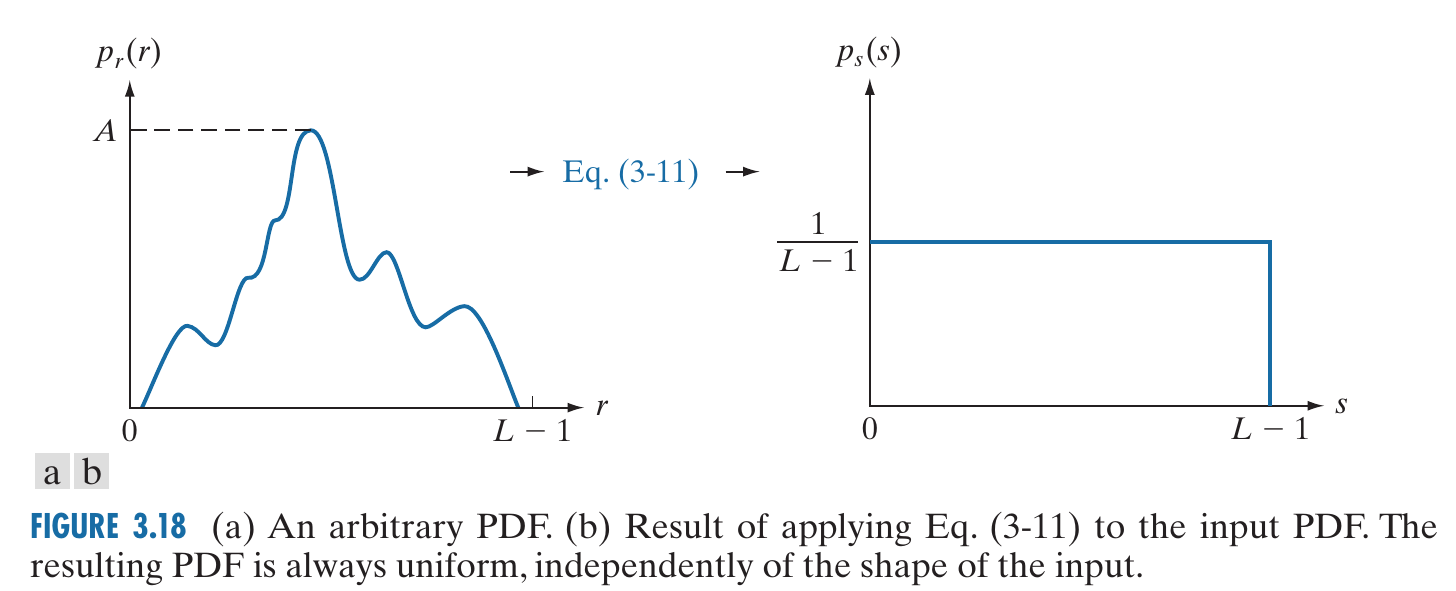
\includegraphics{img/PDF_to_uniform.png}}
\end{frame}}{\begin{frame}
  \frametitle{直方图变换示例}
  
  \
  
  \
  
  \resizebox{1\columnwidth}{!}{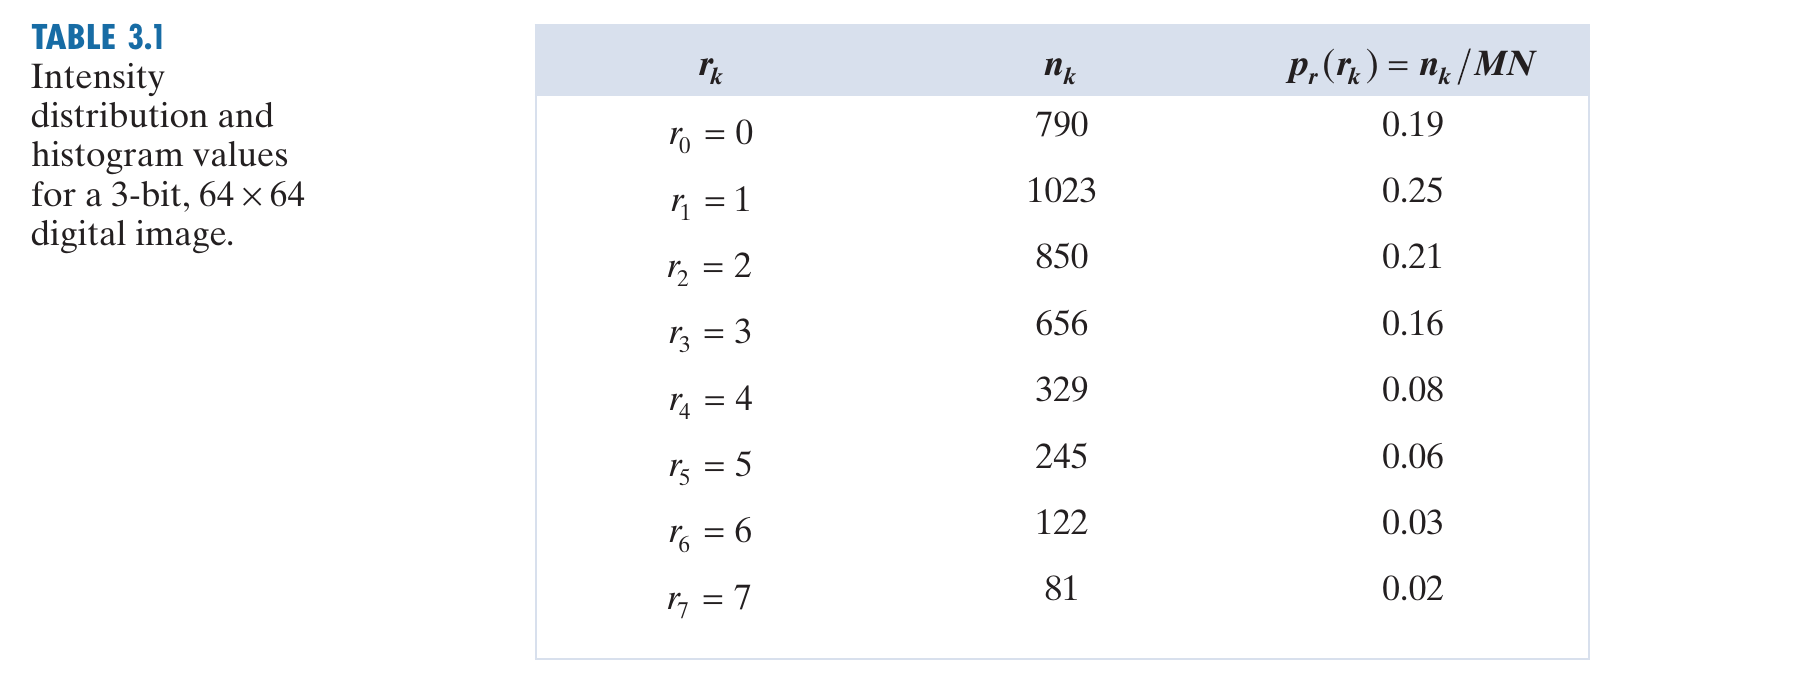
\includegraphics{img/histogram_equalization_3_bit_image.png}}
\end{frame}}{\begin{frame}
  \frametitle{直方图变换示例(续)}
  
  \
  
  \
  
  \
  
  \resizebox{1\columnwidth}{!}{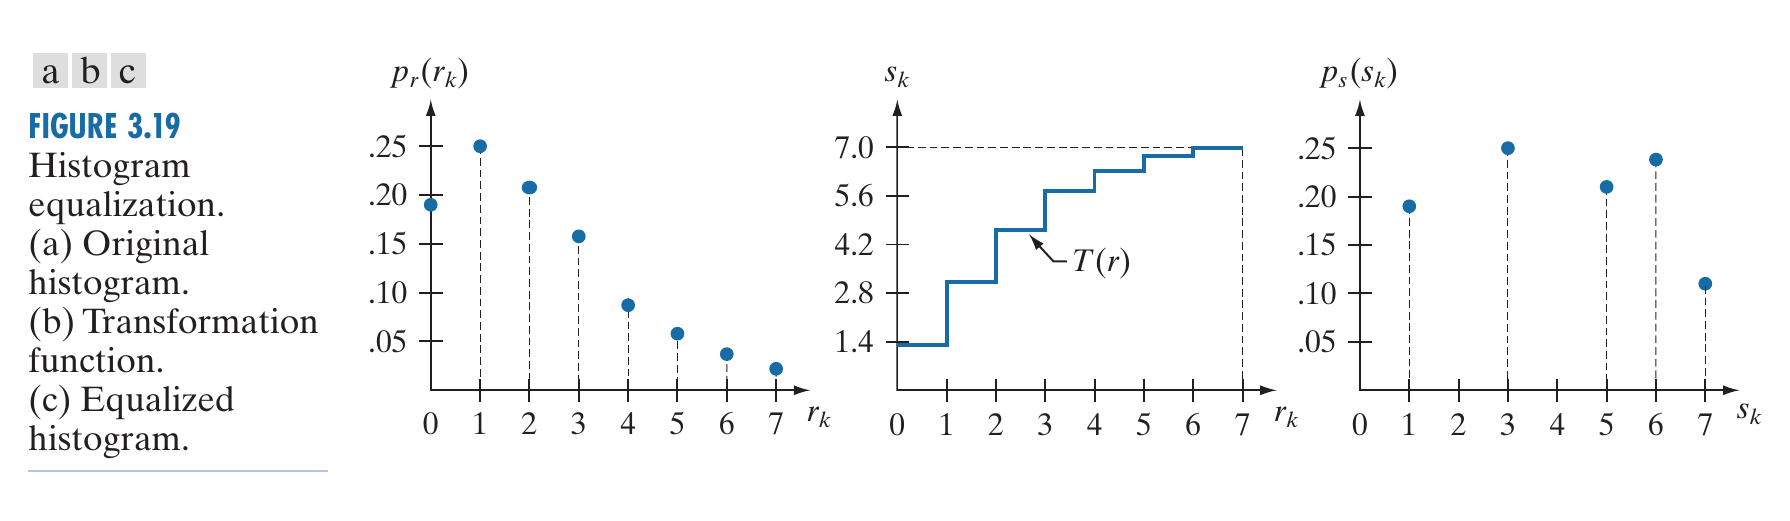
\includegraphics{img/histogram_equalization.png}}
\end{frame}}{\begin{frame}
  {\hspace{5em}}\resizebox{0.6\columnwidth}{!}{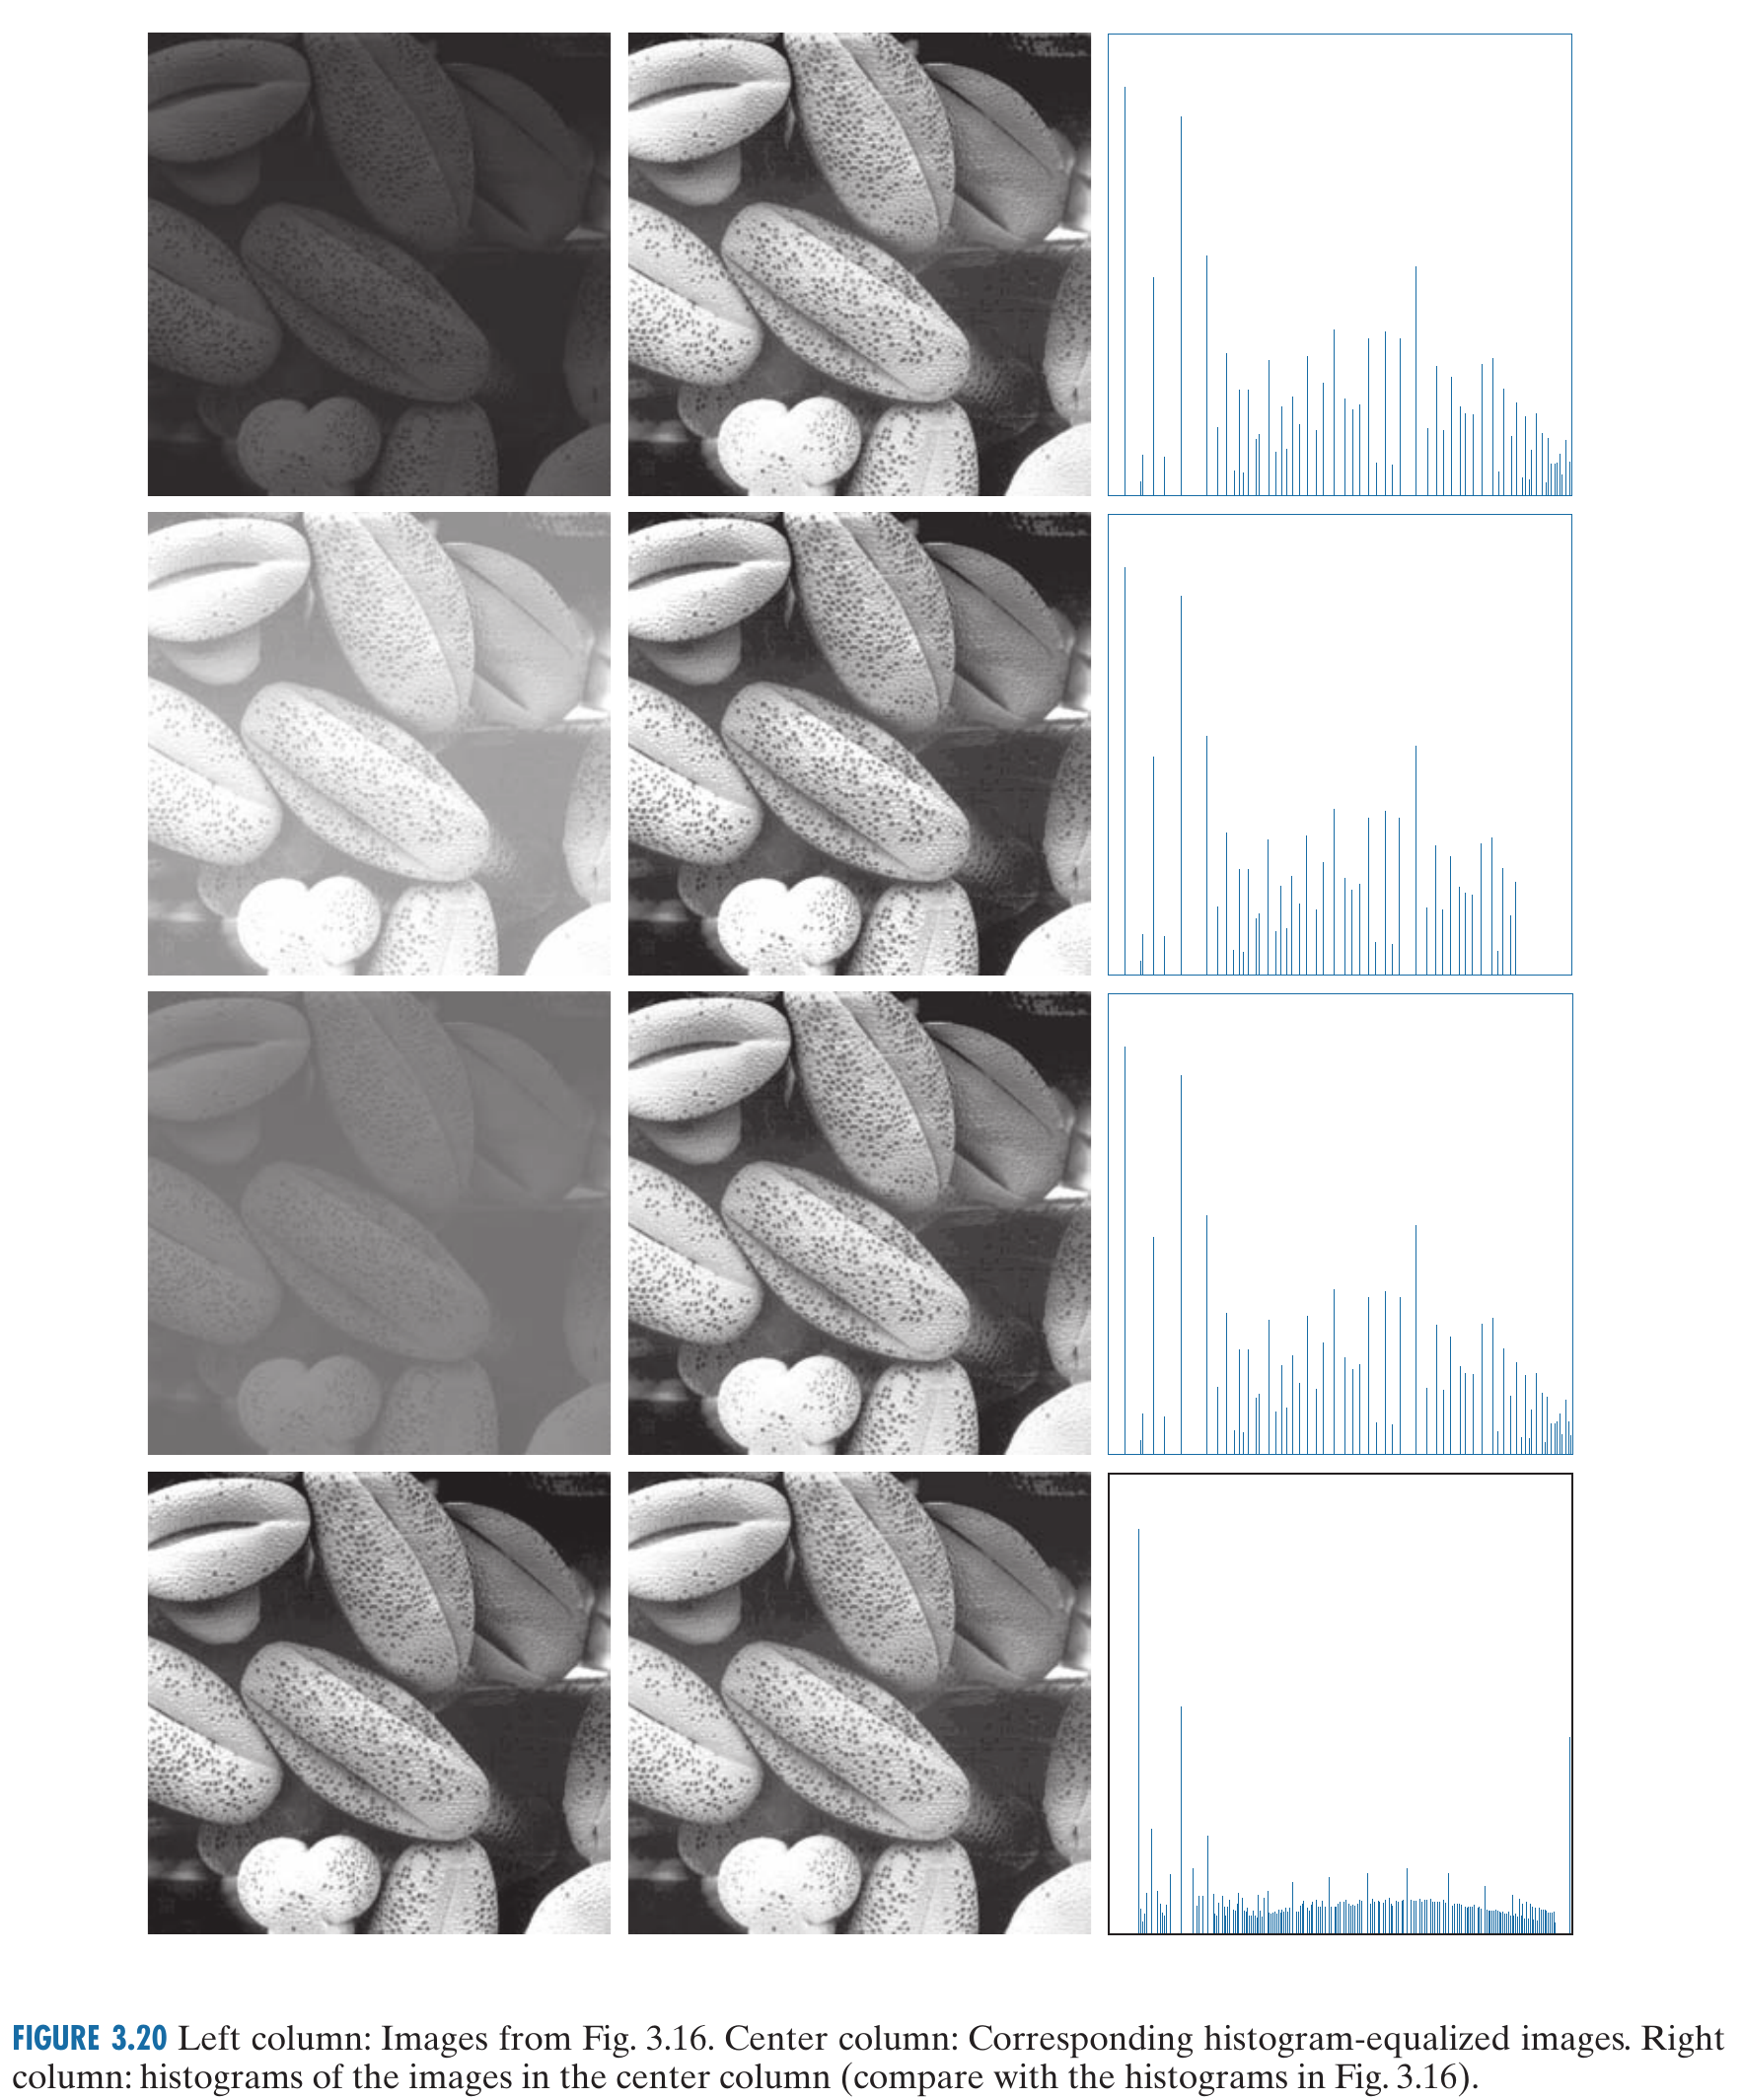
\includegraphics{img/image_histogram_equalization.png}}\hyperref[4_image_histograms]{\^{}.
  \^{}}
\end{frame}}{\begin{frame}
  \
  
  \
  
  \resizebox{1\columnwidth}{!}{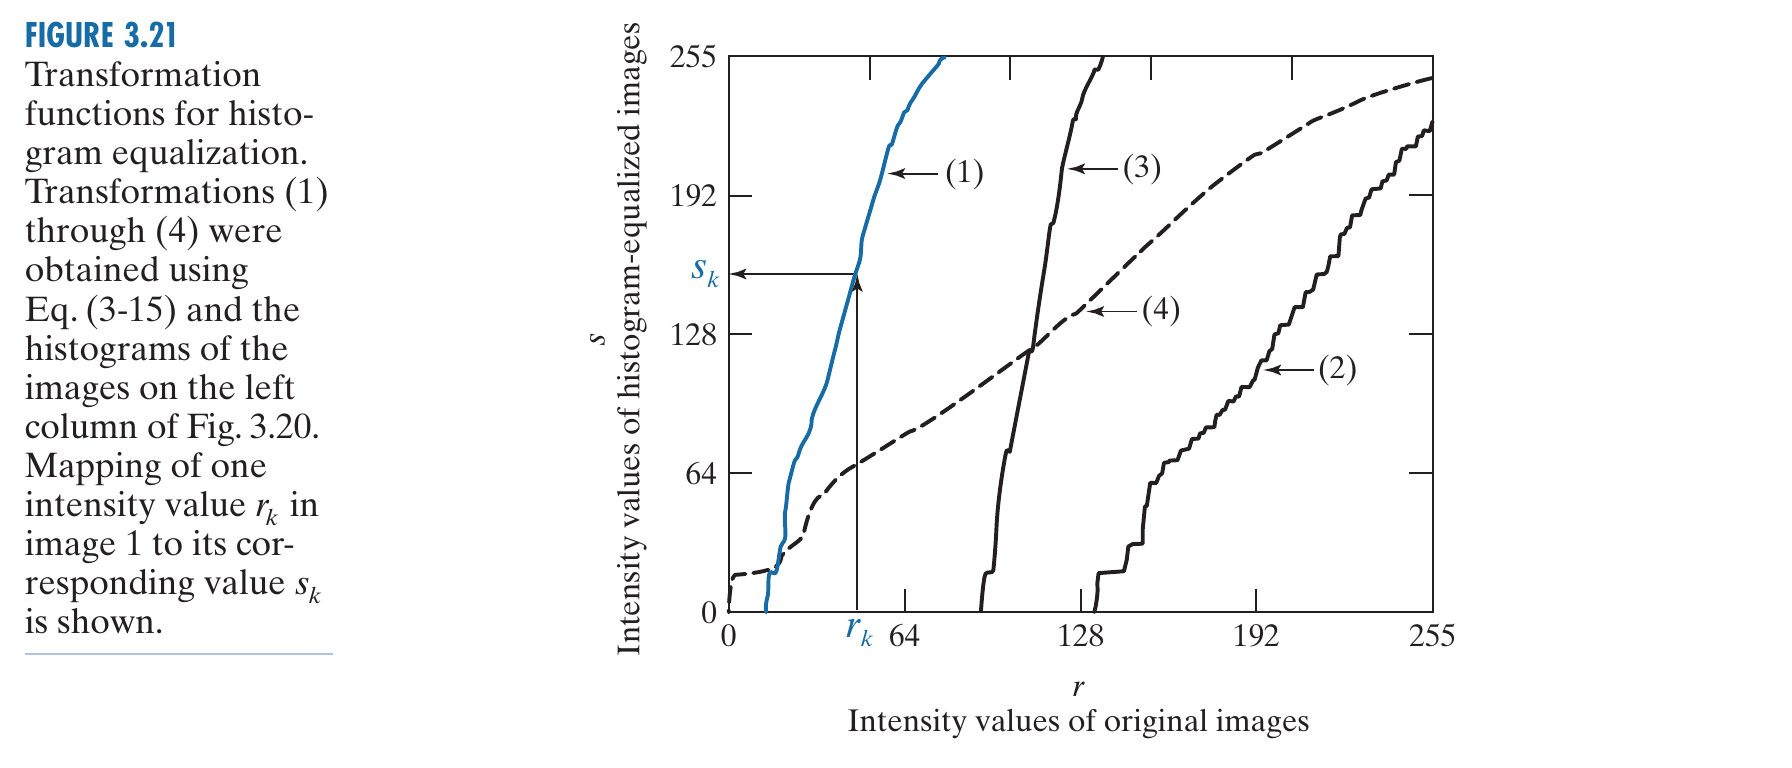
\includegraphics{img/image_histogram_equalization_transformation_function.png}}
  
  \hyperref[4_image_histograms]{\^{}. \^{}}
\end{frame}}{\begin{frame}
  \frametitle{直方图匹配(规定化)}
  
  
  \begin{eqnarray*}
    z & = & g (s)\\
    s & = & g^{- 1} (z)\\
    p (z) \mathd z & = & p (s) \mathd s\\
    p (z) \mathd z & = & \frac{1}{L} \mathd s\\
    \frac{\mathd s}{\mathd z} & = & L \nospace p (z)\\
    s & = & L \int_0^z p (x) \mathd x
  \end{eqnarray*}
  \hyperref[histogram-equalization]{\^{}.\^{}}
\end{frame}}{\begin{frame}
  \
  
  \
  
  \resizebox{1\columnwidth}{!}{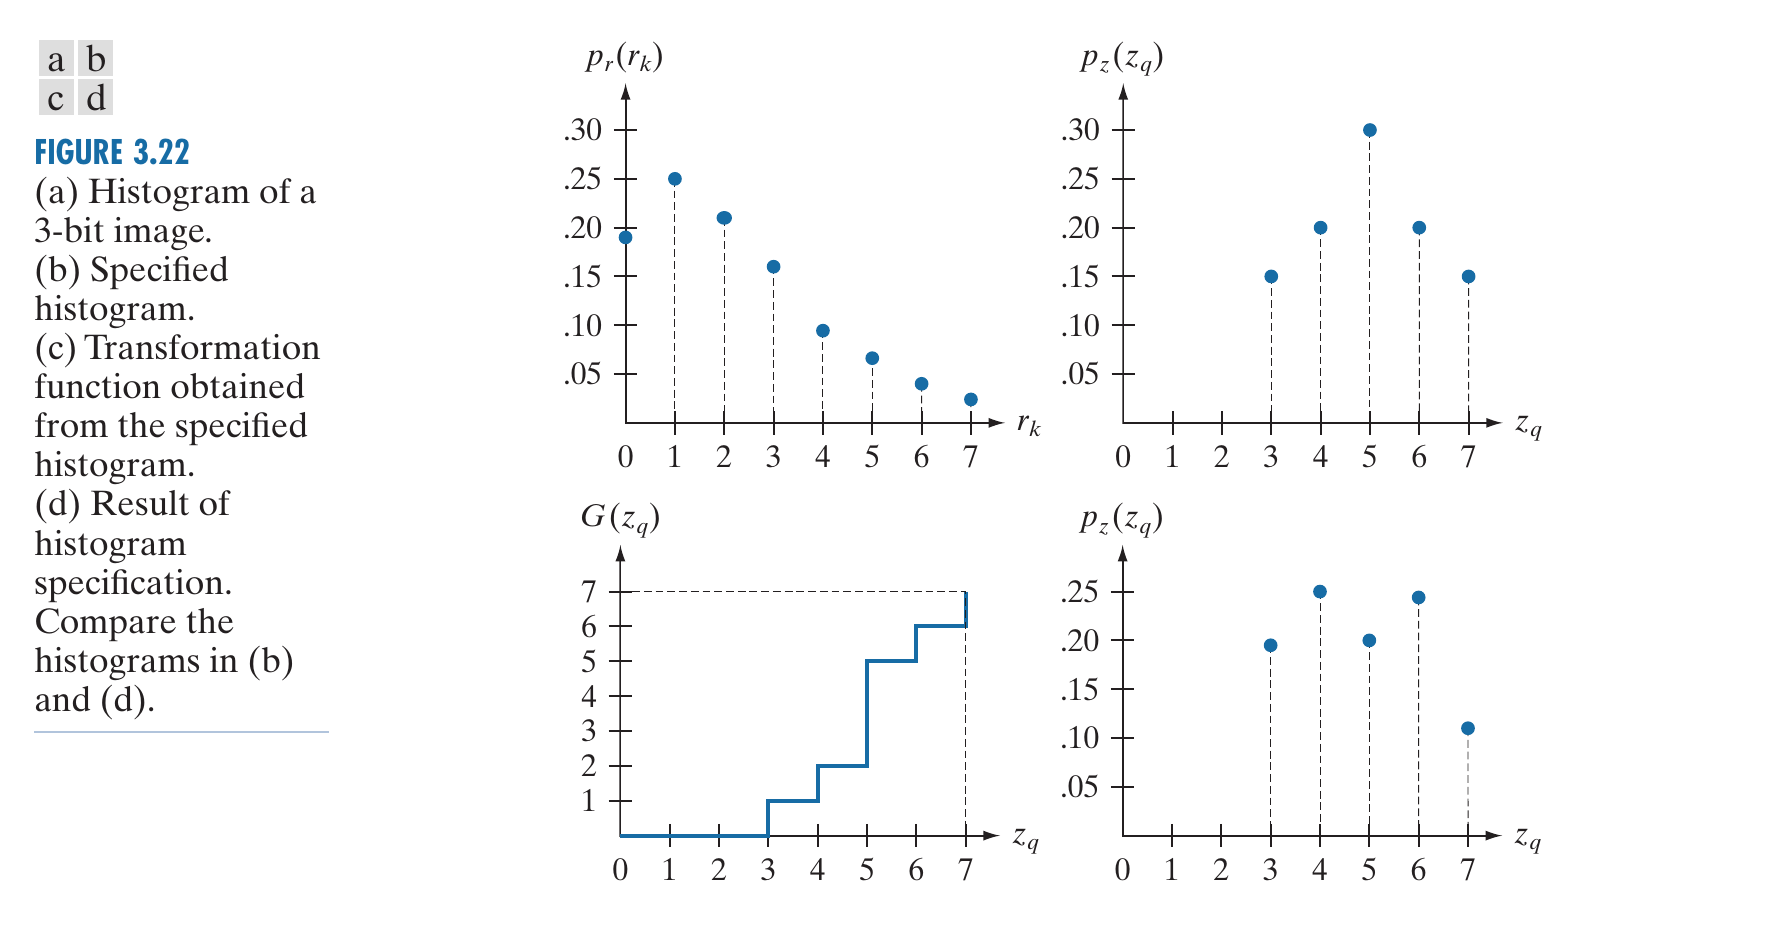
\includegraphics{img/histogram_specification_3_bit_image.png}}
\end{frame}}{\begin{frame}
  \
  
  \
  
  \tmfoldedstd{\resizebox{1\columnwidth}{!}{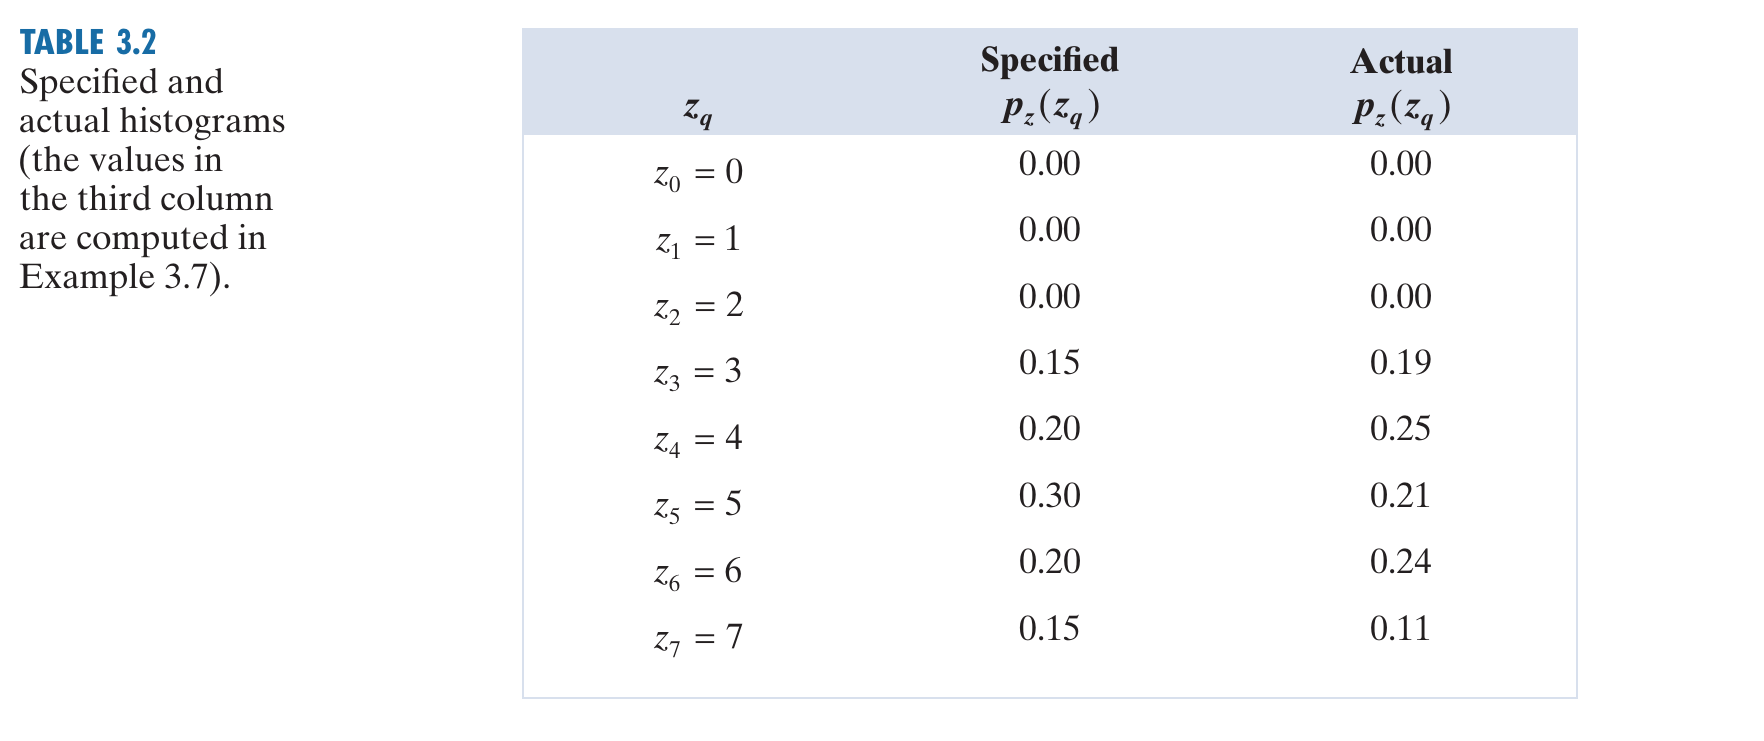
\includegraphics{img/histogram_specification_result.png}}}{\resizebox{1\columnwidth}{!}{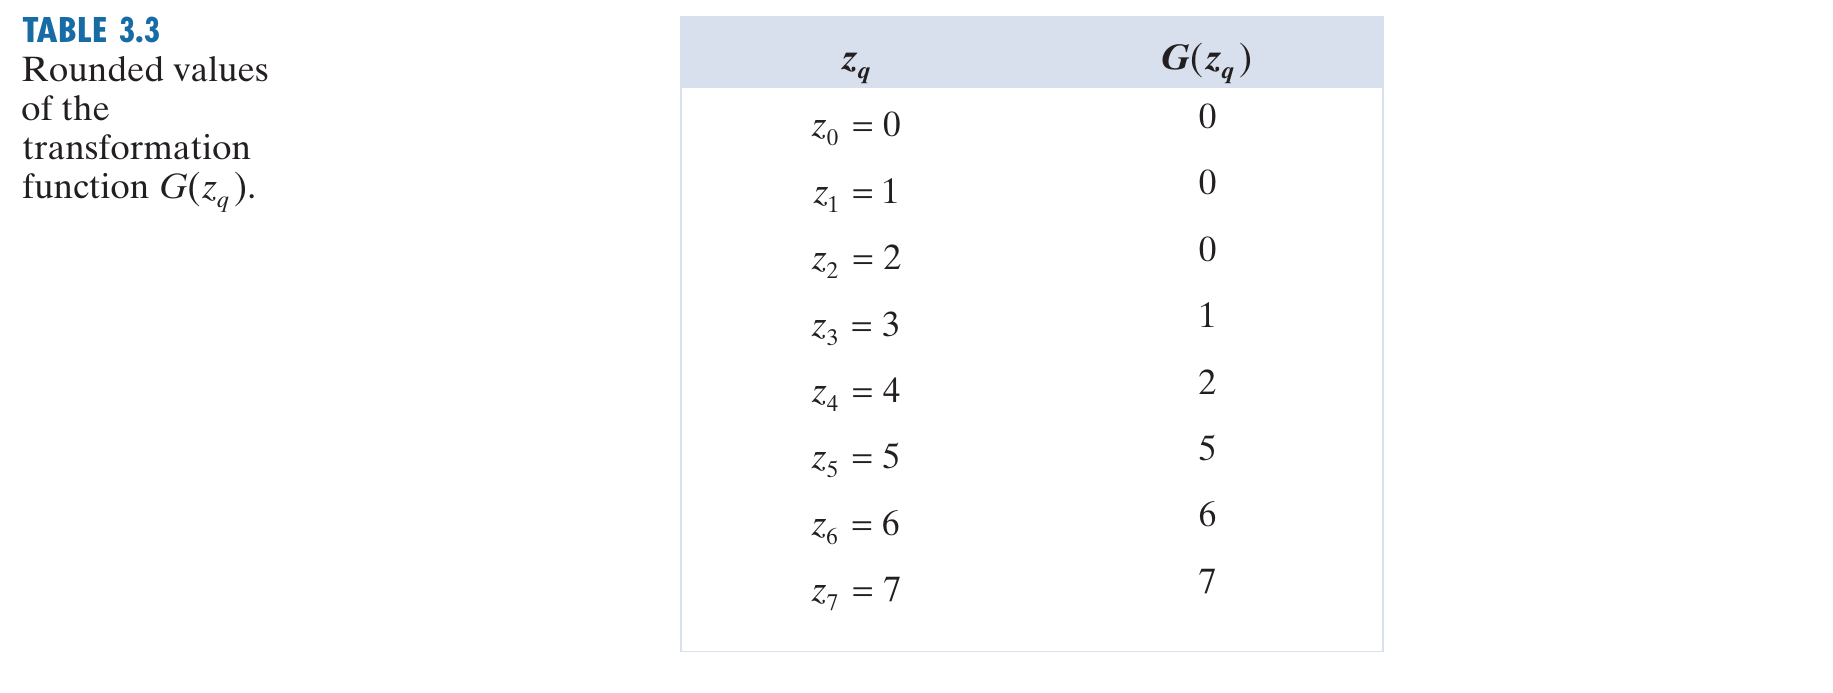
\includegraphics{img/histogram_specification_rounded_transformation_function.png}}
  
  \resizebox{1\columnwidth}{!}{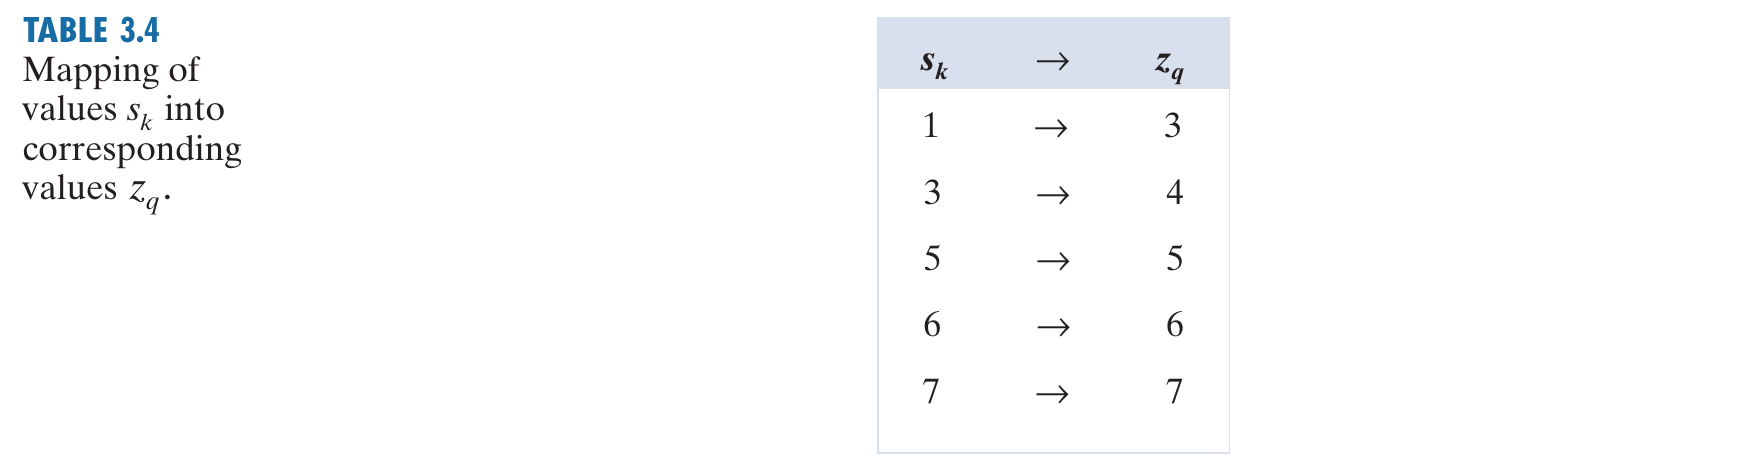
\includegraphics{img/histogram_specification_mapping_sk_zq.png}}}
  
  \ 
\end{frame}}{\begin{frame}
  \frametitle{直方图规定化示例}
  
  \
  
  \
  
  \resizebox{1\columnwidth}{!}{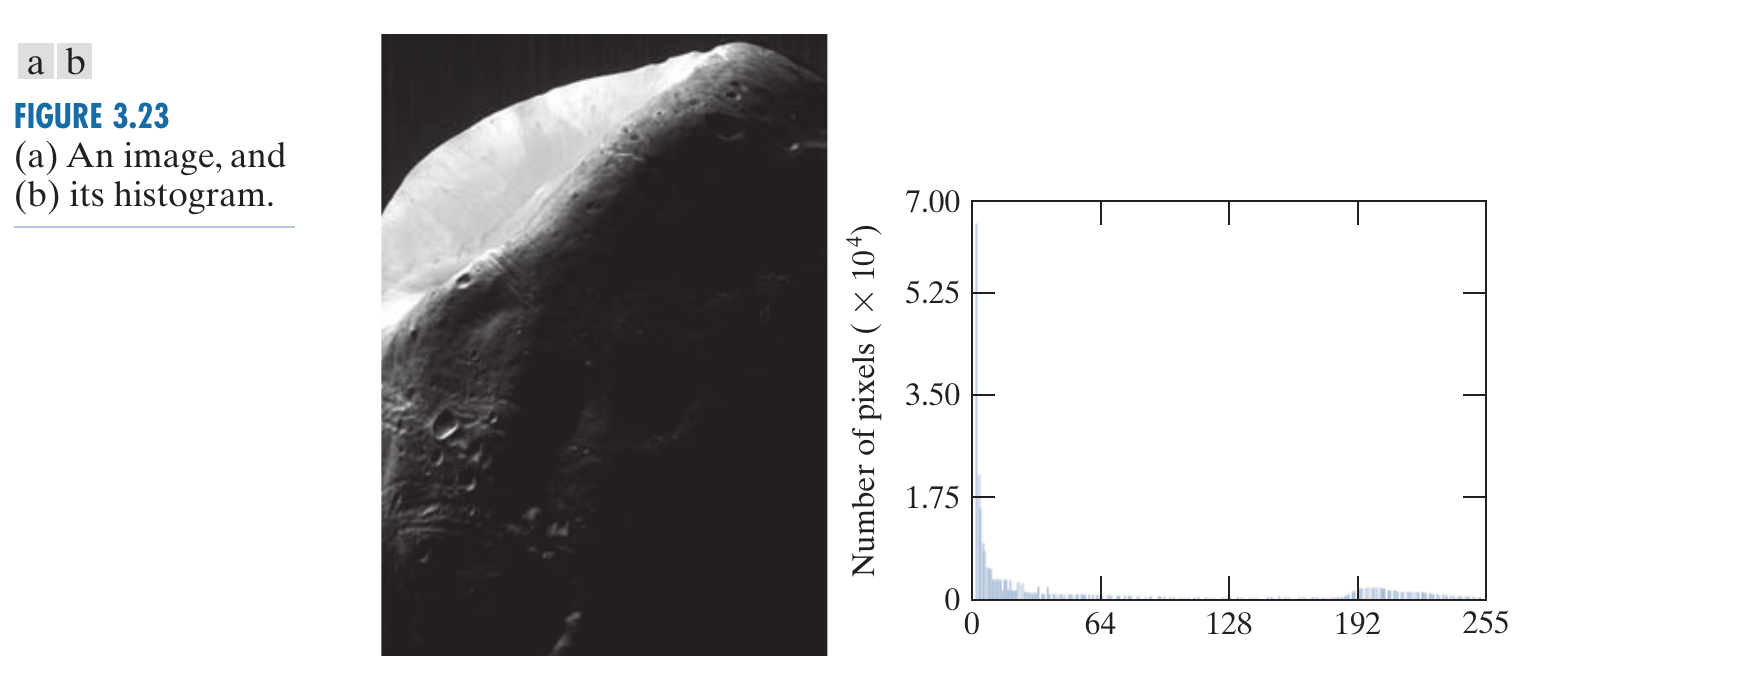
\includegraphics{img/histogram_specification_an_image_and_its_histogram.png}}
  
  \ 
\end{frame}}{\begin{frame}
  \frametitle{直方图规定化示例(续)}
  
  \resizebox{1\columnwidth}{!}{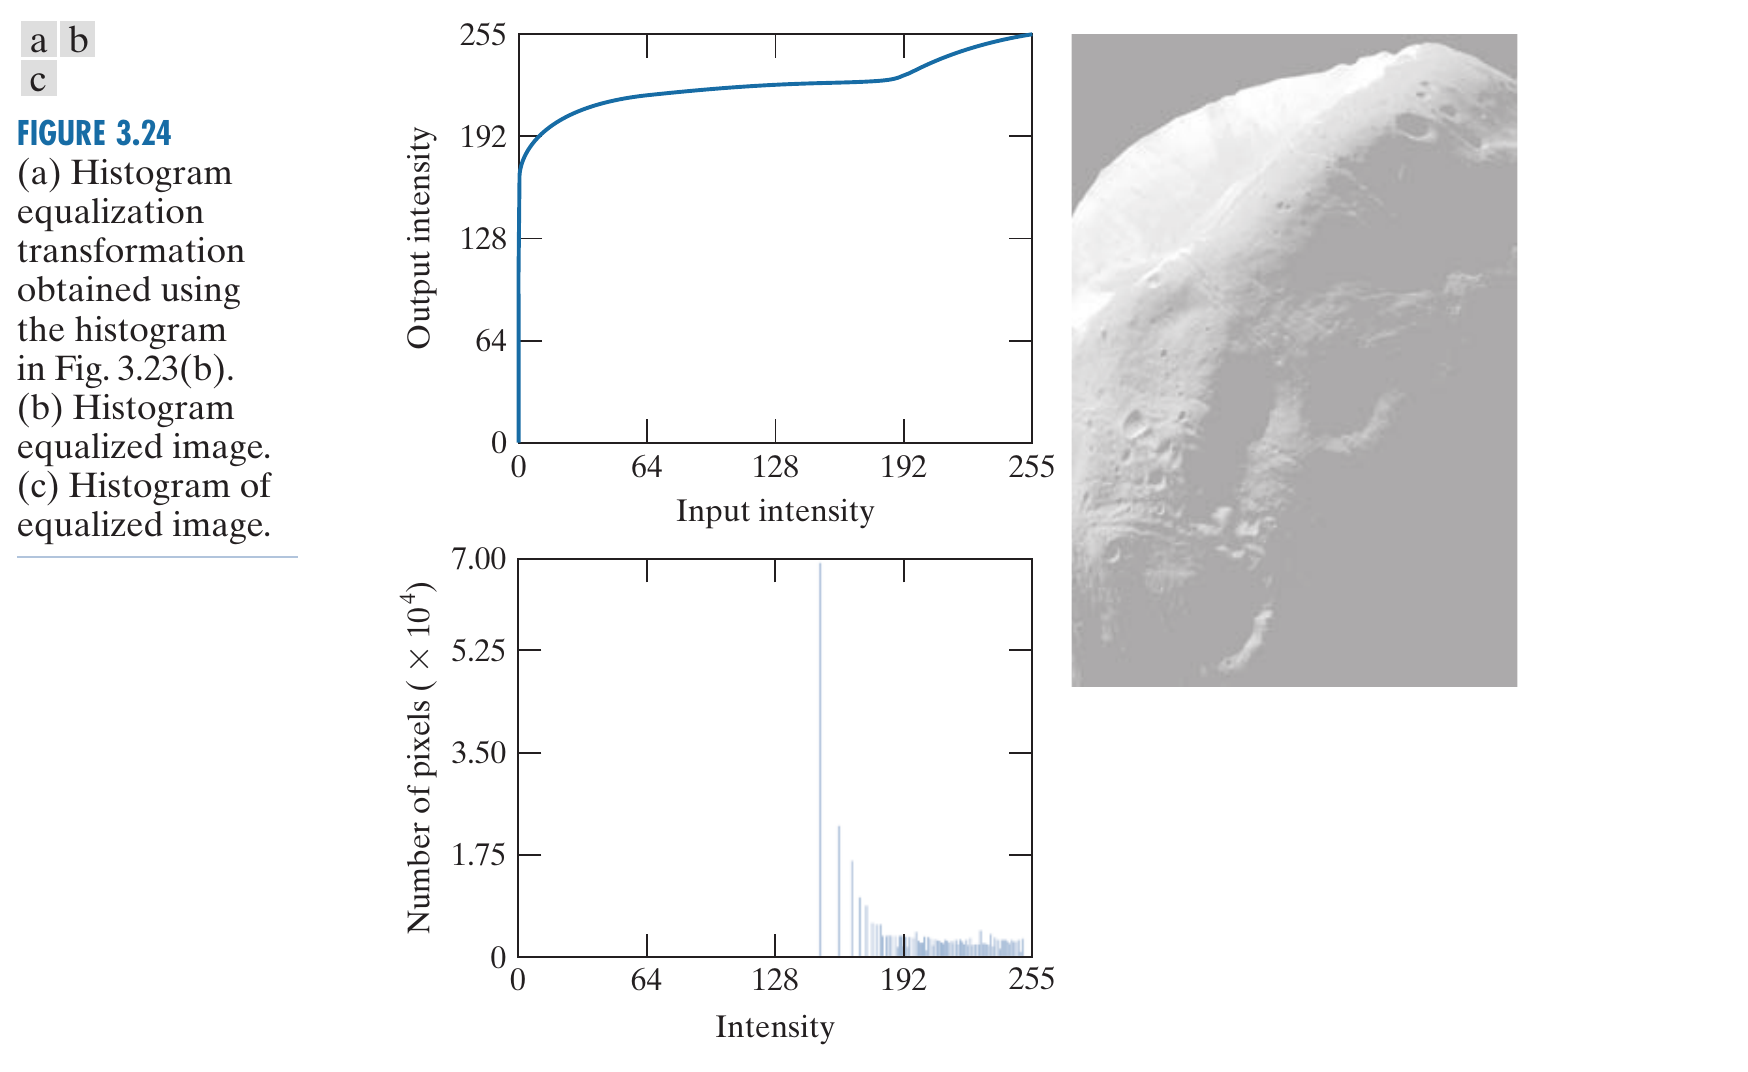
\includegraphics{img/histogram_specification_an_image__histogram_equalization.png}}
\end{frame}}{\begin{frame}
  \frametitle{直方图规定化(续)}
  
  {\hspace{5em}}\resizebox{0.6\columnwidth}{!}{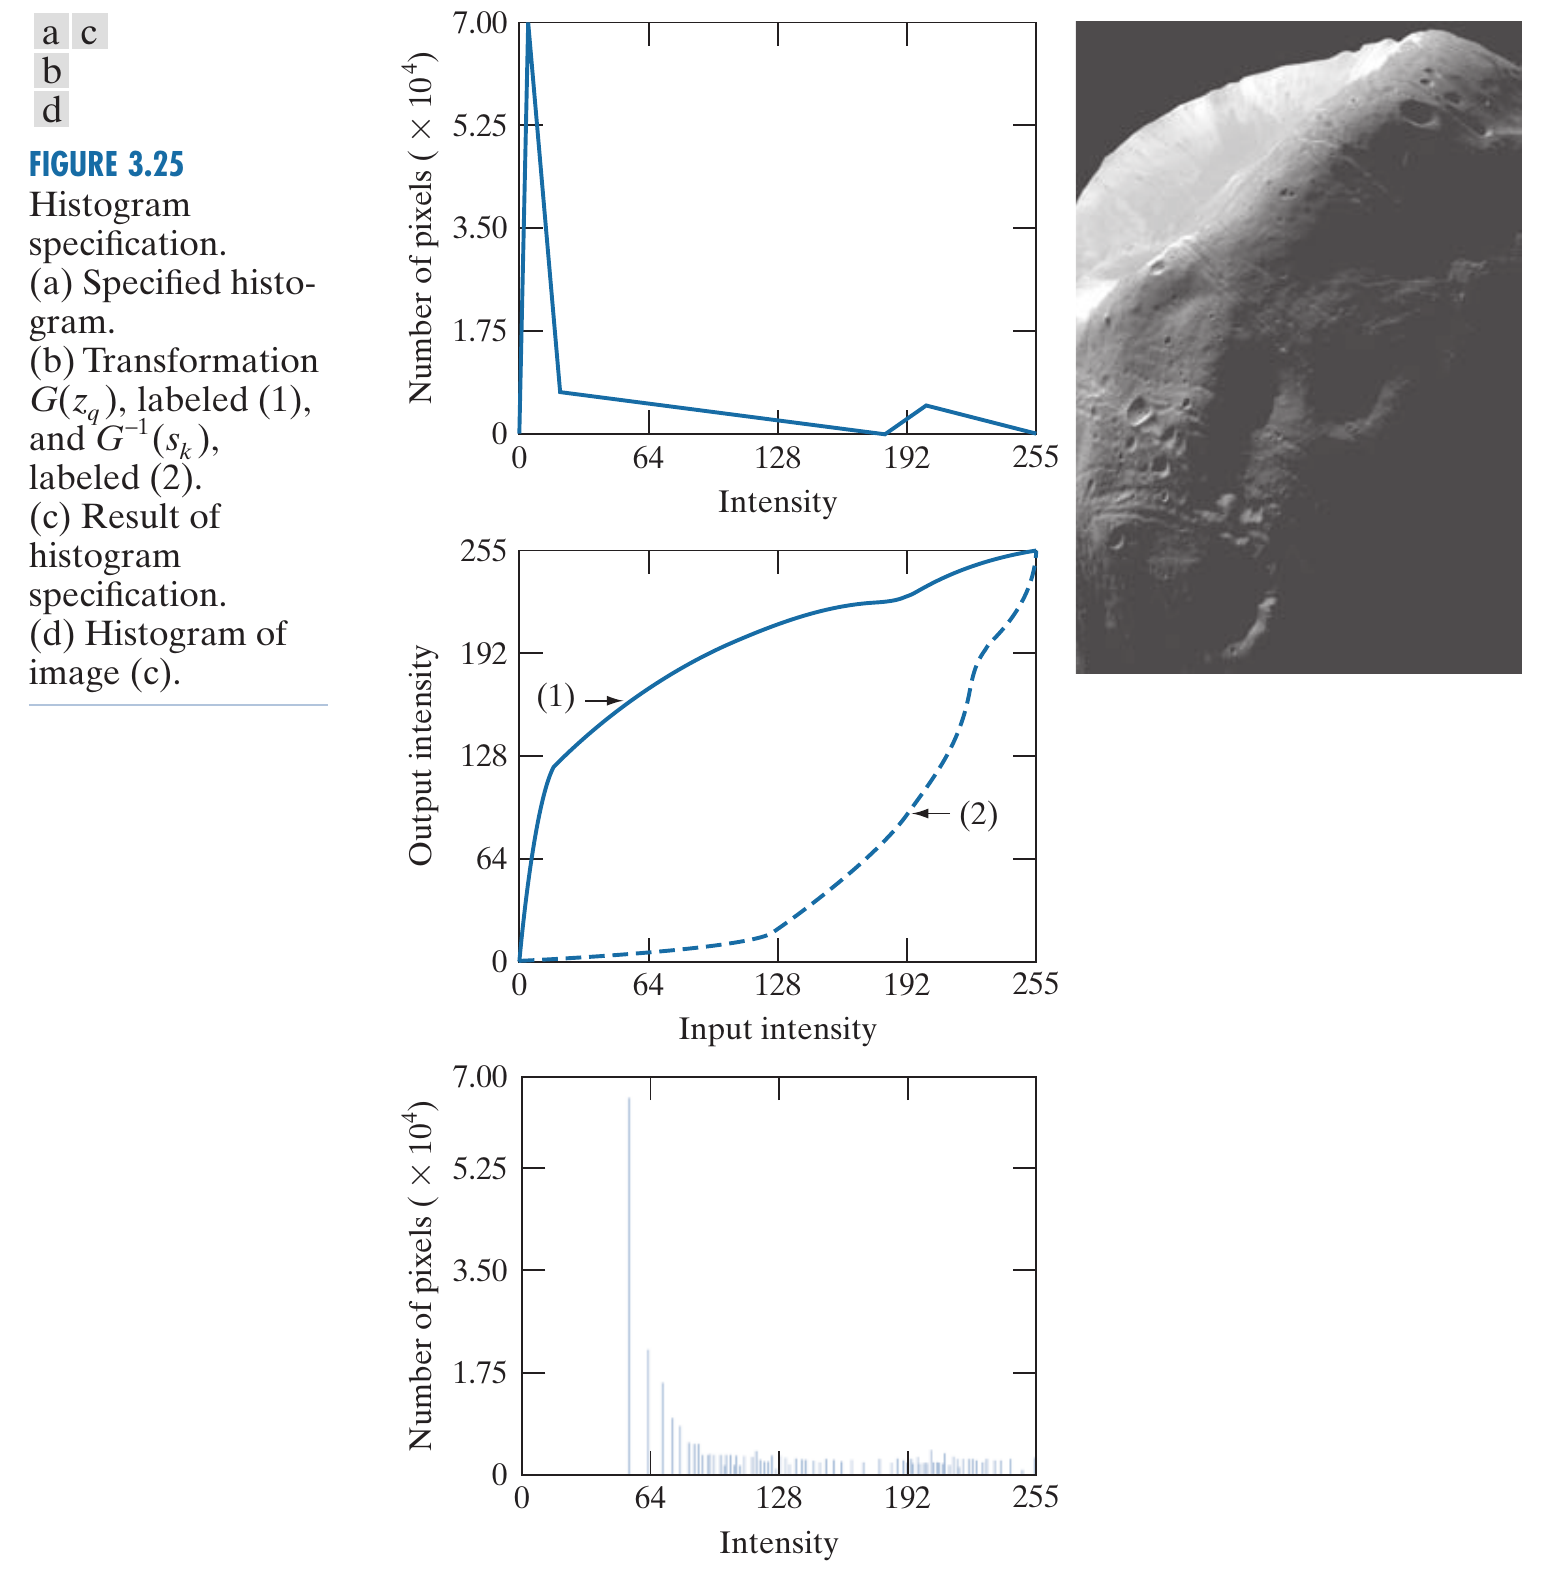
\includegraphics{img/histogram_specification_an_image__histogram_specification.png}}
\end{frame}}{\begin{frame}
  \frametitle{局部直方图均衡}
  
  \
  
  \
  
  \resizebox{1\columnwidth}{!}{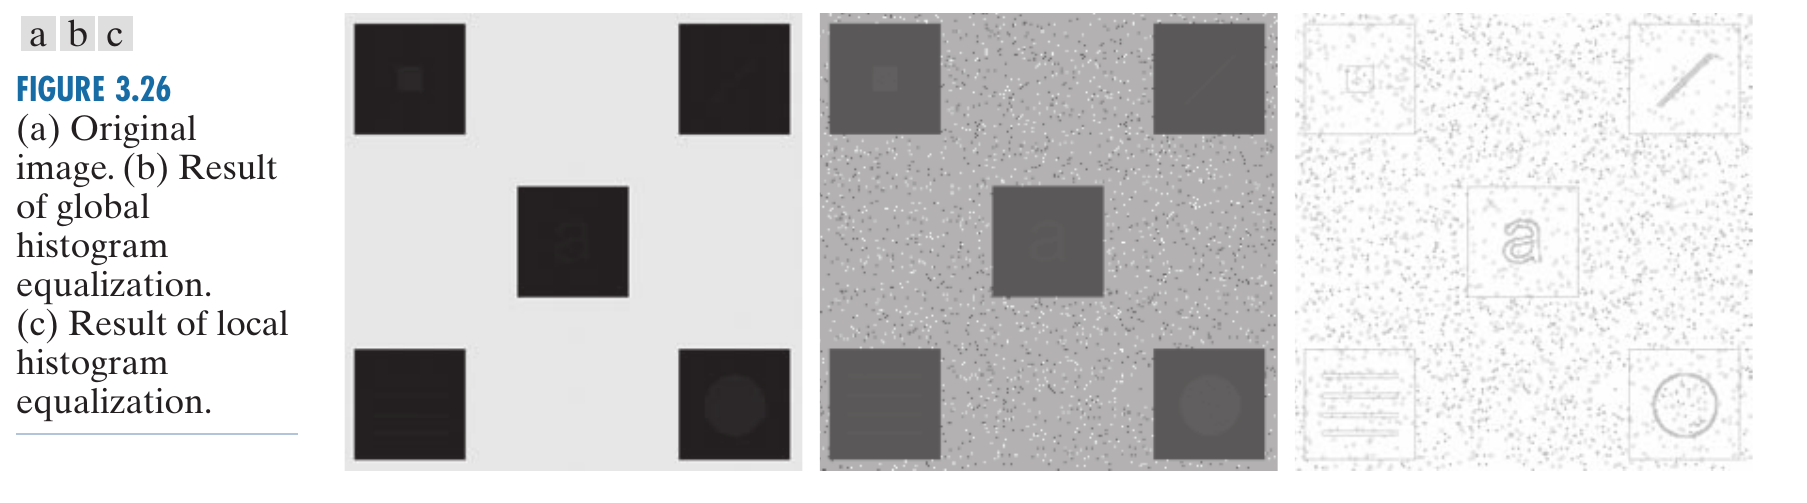
\includegraphics{img/local_histogram_equalization.png}}
\end{frame}}{\frametitle{直方图统计图像增强}


\begin{eqnarray*}
  g (x, y) & = & \left\{\begin{array}{l}
    C \nospace f (x, y)\\
    f (x, y)
  \end{array}\right. \qquad \begin{array}{l}
    k_0 m_G \leqslant m_{S_{x \nospace y}} \leqslant k_1 m_G, k_2 \sigma_G
    \leqslant \sigma_{S_{x \nospace y}} \leqslant k_3 \sigma_G\\
    \text{otherwise}
  \end{array}
\end{eqnarray*}
\resizebox{1\columnwidth}{!}{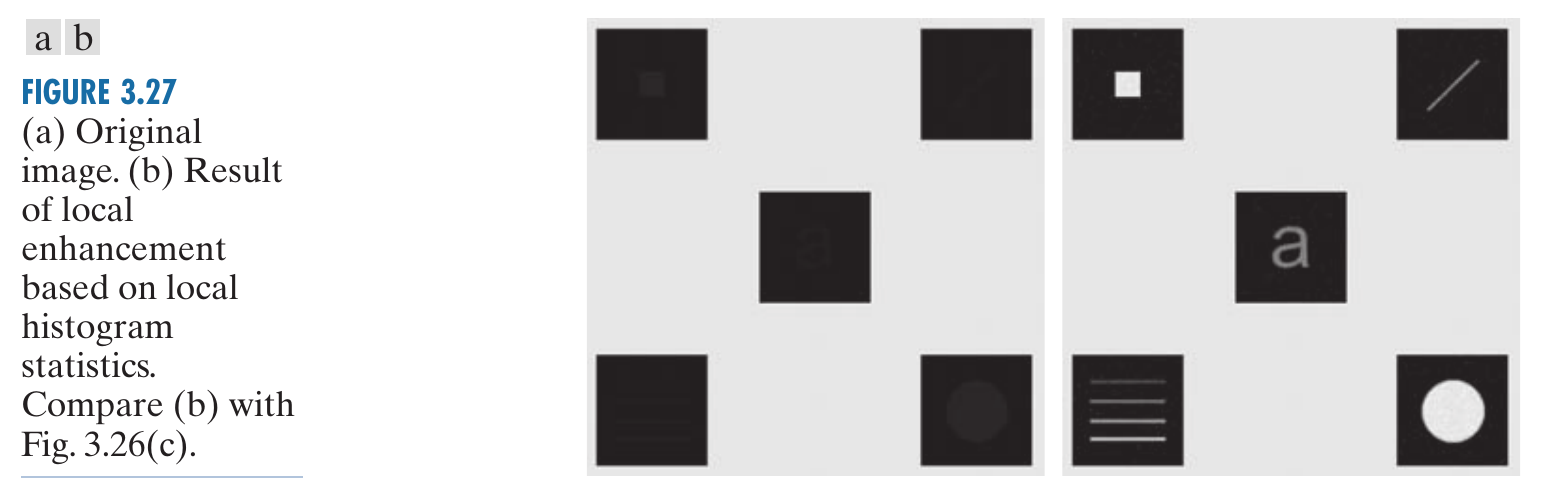
\includegraphics{img/local_histogram_statistics_enhancement.png}}}{\begin{frame}
  \frametitle{邻域}
  
  \resizebox{1\columnwidth}{!}{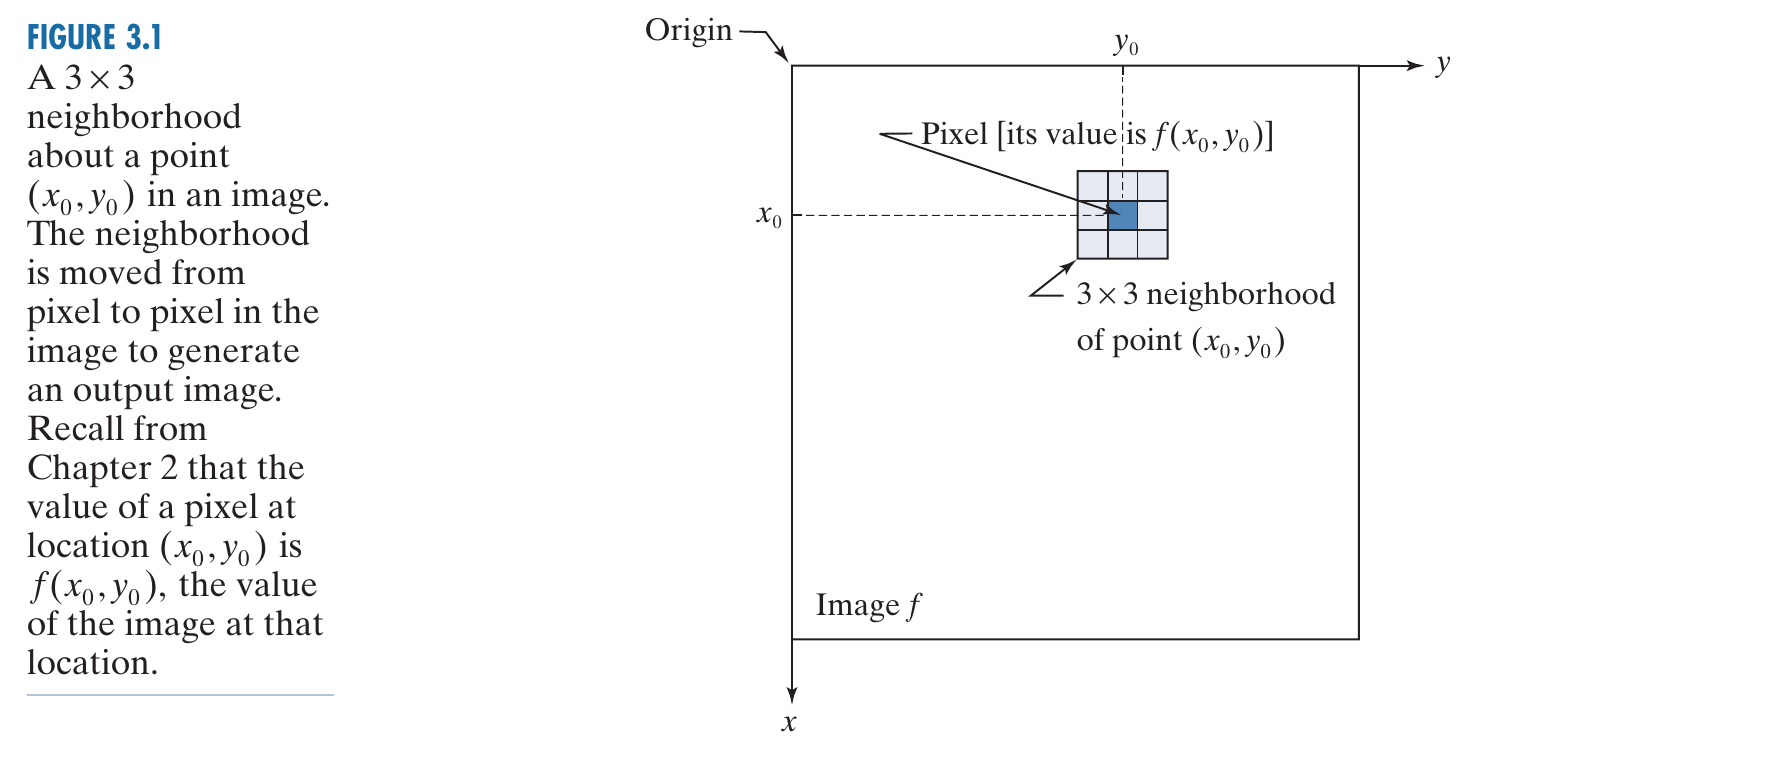
\includegraphics{img/3_3_neighborhood.png}}
\end{frame}}{\begin{frame}
  \frametitle{空间相关与卷积}
  
  {\hspace{4em}}\resizebox{0.7\columnwidth}{!}{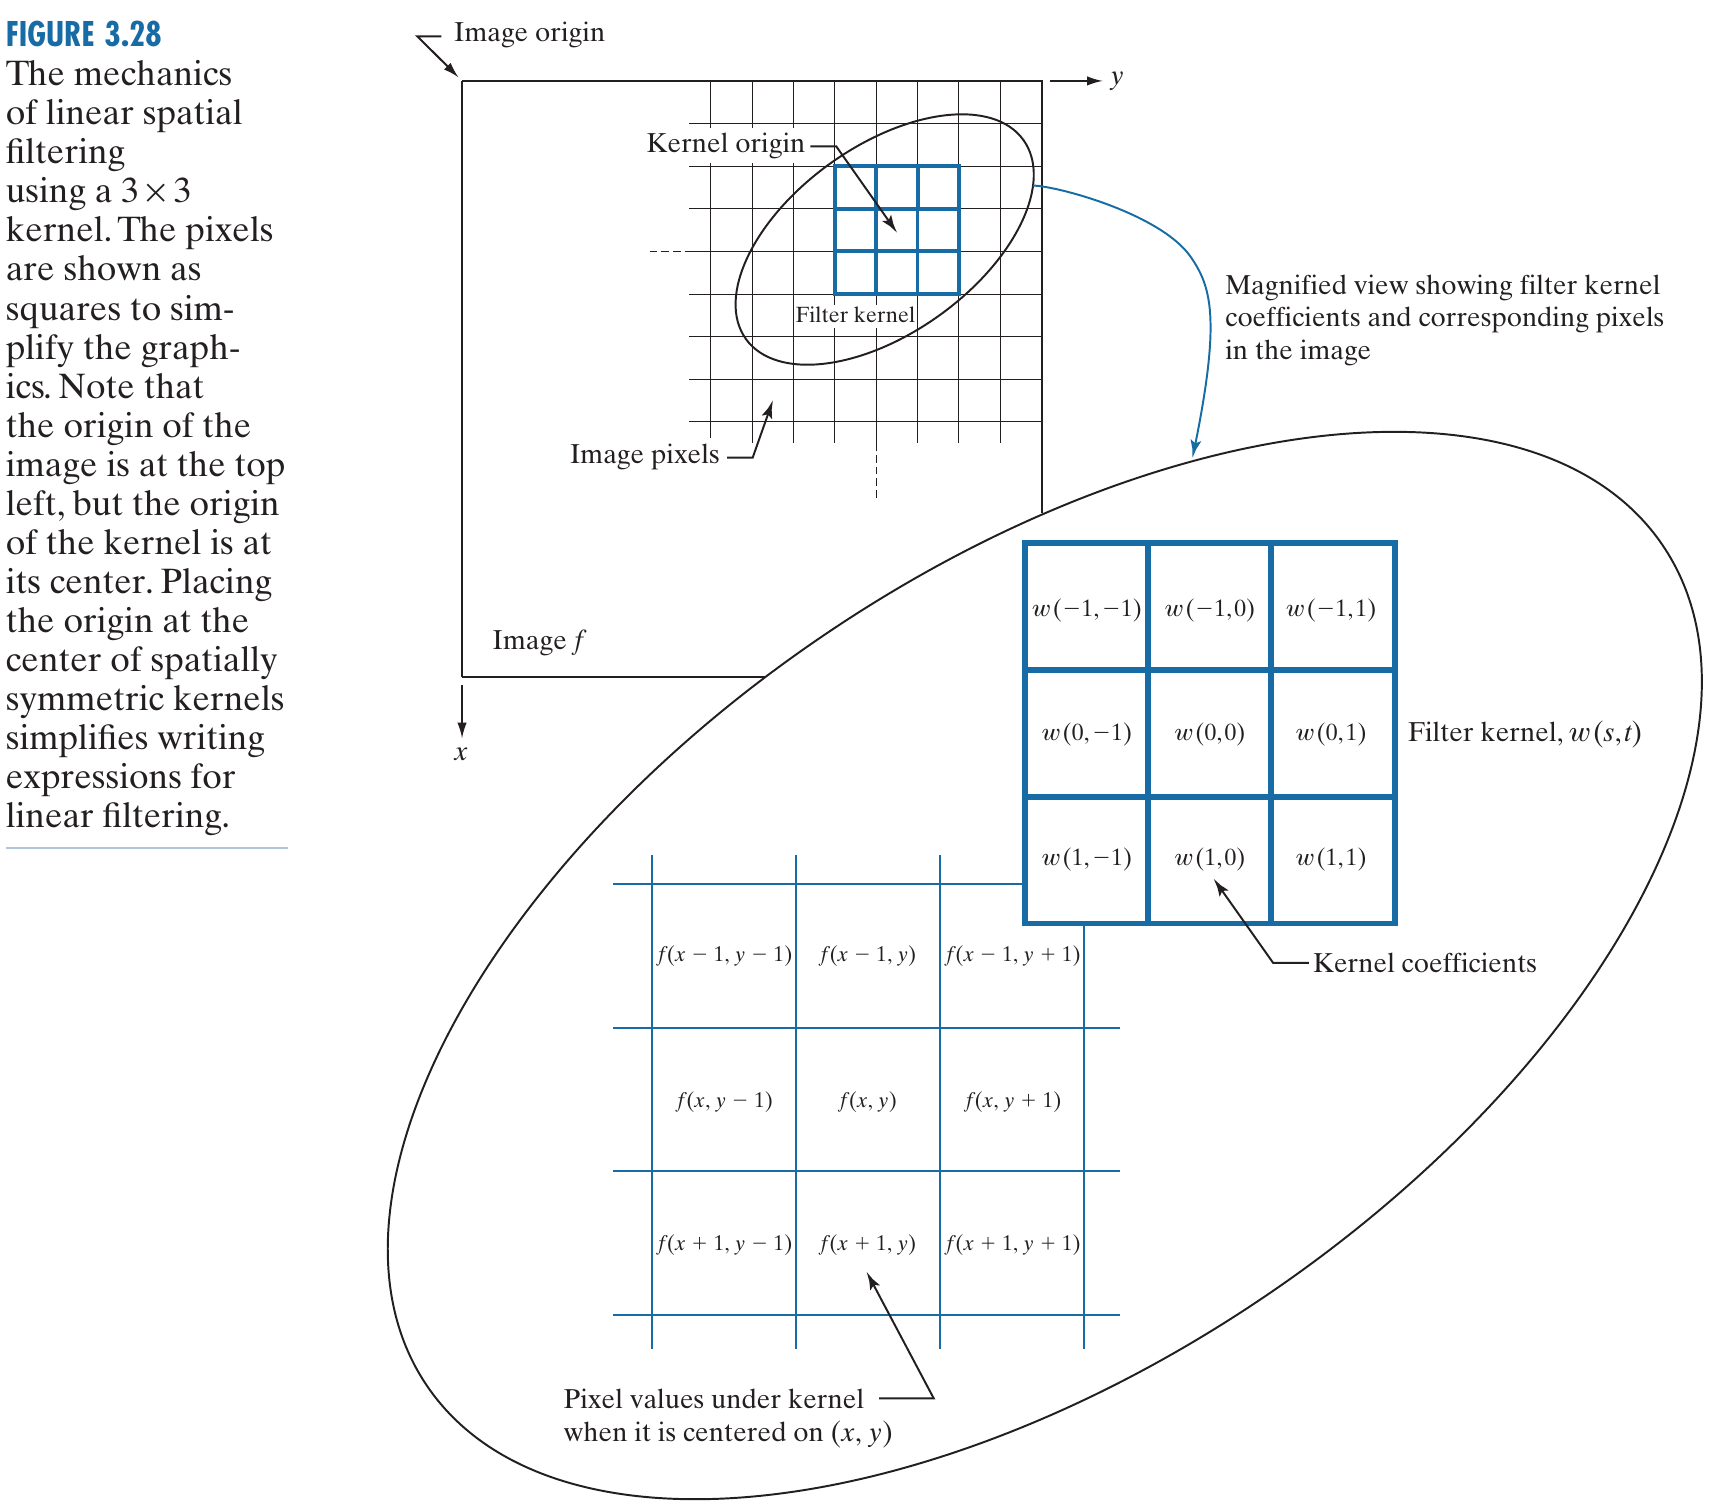
\includegraphics{img/3_3_linear_filtering.png}}
\end{frame}}{\begin{frame}
  \frametitle{相关与卷积}
  
  {\hspace{4em}}\resizebox{0.7\columnwidth}{!}{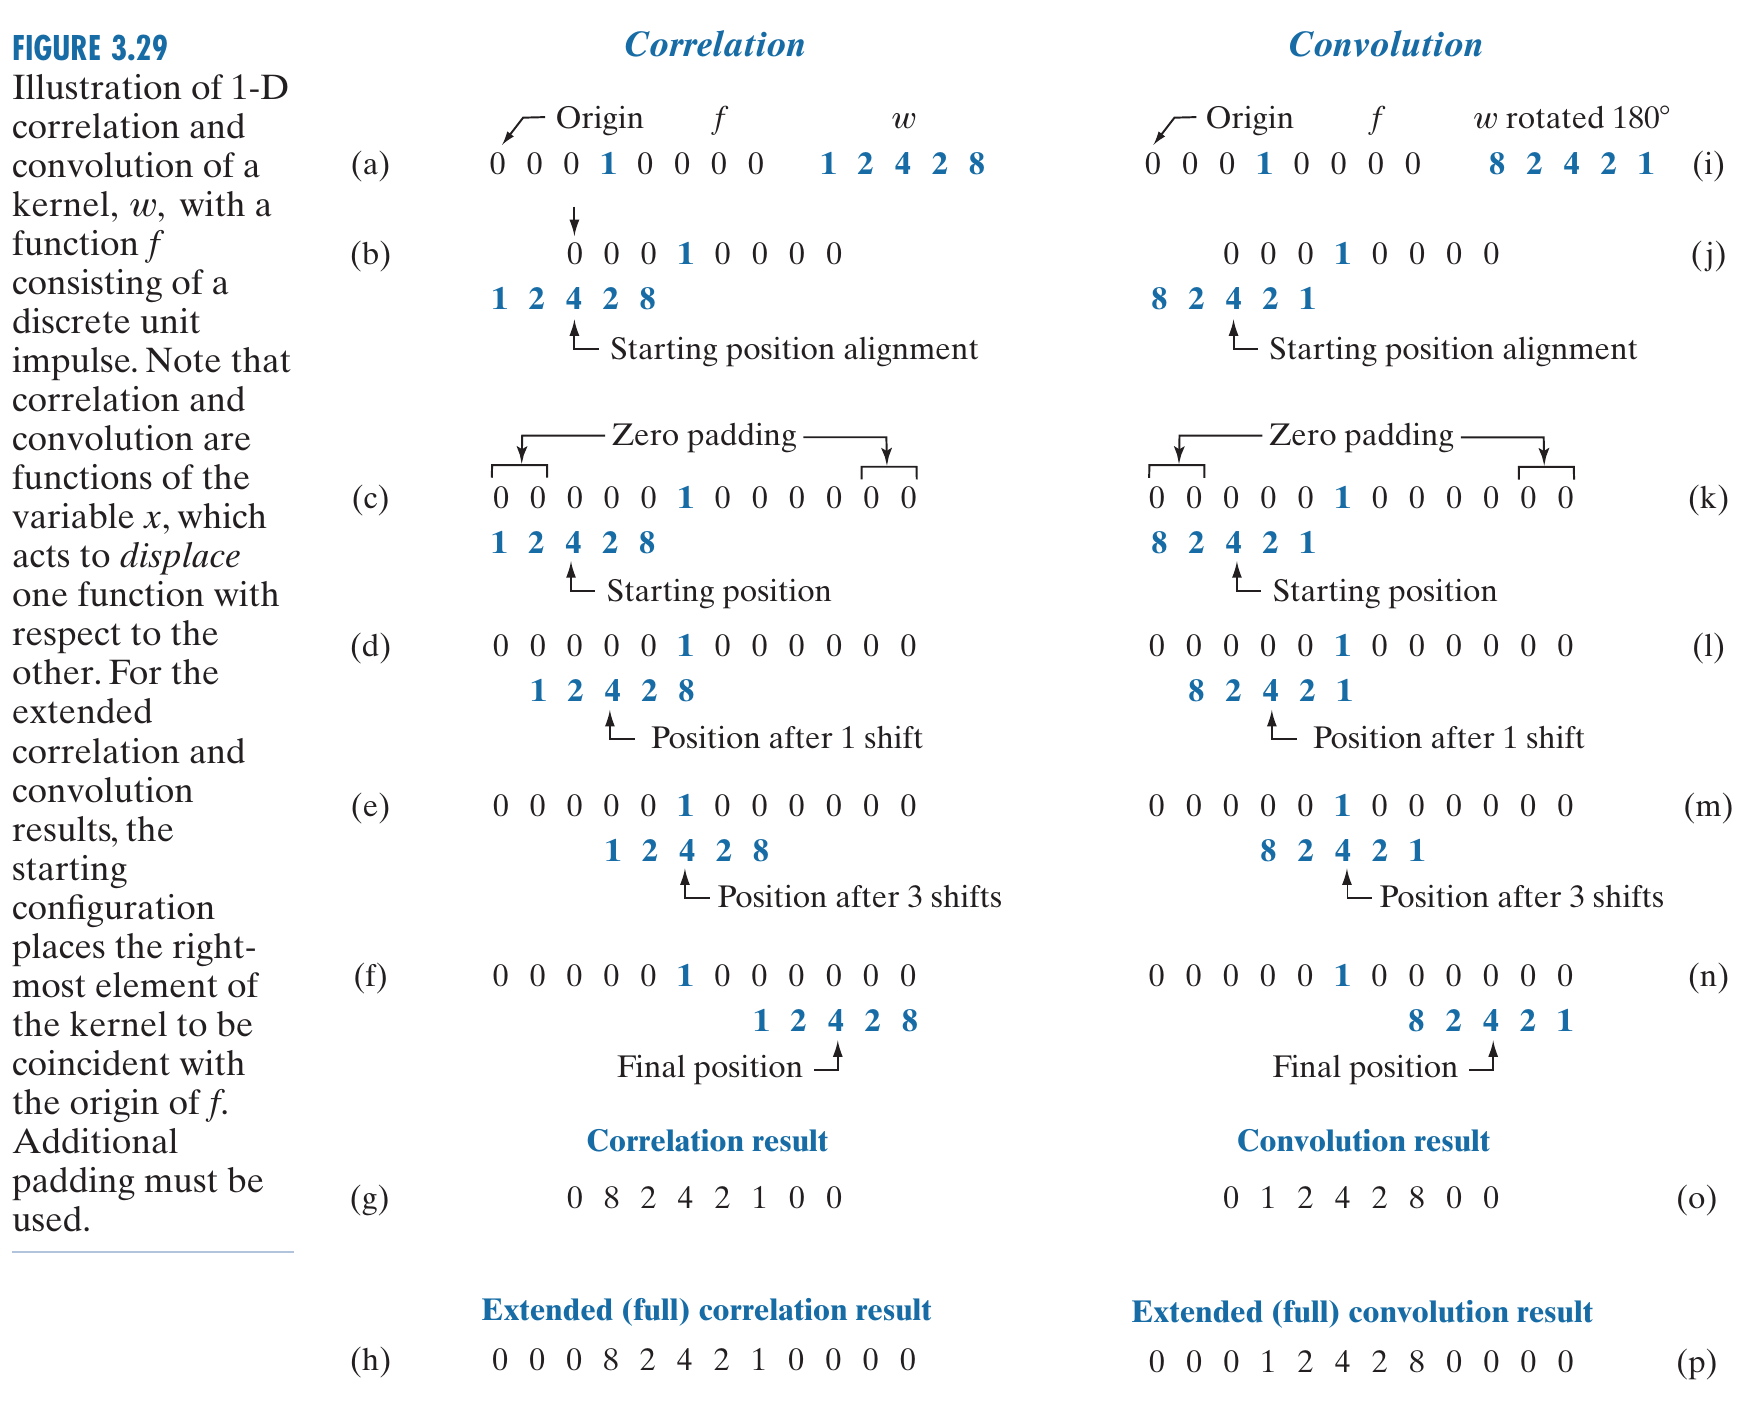
\includegraphics{img/1_D_correlation_convolution.png}}
\end{frame}}{\begin{frame}
  \frametitle{2-D相关与卷积}
  
  \qquad\resizebox{0.8\columnwidth}{!}{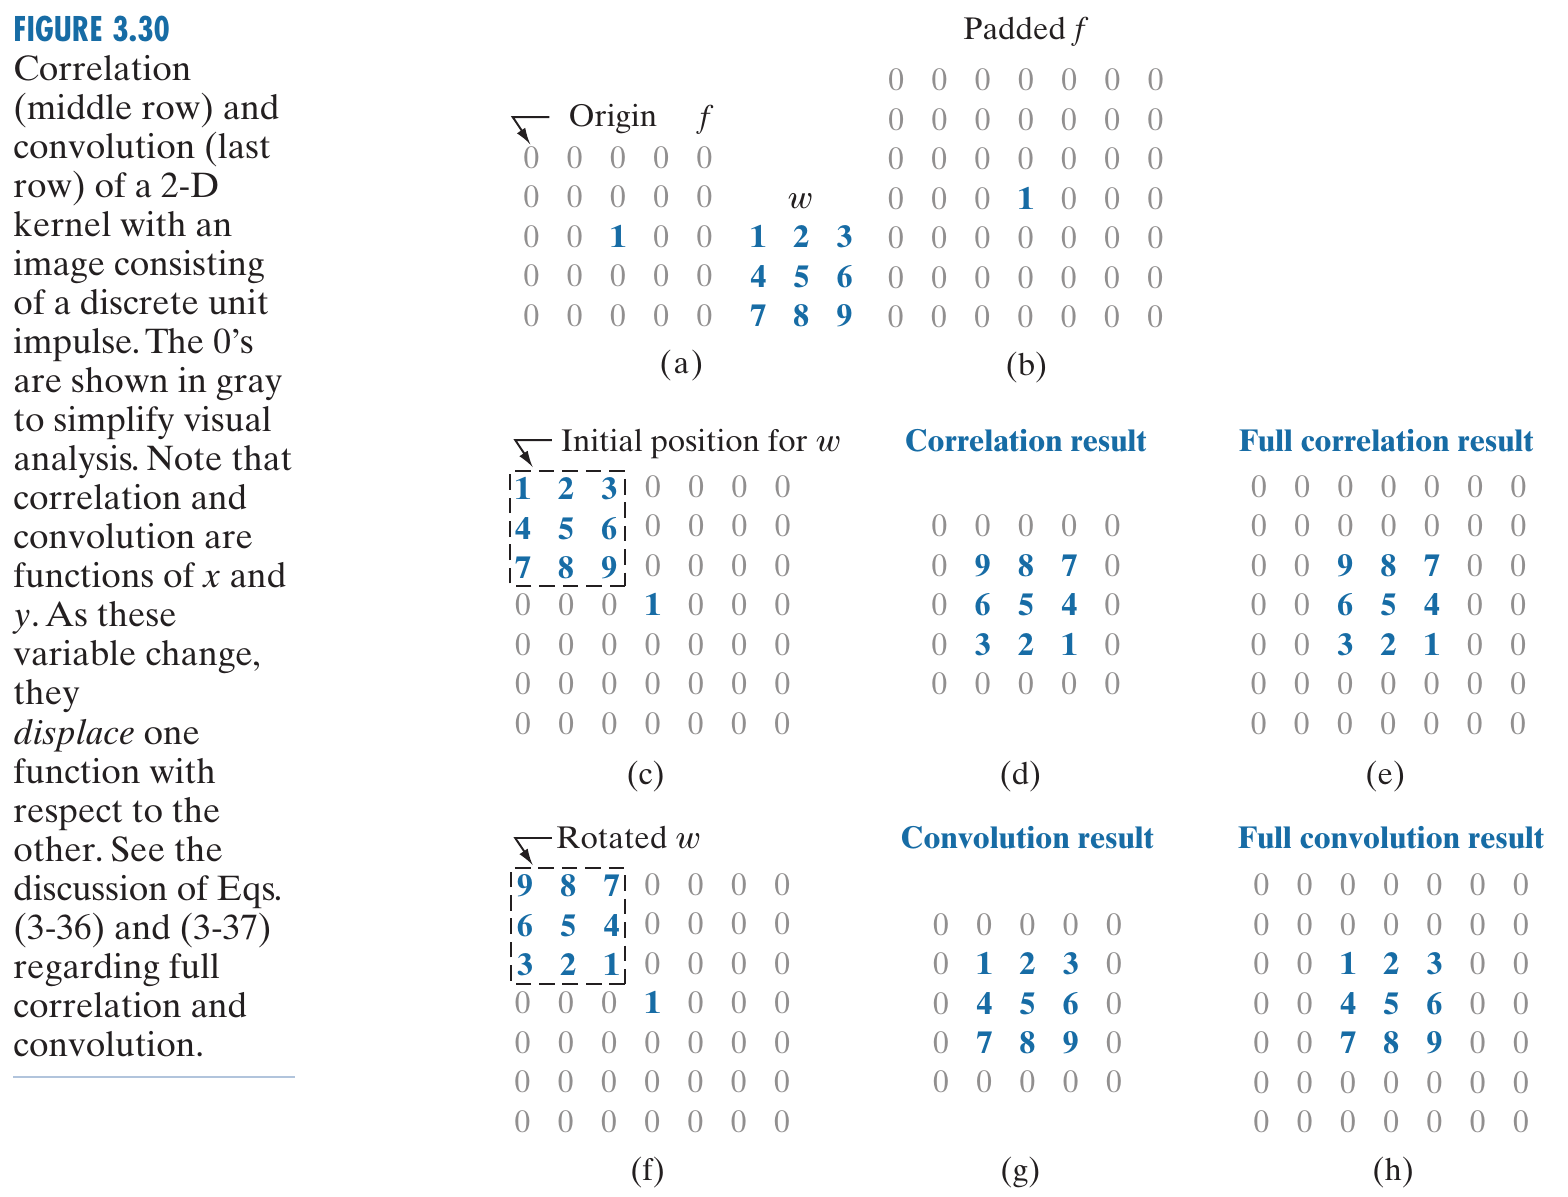
\includegraphics{img/2_D_correlation_convolution.png}}
\end{frame}}{\begin{frame}
  \frametitle{平滑核示例}
  
  \
  
  \
  
  \resizebox{1\columnwidth}{!}{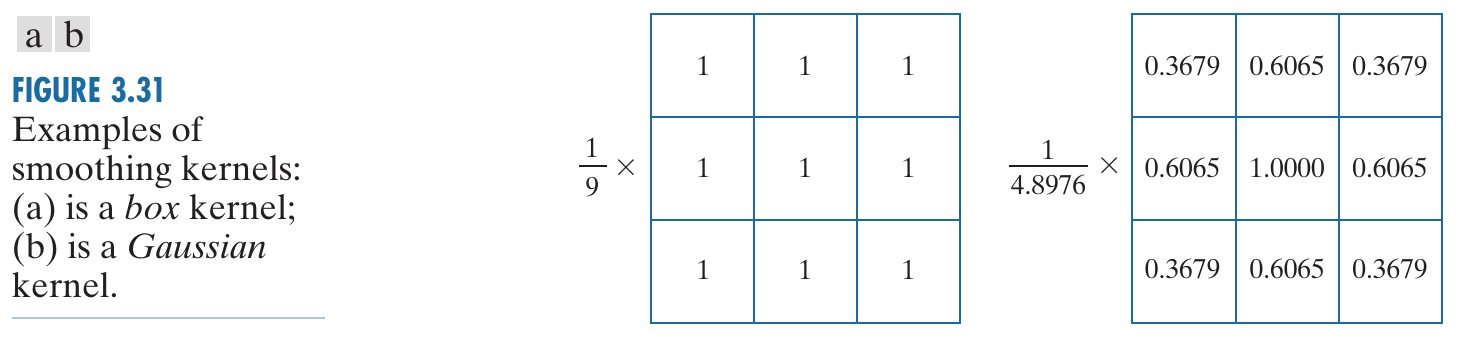
\includegraphics{img/example_smoothing_kernel.png}}
\end{frame}}{\begin{frame}
  \frametitle{空间域与频域低通滤波}
  
  \
  
  \
  
  \resizebox{1\columnwidth}{!}{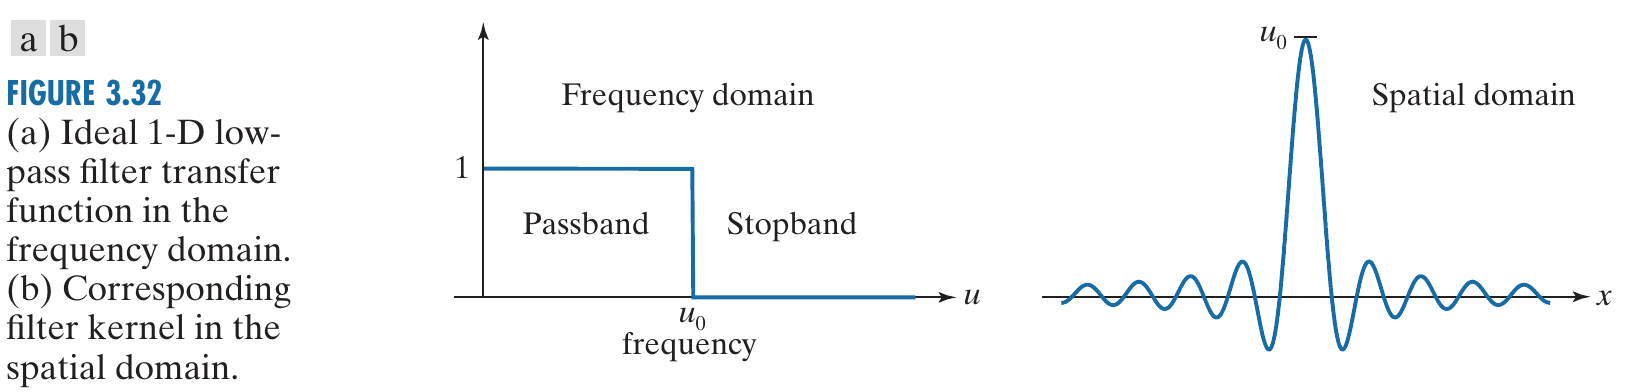
\includegraphics{img/ideal_1_D_low_pass_filter_frequency_domain_spatial_domain.png}}
\end{frame}}{\begin{frame}
  \frametitle{Box kernel}
  
  \quad\resizebox{0.9\columnwidth}{!}{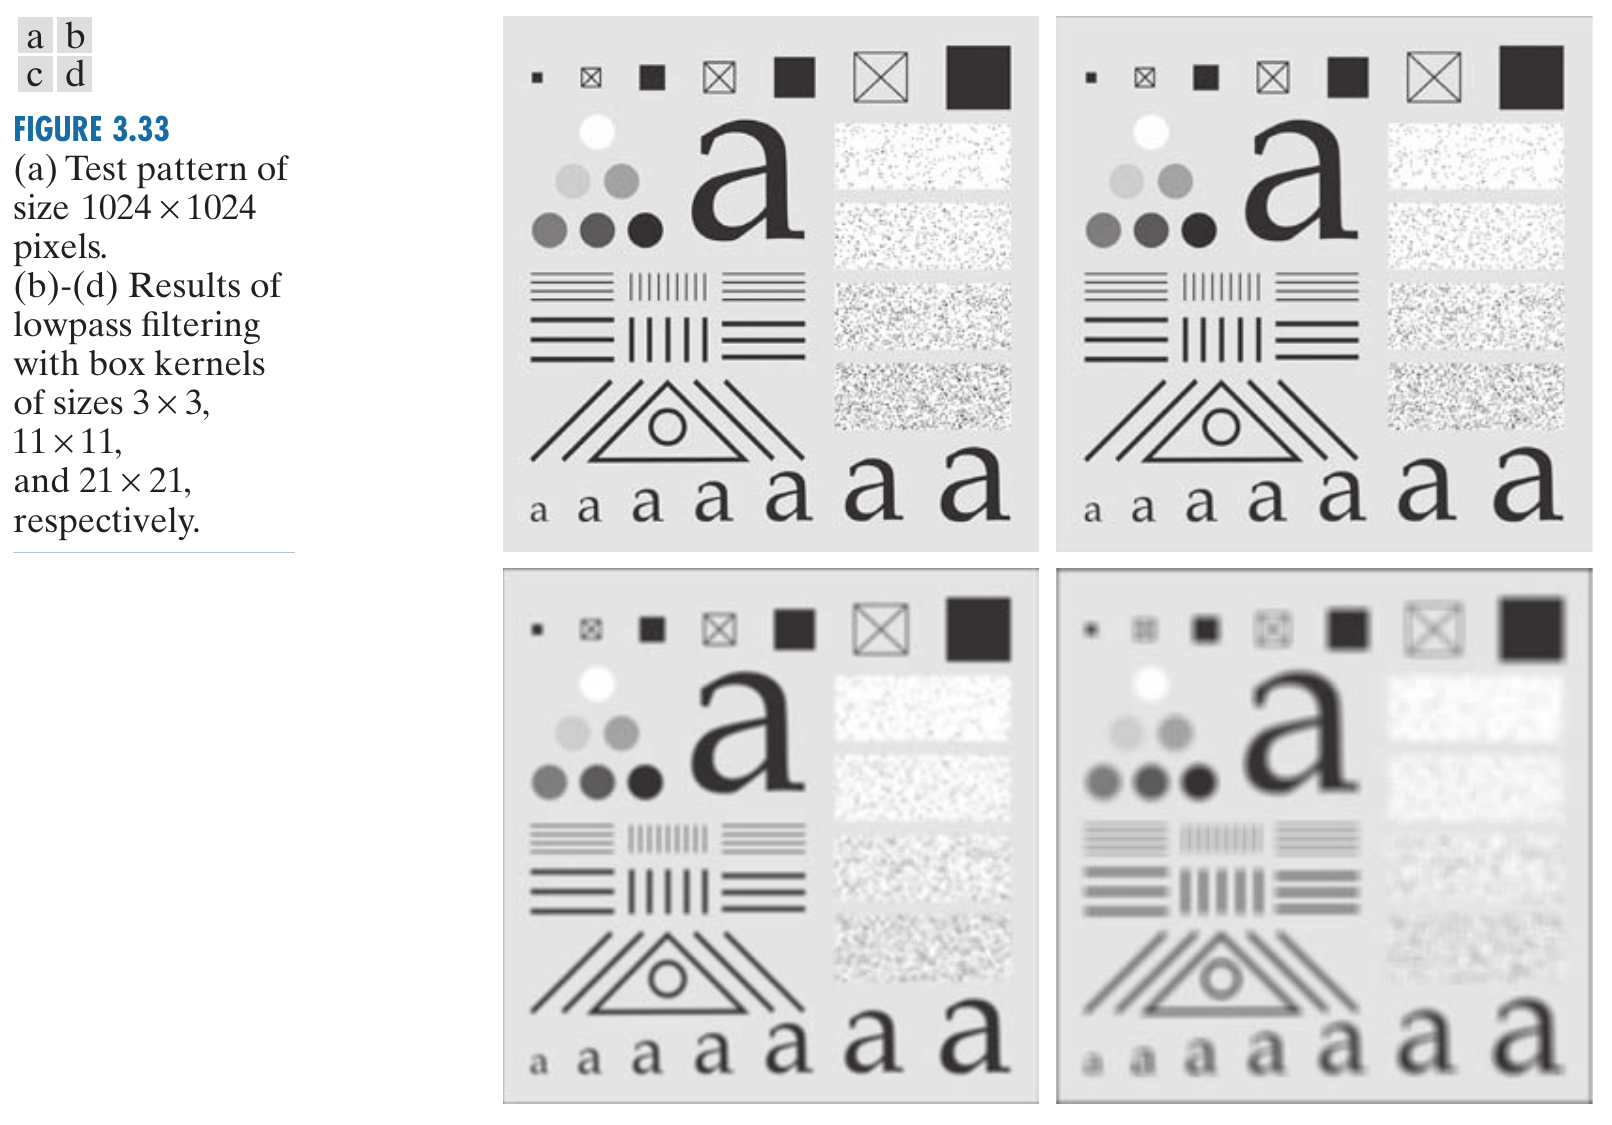
\includegraphics{img/box_filtering.png}}
\end{frame}}{\begin{frame}
  \frametitle{距离}
  
  \resizebox{1\columnwidth}{!}{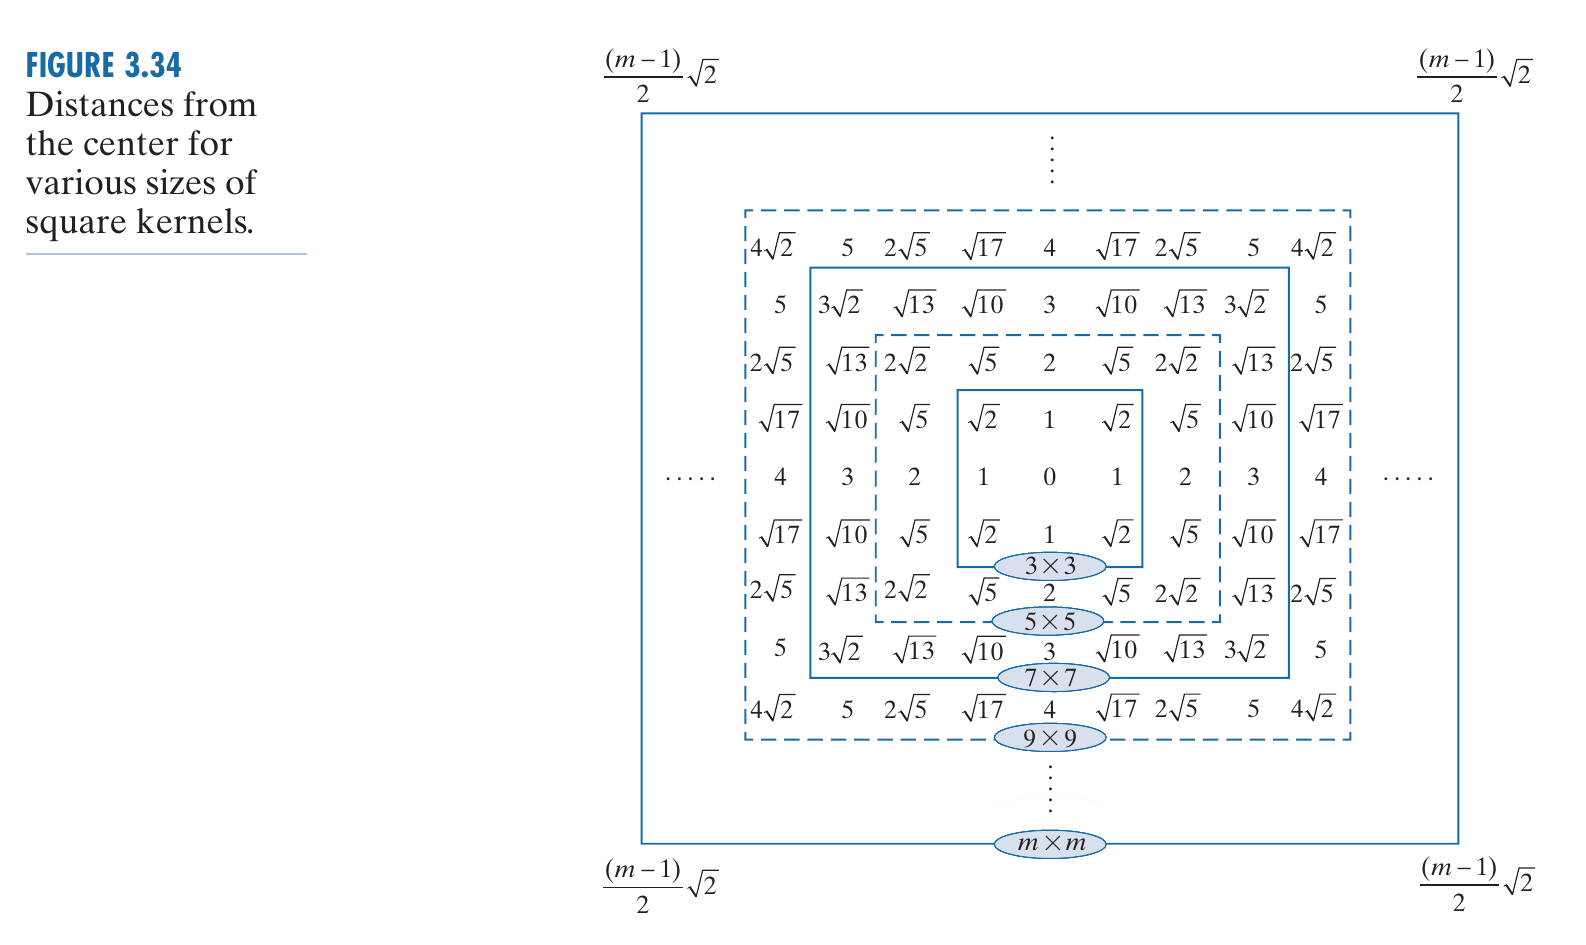
\includegraphics{img/distance.png}}
\end{frame}}{\begin{frame}
  \frametitle{高斯核}
  
  \
  
  \
  
  \resizebox{1\columnwidth}{!}{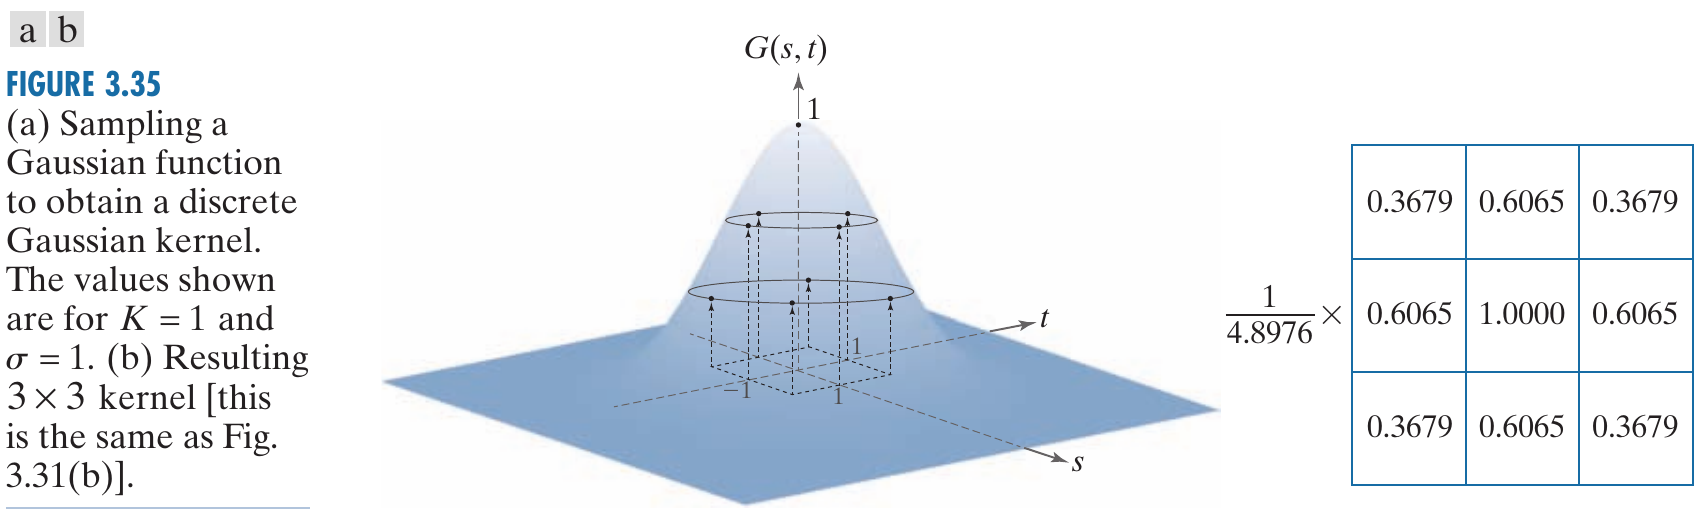
\includegraphics{img/gaussian_kernel.png}}
\end{frame}}{\begin{frame}
  \frametitle{高斯核滤波}
  
  \resizebox{1\columnwidth}{!}{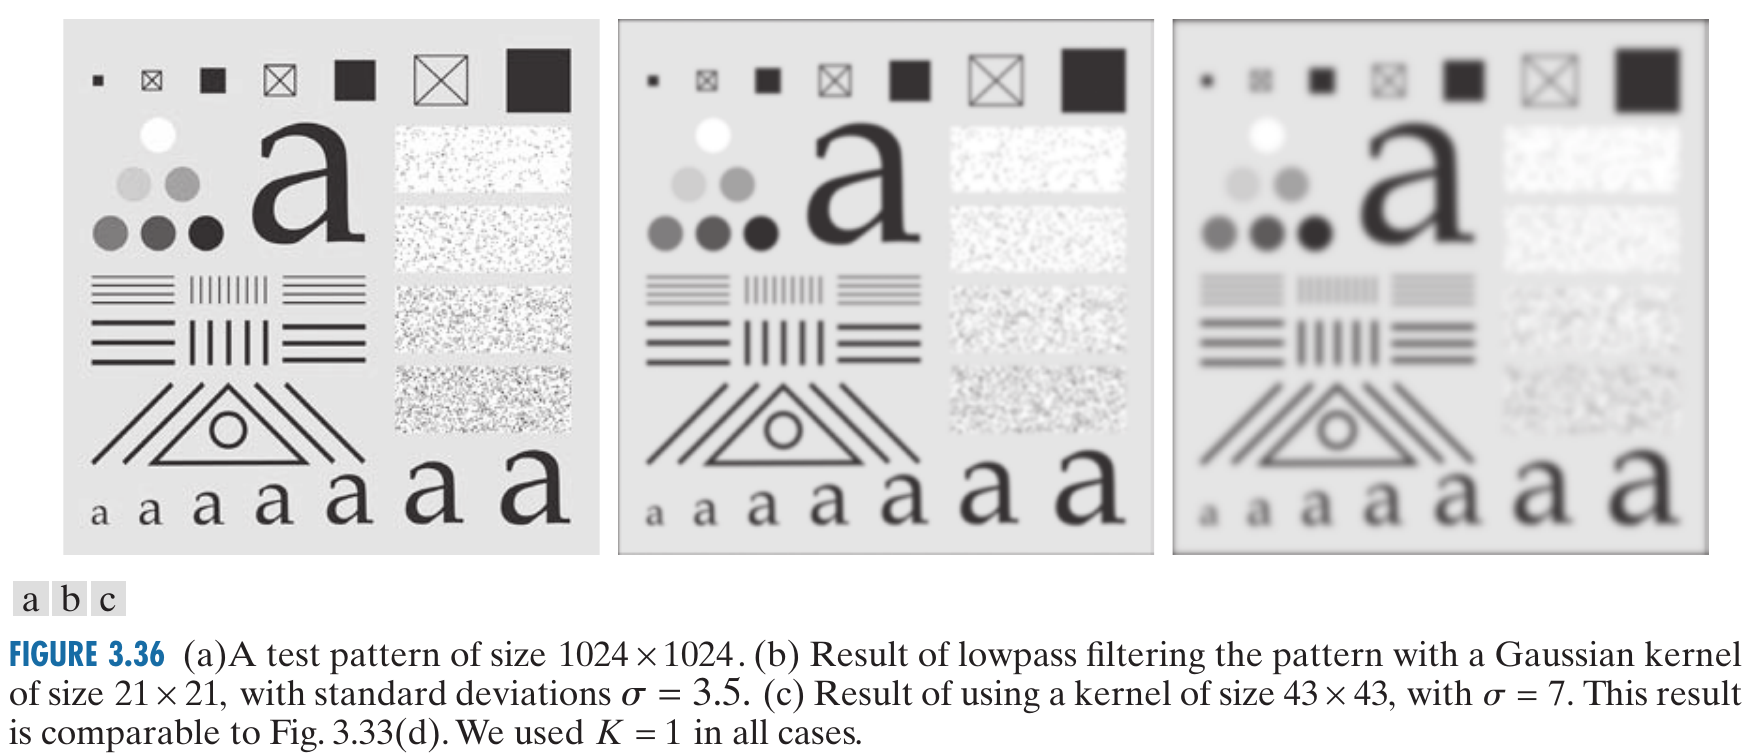
\includegraphics{img/gaussian_kernel_filter.png}}
\end{frame}}{\begin{frame}
  \frametitle{不同尺度高斯滤波}
  
  \
  
  \resizebox{1\columnwidth}{!}{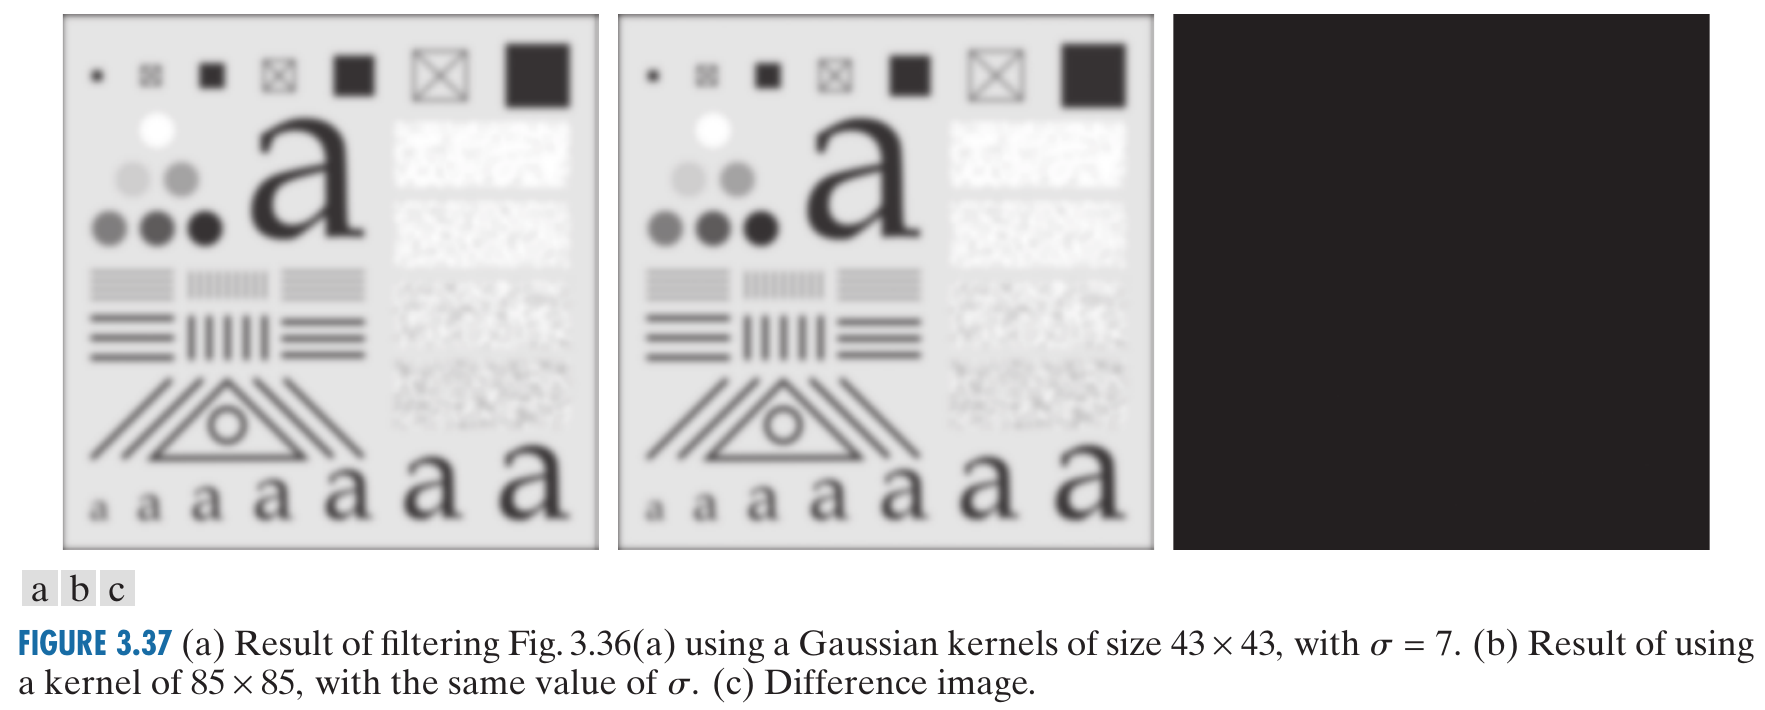
\includegraphics{img/gaussian_kernel_filter_sigma_difference.png}}
  
  \ 
\end{frame}}{\begin{frame}
  \frametitle{平滑效果比较}
  
  \resizebox{1\columnwidth}{!}{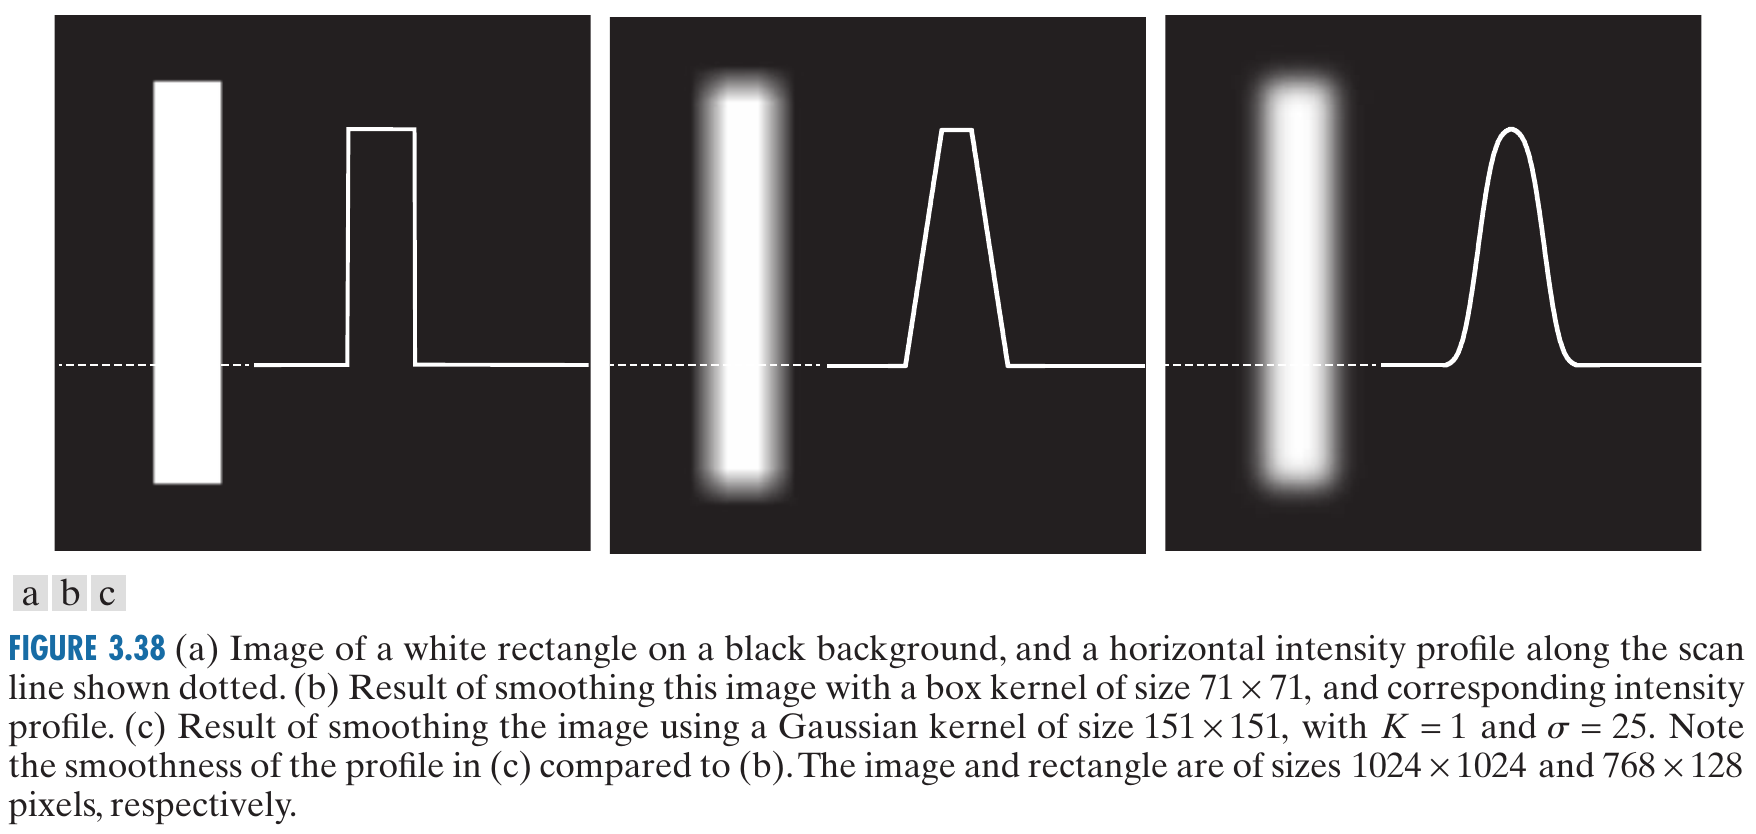
\includegraphics{img/smoothing_box_gaussian_compare.png}}
\end{frame}}{\begin{frame}
  \frametitle{图像大小的影响}
  
  \
  
  \resizebox{1\columnwidth}{!}{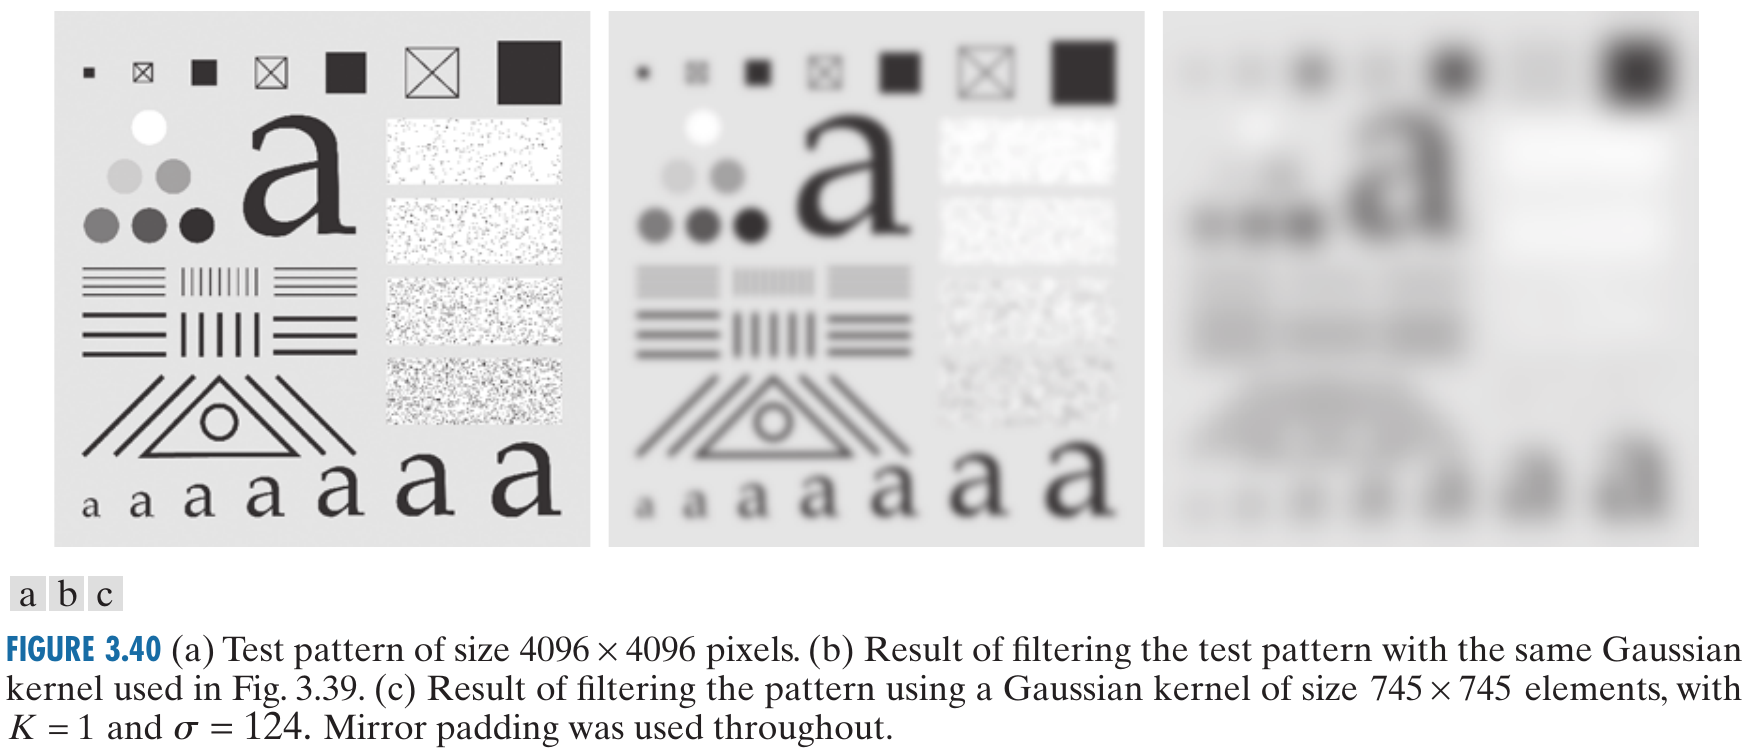
\includegraphics{img/4096_gaussian_kernel.png}}
\end{frame}}{\begin{frame}
  \frametitle{低通阈值区域提取}
  
  \
  
  \
  
  \resizebox{1\columnwidth}{!}{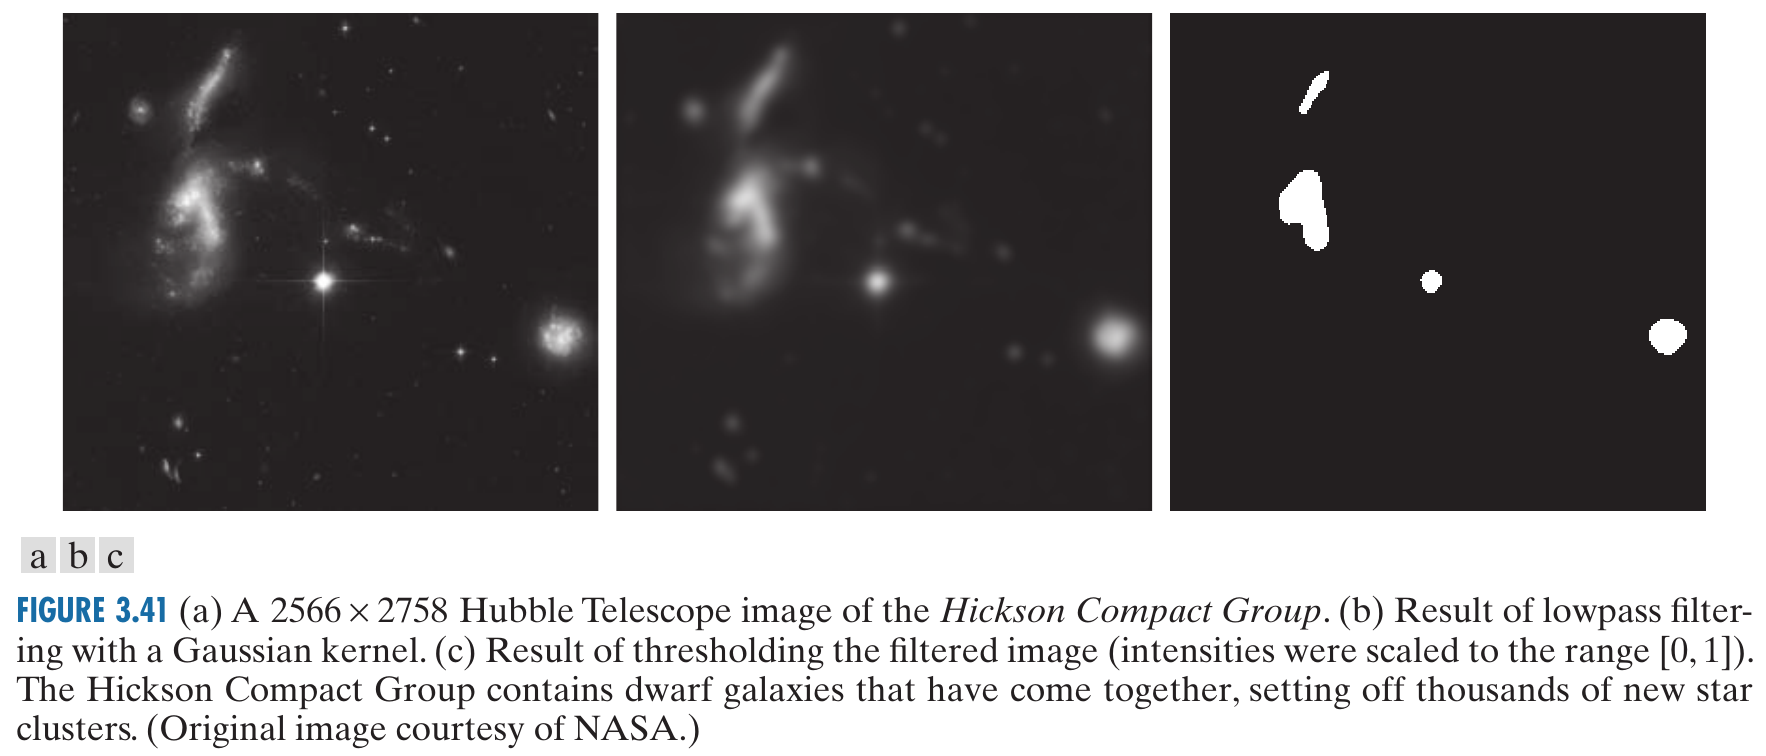
\includegraphics{img/lowpass_threshold_region_extraction.png}}
\end{frame}}{\begin{frame}
  \frametitle{渐晕校正}
  
  \
  
  \resizebox{1\columnwidth}{!}{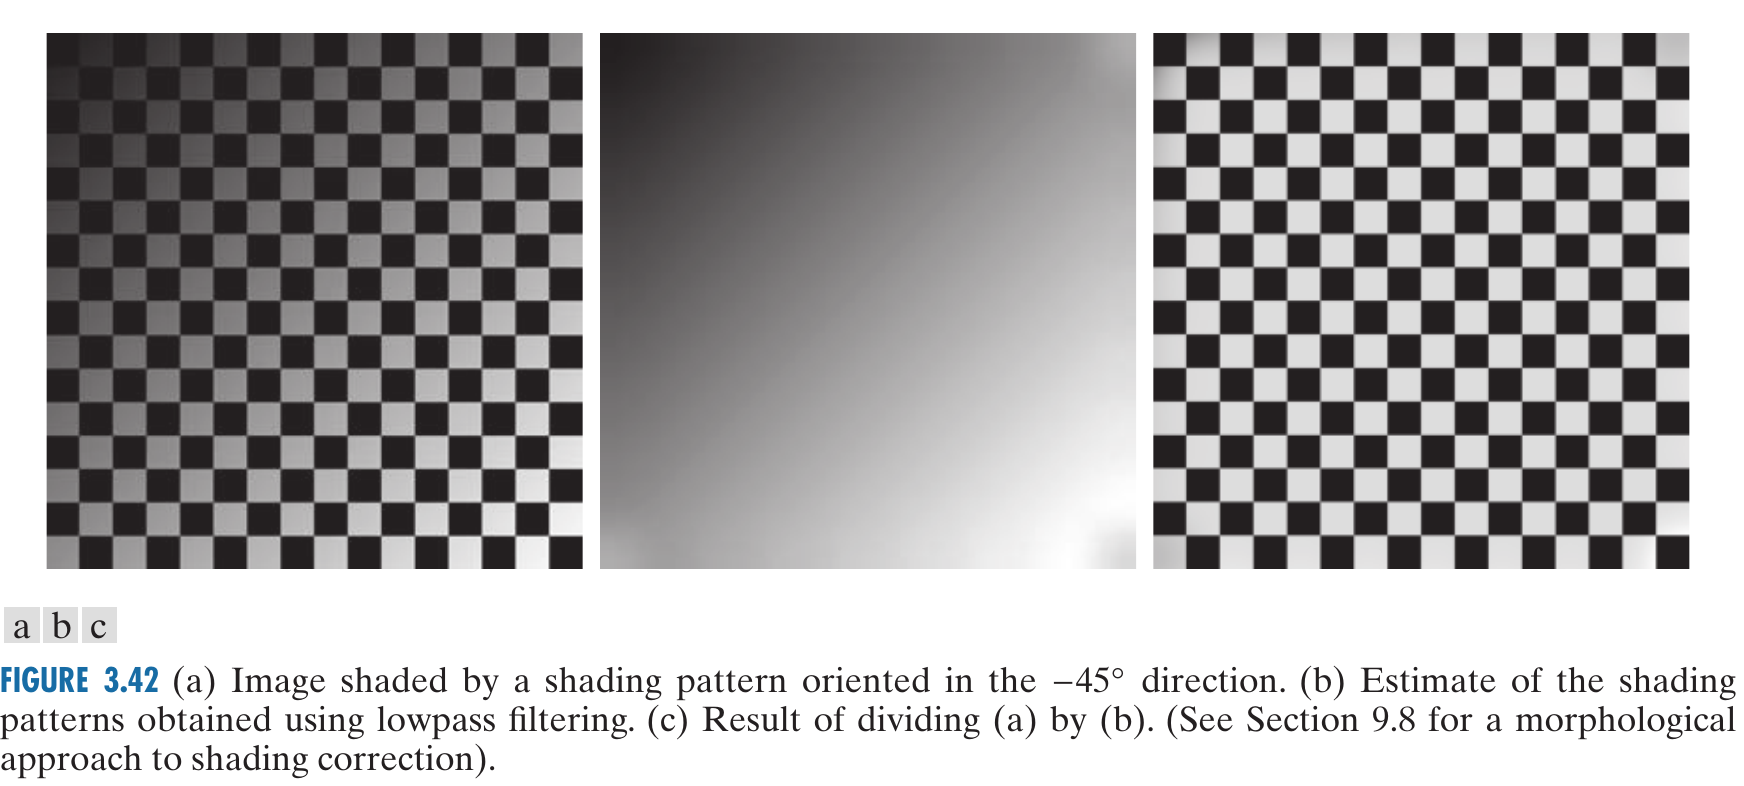
\includegraphics{img/shading_correction.png}}
\end{frame}}{\begin{frame}
  \frametitle{次序统计滤波}
  
  \
  
  \
  
  \resizebox{1\columnwidth}{!}{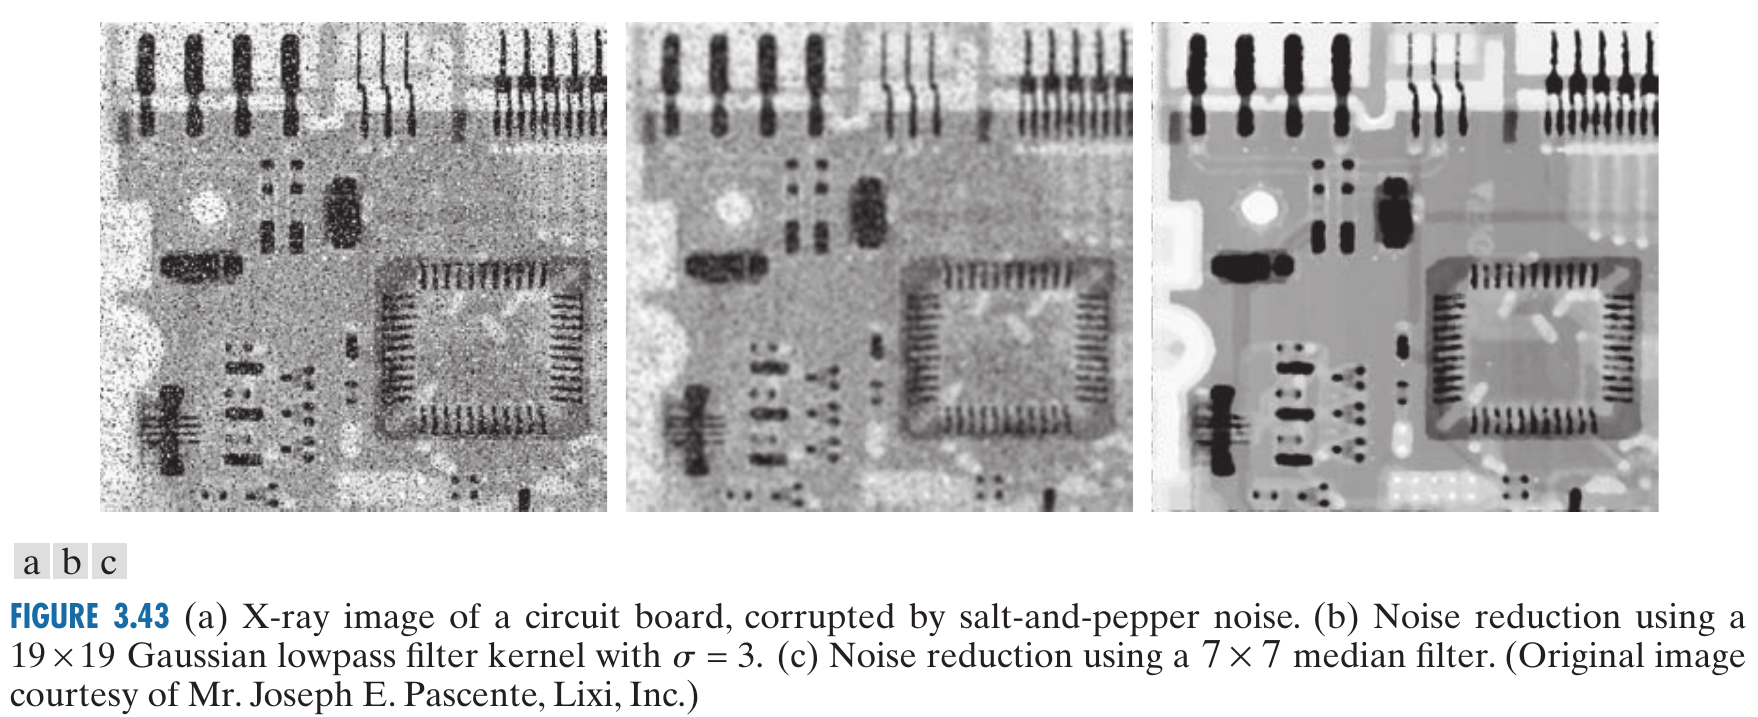
\includegraphics{img/x_ray_image_mean_median.png}}
\end{frame}}{\begin{frame}
  \frametitle{一阶与二阶导数}
  
  \quad\resizebox{0.9\columnwidth}{!}{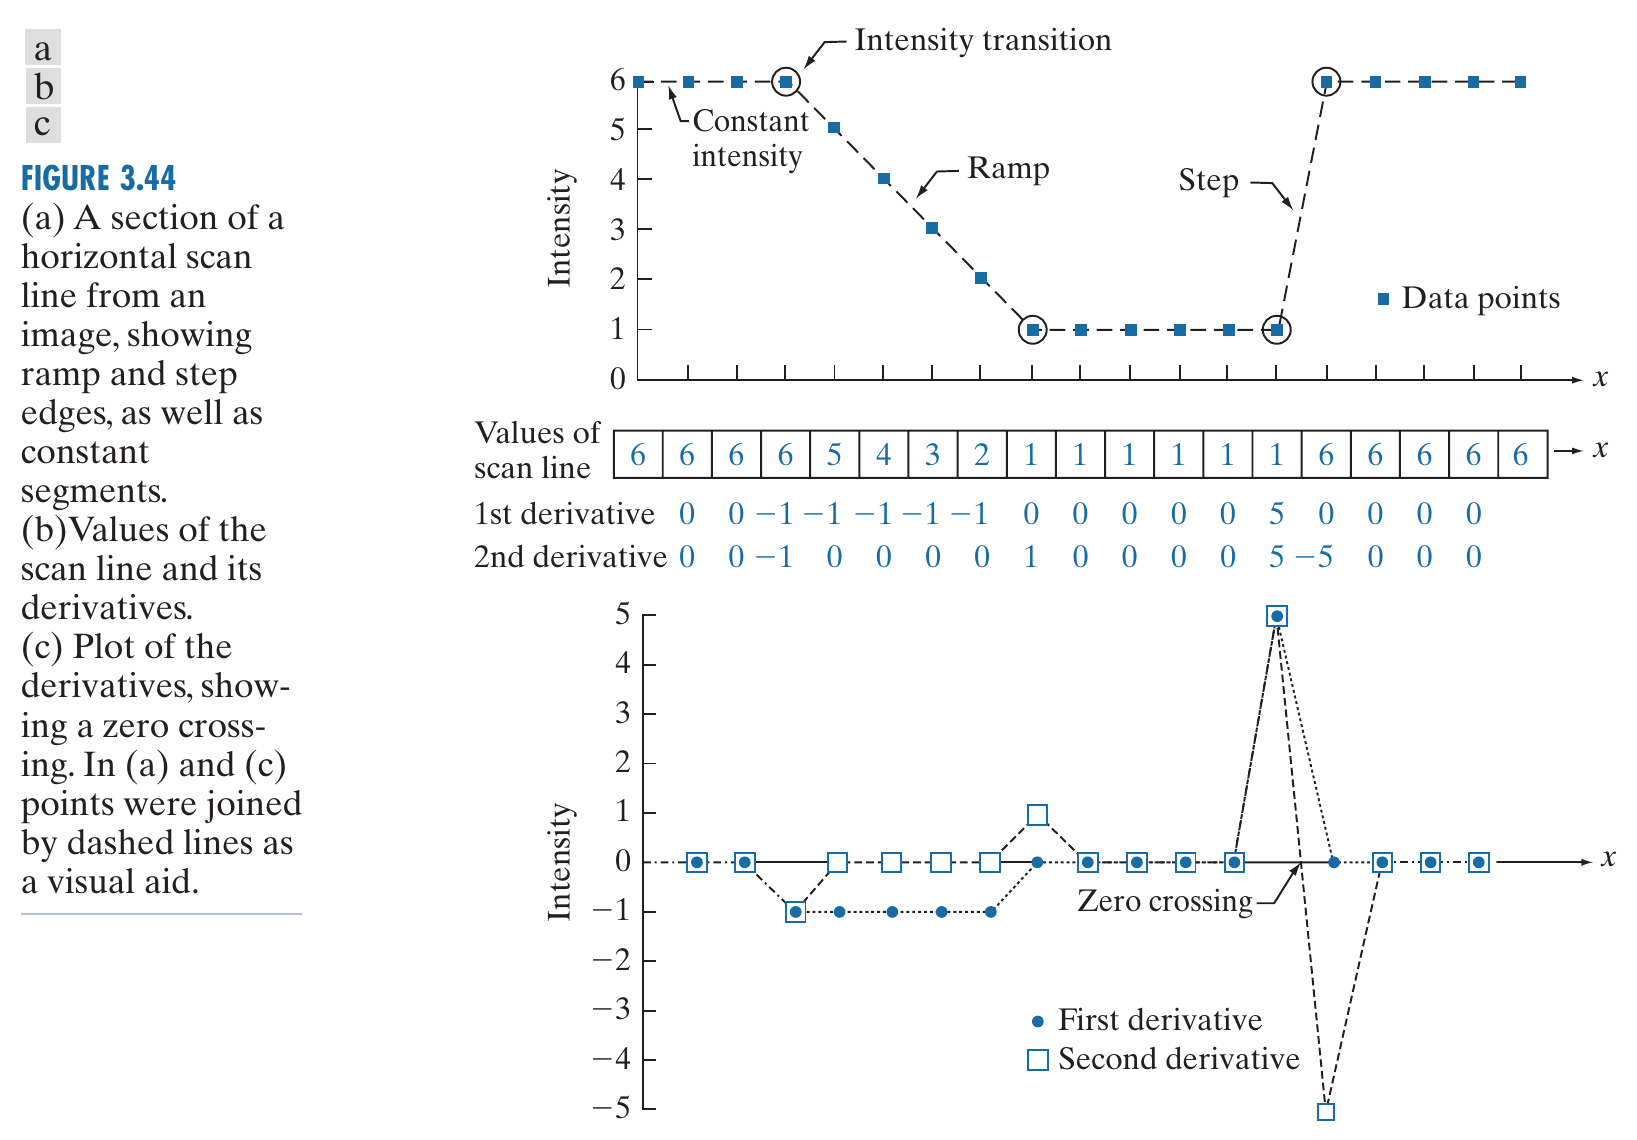
\includegraphics{img/1_2_derivative.png}}
\end{frame}}{\begin{frame}
  \frametitle{Laplacian kernel}
  
  \
  
  \resizebox{1\columnwidth}{!}{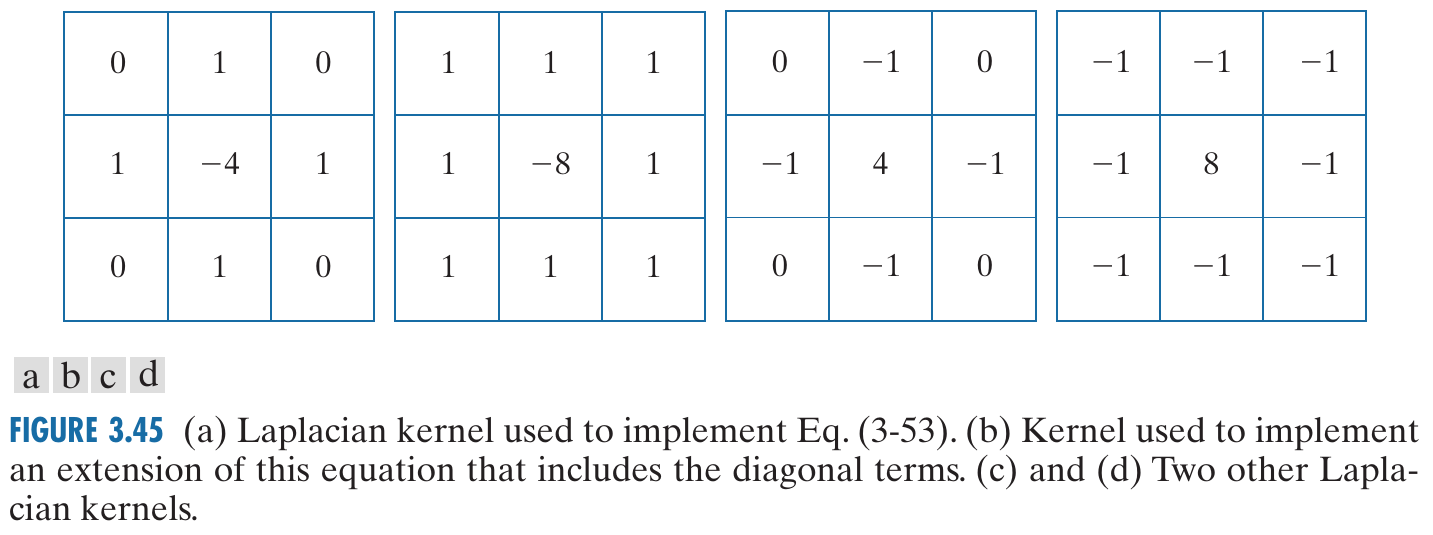
\includegraphics{img/laplacian_kernel.png}}
\end{frame}}{\begin{frame}
  \frametitle{图像锐化示例}
  
  {\hspace{4em}}\resizebox{0.7\columnwidth}{!}{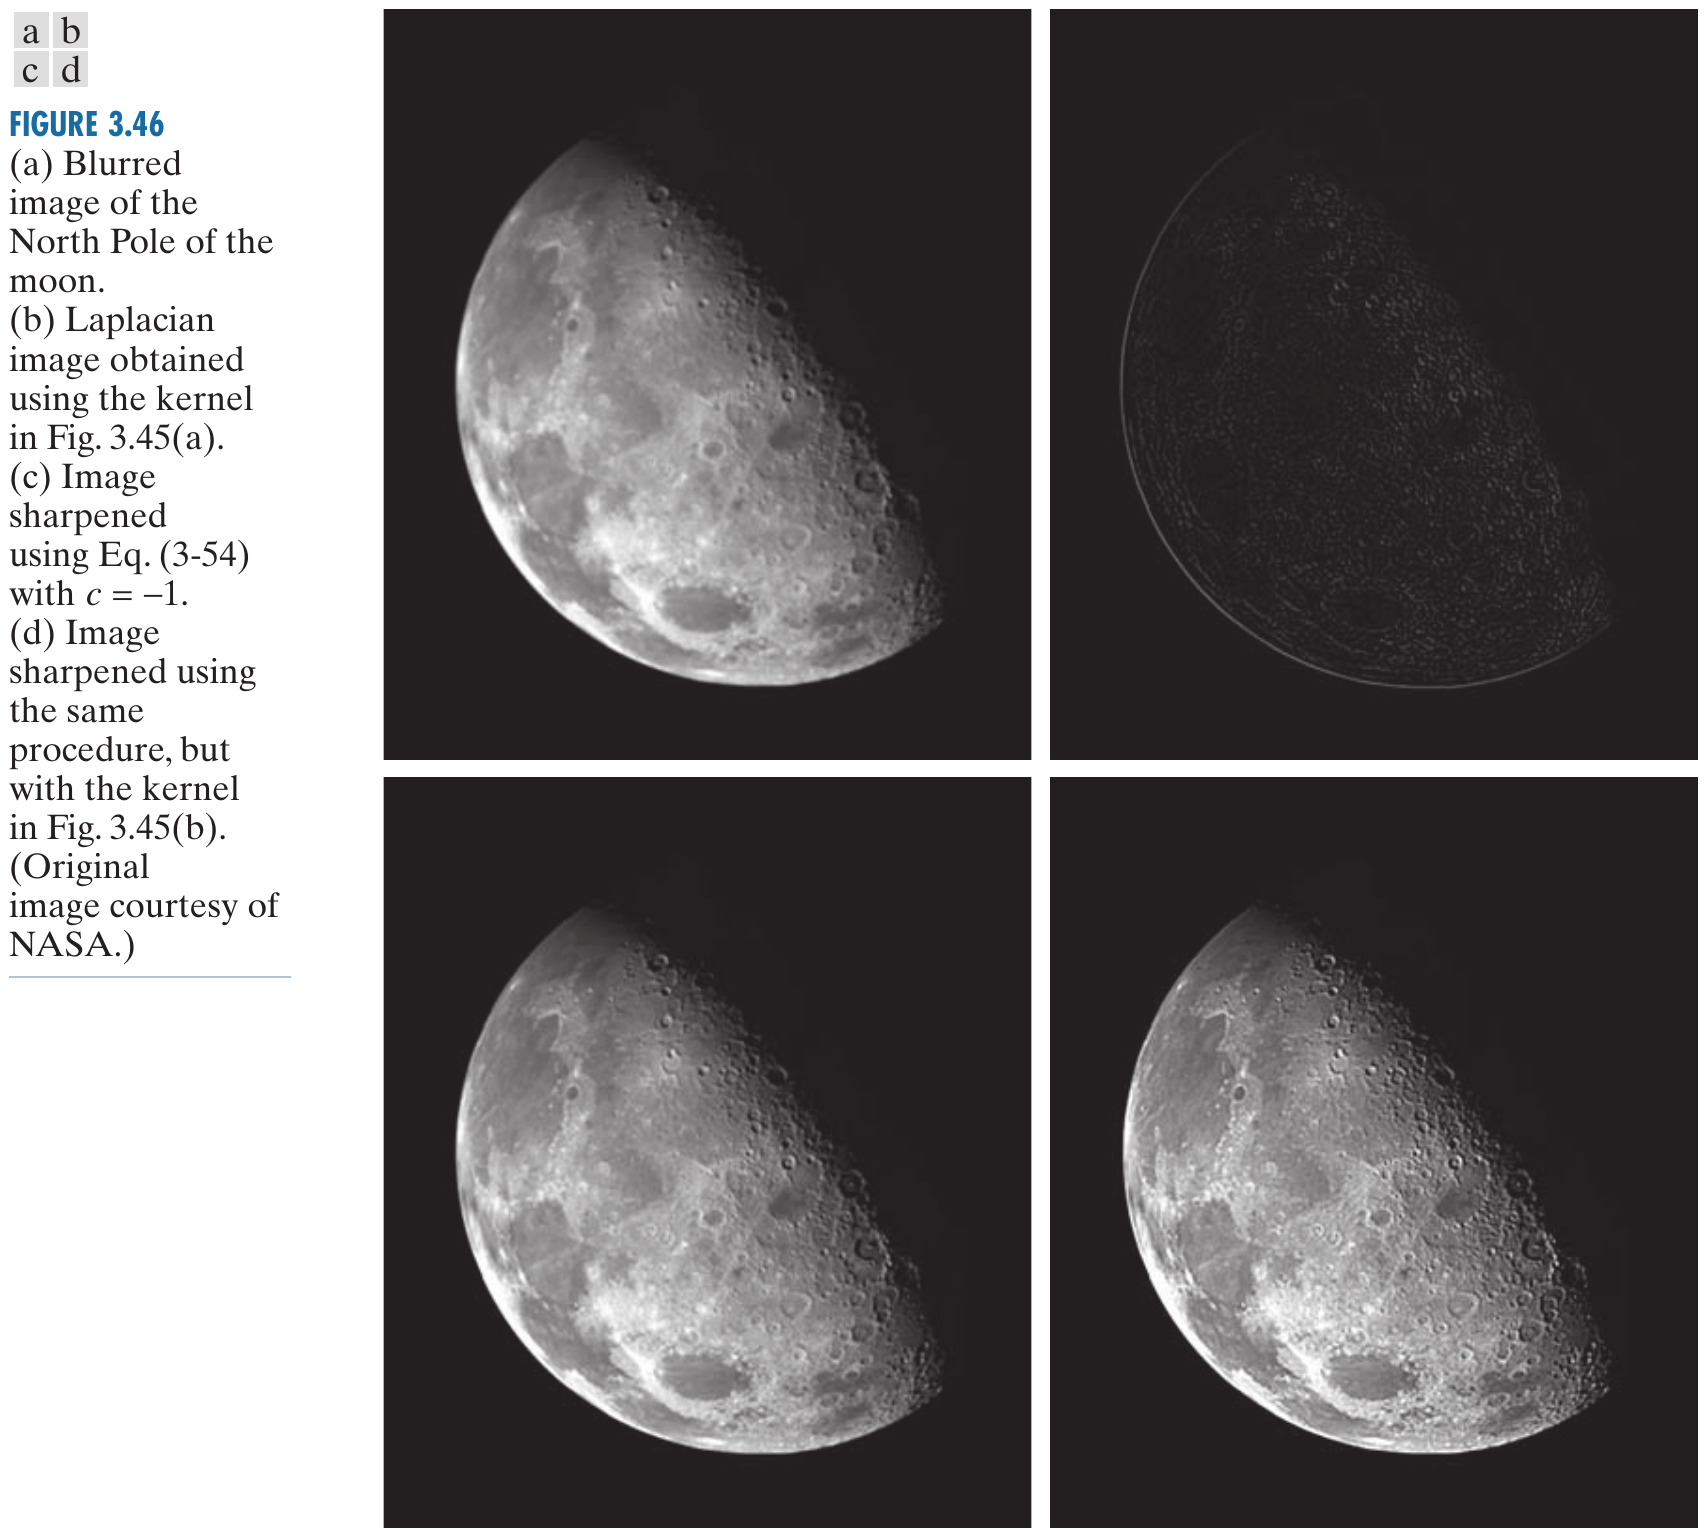
\includegraphics{img/sharpening_laplacian.png}}
\end{frame}}{\begin{frame}
  \frametitle{图像锐化示例(续)}
  
  \resizebox{1\columnwidth}{!}{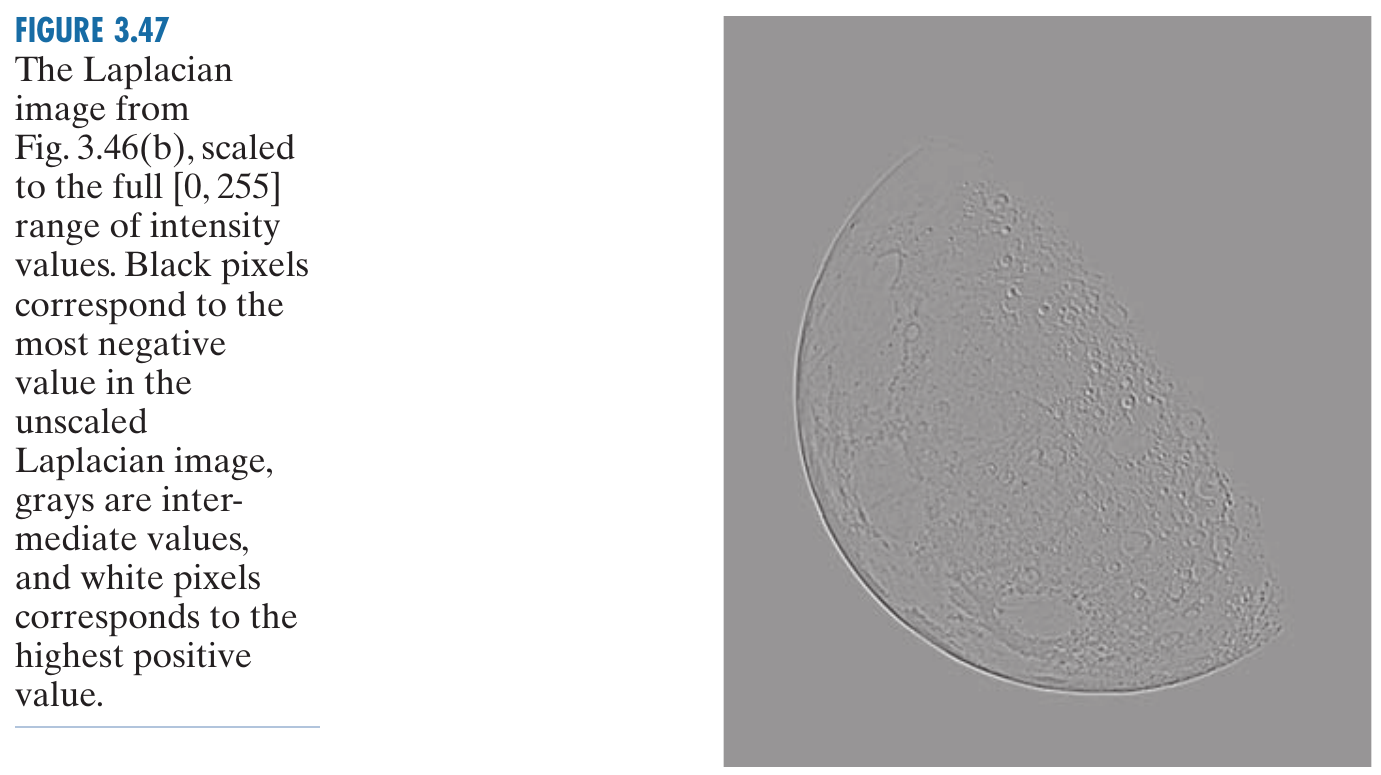
\includegraphics{img/sharping_laplacian_image.png}}
\end{frame}}{\begin{frame}
  \frametitle{反锐化掩模}
  
  \quad\resizebox{0.9\columnwidth}{!}{\includegraphics{img/unsharp_mask.png}}
\end{frame}}{\begin{frame}
  \frametitle{锐化示例}
  
  \
  
  \resizebox{1\columnwidth}{!}{\includegraphics{img/unsharp_masking_highboost_filtering.png}}
\end{frame}}{\begin{frame}
  \frametitle{梯度}
  
  \quad\resizebox{0.9\columnwidth}{!}{\includegraphics{img/roberts_sobel.png}}
\end{frame}}{\begin{frame}
  \frametitle{边缘增强}
  
  \
  
  \resizebox{1\columnwidth}{!}{\includegraphics{img/sobel_gradient.png}}
\end{frame}}{\begin{frame}
  \frametitle{高通、带通滤波器}
  
  \
  
  \resizebox{1\columnwidth}{!}{\includegraphics{img/lowpass_highpass_bandreject_bandpass.png}}
\end{frame}}{\begin{frame}
  \frametitle{示例图像}
  
  \resizebox{1\columnwidth}{!}{\includegraphics{img/zone_plate_image.png}}
\end{frame}}{\begin{frame}
  \frametitle{1维与2维滤波器}
  
  \
  
  \resizebox{1\columnwidth}{!}{\includegraphics{img/1D_2D_gaussian_filter.png}}
\end{frame}}{\begin{frame}
  \frametitle{不同滤波效果}
  
  \
  
  \resizebox{1\columnwidth}{!}{\includegraphics{img/separable_isotropic_filter.png}}
\end{frame}}{\begin{frame}
  \quad\resizebox{0.9\columnwidth}{!}{\includegraphics{img/zone_plate_lowpass_highpass_band.png}}
\end{frame}}{\begin{frame}
  \frametitle{空间域图像增强}
  
  {\hspace{6em}}\resizebox{0.5\columnwidth}{!}{\includegraphics{img/spatial_enhancement1.png}}
\end{frame}}{\begin{frame}
  \frametitle{空间域图像增强}
  
  {\hspace{6em}}\resizebox{0.5\columnwidth}{!}{\includegraphics{img/spatial_enhancement2.png}}
\end{frame}}}

\end{document}
